\subsection{Statistical Methods}
We derive upper limits on the product of the Higgs boson production
cross section and the $\Hi \to \WW$ branching fraction,
$\sigma_{\rm{H}} \times $BR($\Hi \to \WW)$, with respect to the SM
expectation, i.e. $\sigma^{95\%}/\sigma^{SM}$. Two different
statistical methods are used to report results. The first method is
based on Bayesian inference~\cite{bayesian} and the second one, known
as $CL_{s}$, is the modified frequentist approach~\cite{cls1,cls2}.

The likelihood function is defined as:
\begin{eqnarray}
  L(\rm{data}|\mu,\theta)&=&\rm{Poisson}(\rm{data}|\mu\cdot s(\theta)+b(\theta))\cdot p(\tilde{\theta}|\theta) \nonumber\\
 &=&\prod_i\frac{(\mu s_i+b_i)^{n_i}}{n_i!}e^{-\mu s_i-b_i}\cdot p(\tilde{\theta}|\theta)
\label{eq:likelihood}
\end{eqnarray}
where $\mu$ is the signal strength modifier which is often reported in
the upper limit results as a ratio of the cross-section upper limit
over the standard model cross-section and $\theta$ represents a full
set of nuisance parameters that are used to incorporate systematic
uncertainties. 

The first method (Bayesian) is based on interpreting the likelihood
(Eq.~\ref{eq:likelihood}) as a probability distribution function with
a flat prior for the signal strength and a set of pdfs for nuisance
parameters, which are often approximated with the log-normal
distribution. Integrating over the nuisance parameters we find the
upper limit for the signal strength.

For $CL_{s}$ method the test statistic is defined as a likelihood
ratio:
\begin{equation}
\tilde{q_\mu}=-2\log\frac{L(\rm{data}|\mu,\hat\theta_\mu)}{L(\rm{data}|\hat\mu,\hat\theta)}
\end{equation}
where the numerator corresponds to the maximum likelihood for given
``data'' and $\mu$ profiling over the nuisance parameters and the
denominator corresponds to the maximum likelihood for given ``data''
profiling over the nuisance parameters and $\mu$. This test statistic
differs from the ones used at LEP (no profiling of systematic errors)
and at Tevatron (the denominator likelihood uses $\mu=0$ and only
systematic errors are profiled).

The results obtained using the two methods may differ but in most cases
they are very close. To perform the computation of the limits, the
software packages
\texttt{RooStats}~\cite{rootstat} and \texttt{LandS}~\cite{lands} have 
been used.

\subsection{Background Estimation}

The estimation of the backgrounds follows the strategies described in
Section~\ref{sec:backgrounds}. 

First we estimate the $\dyll$ at the WW selection level shown in Table~\ref{tab:dy_wwlevel}. 
As it was seen before the simulation significantly underestimates this type of
background. It is important to keep in mind that $\WZ$ and $\ZZ$ 
contributions in the $\Z$-peak region are sizable, so the method depends
on the Monte Carlo simulation of these processes. It is not a problem
since the uncertainties on these di-boson contributions in the Z-peak
region are small compared with the systematic uncertainties of the
R-value extraction and the statistical uncertainties on the number of the events in Z-peak region. 
Given the current luminosity, the R-value is now estimated from data with a precision better or comparable to MC.
Results at the higgs selection level for cut-based analysis are shown in Table~\ref{tab:dy}. 
A comparison of \dyll\ estimation with the alternative zeta method~\cite{ZetaNote},\cite{ichep2012Note} 
is shown in~\cite{hcp2012Note}. The two methods give results compatible at the $\sim$1$\sigma$ level.
Based on this comparison, we assing a minimum systematic uncertainty of 30\% to the default \dyll\ prediction

The same sign closure test for $\Wjets$ background in the 0-jet bin finds 752 events in data 
while the background expectation is $794 \pm 18~(\textrm{stat. only})$.

%%%%%%%%%%%%%%%%%%%%%%%%%%%%%%%%%%%%
\begin{figure}[!hbtp]
\centering
\subfigure[Leading lepton $p_T$]{
\centering
\label{subfig:ptmax}
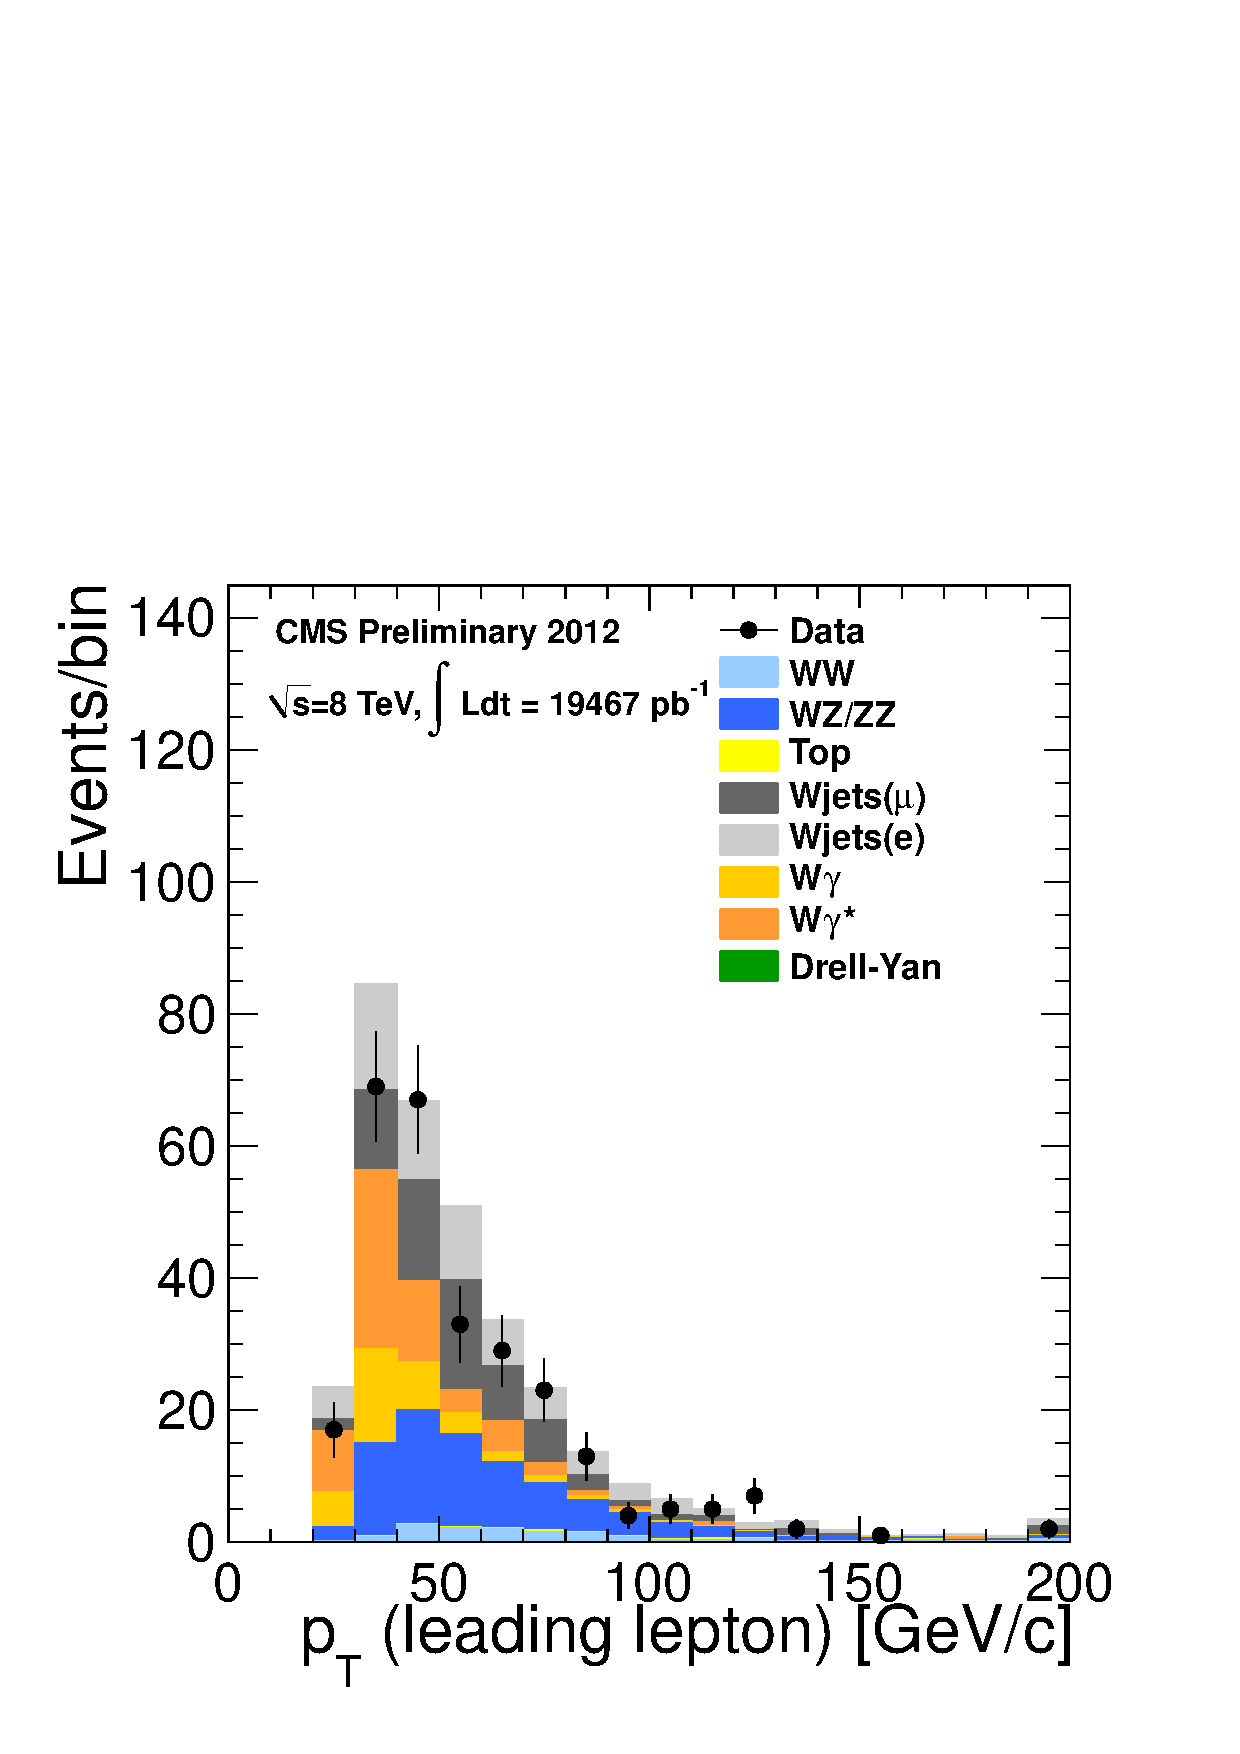
\includegraphics[width=.31\textwidth]{figures/hww_analysis24_0_ALL_of_0j_pt1.pdf}
}
\subfigure[Trailing lepton $p_T$]{
\centering
\label{subfig:ptmin}
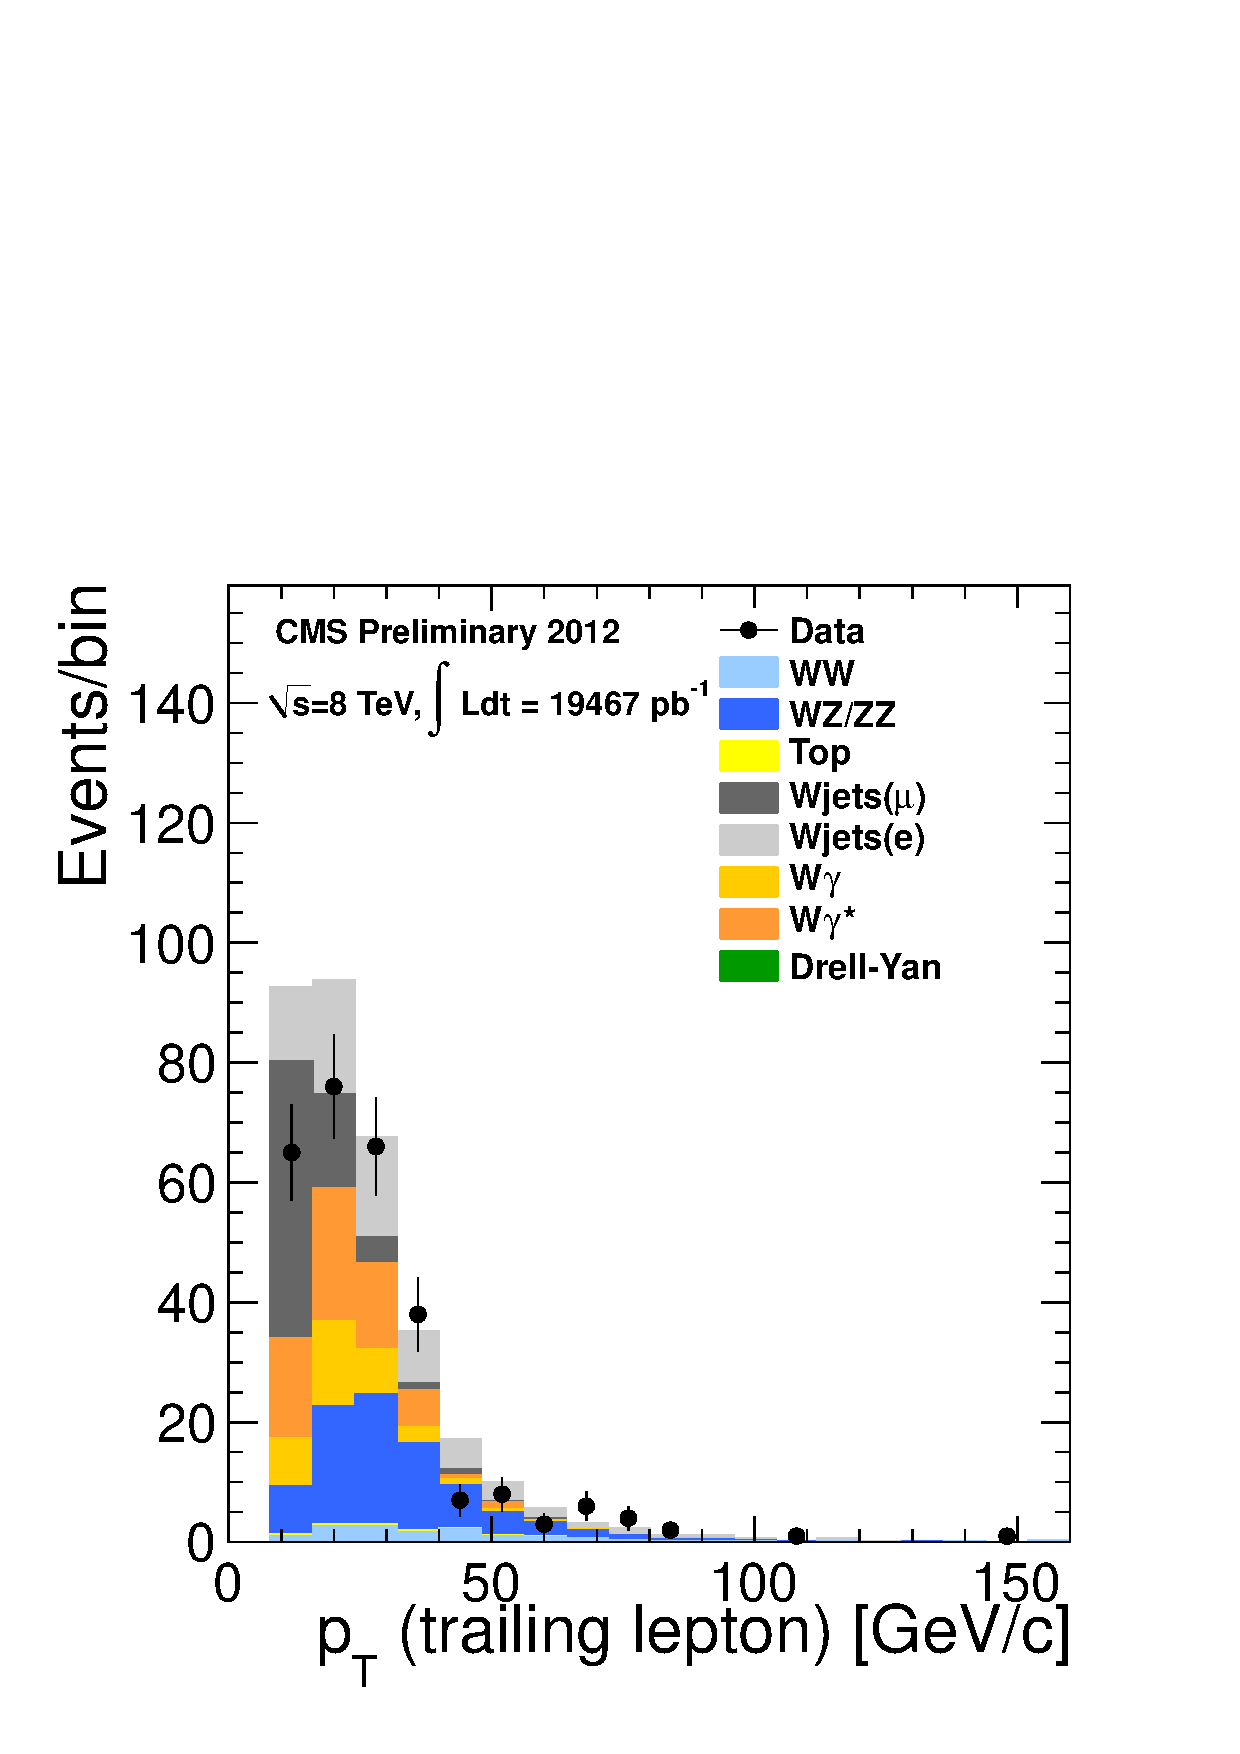
\includegraphics[width=.31\textwidth]{figures/hww_analysis24_0_ALL_of_0j_pt2.pdf}
}
\subfigure[Dilepton mass]{
\centering
\label{subfig:mll}
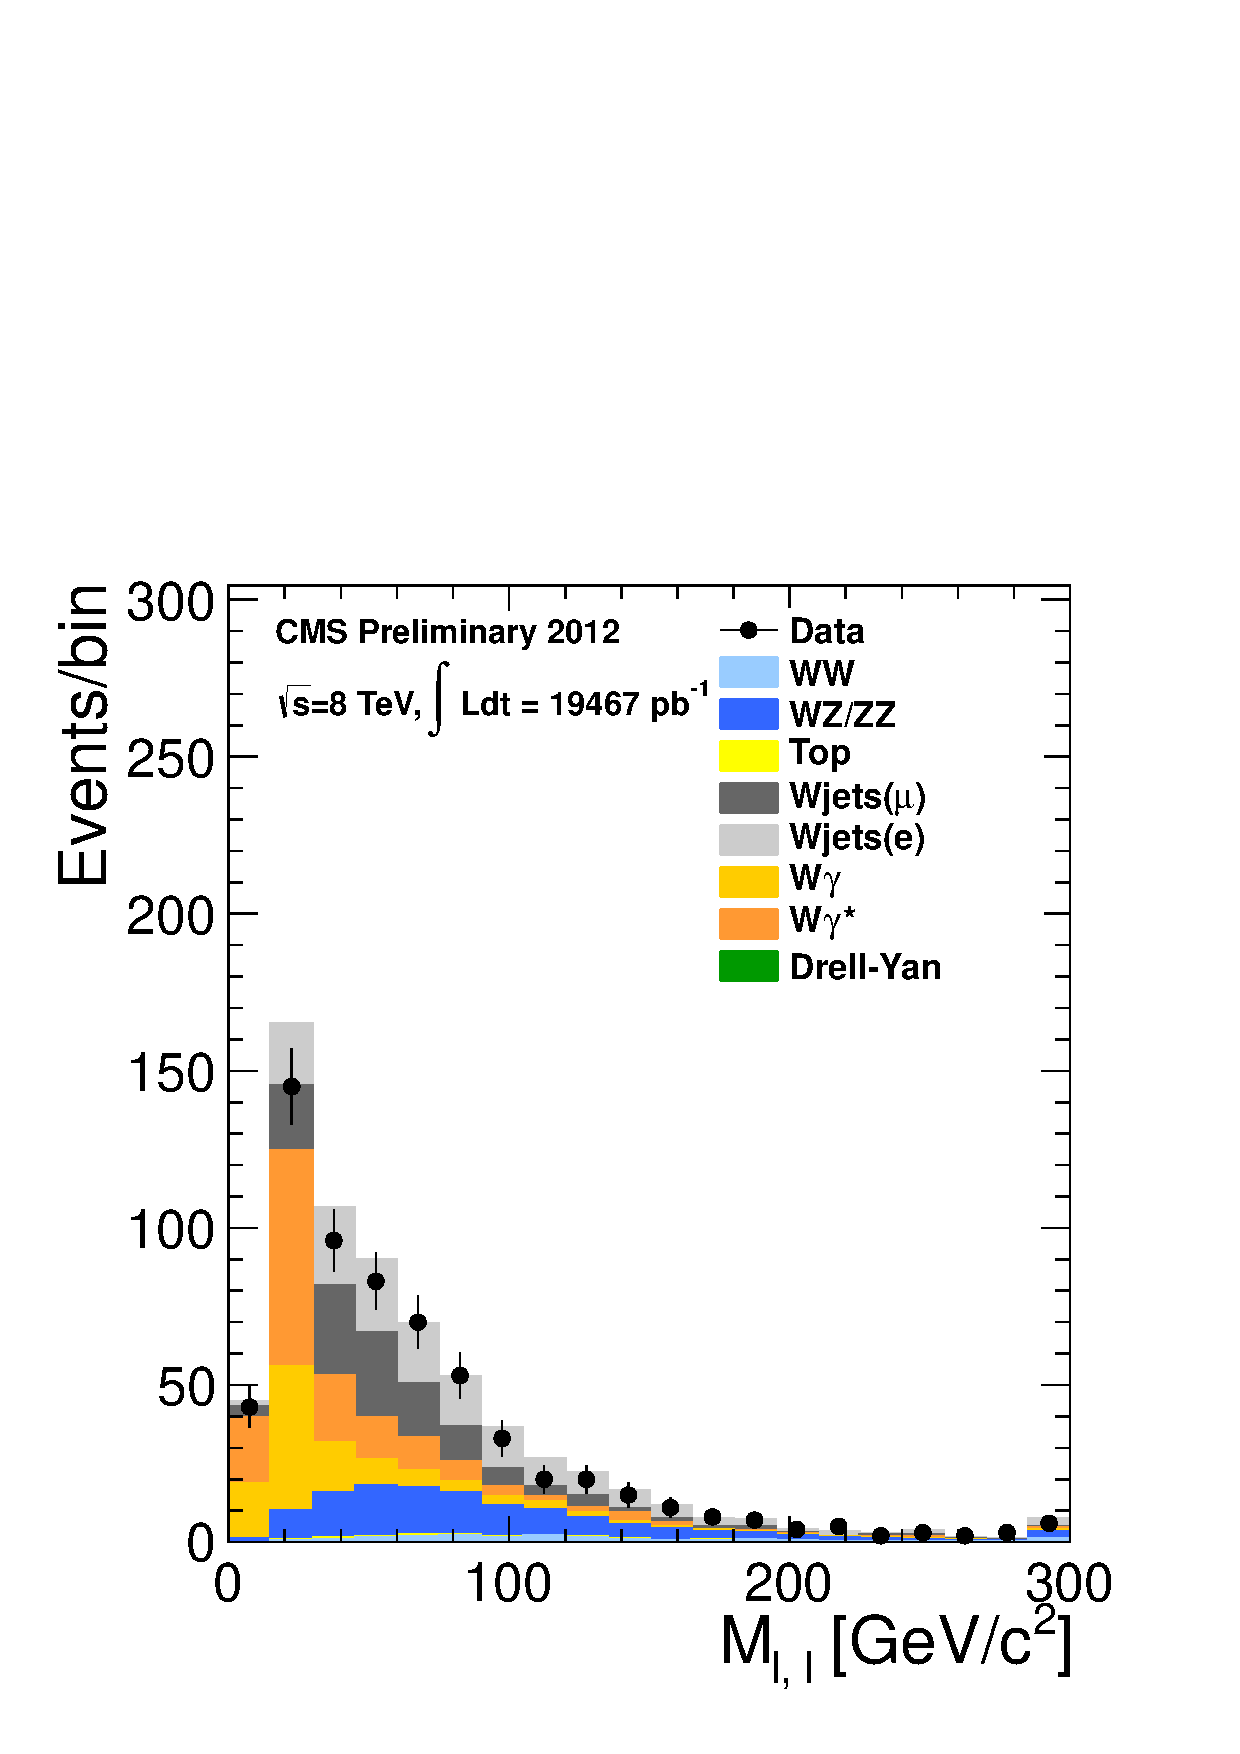
\includegraphics[width=.31\textwidth]{figures/hww_analysis24_0_ALL_of_0j_mll.pdf}
} \\
\subfigure[$\Delta\phi(\ell,\ell)$]{
\centering
\label{subfig:dphi}
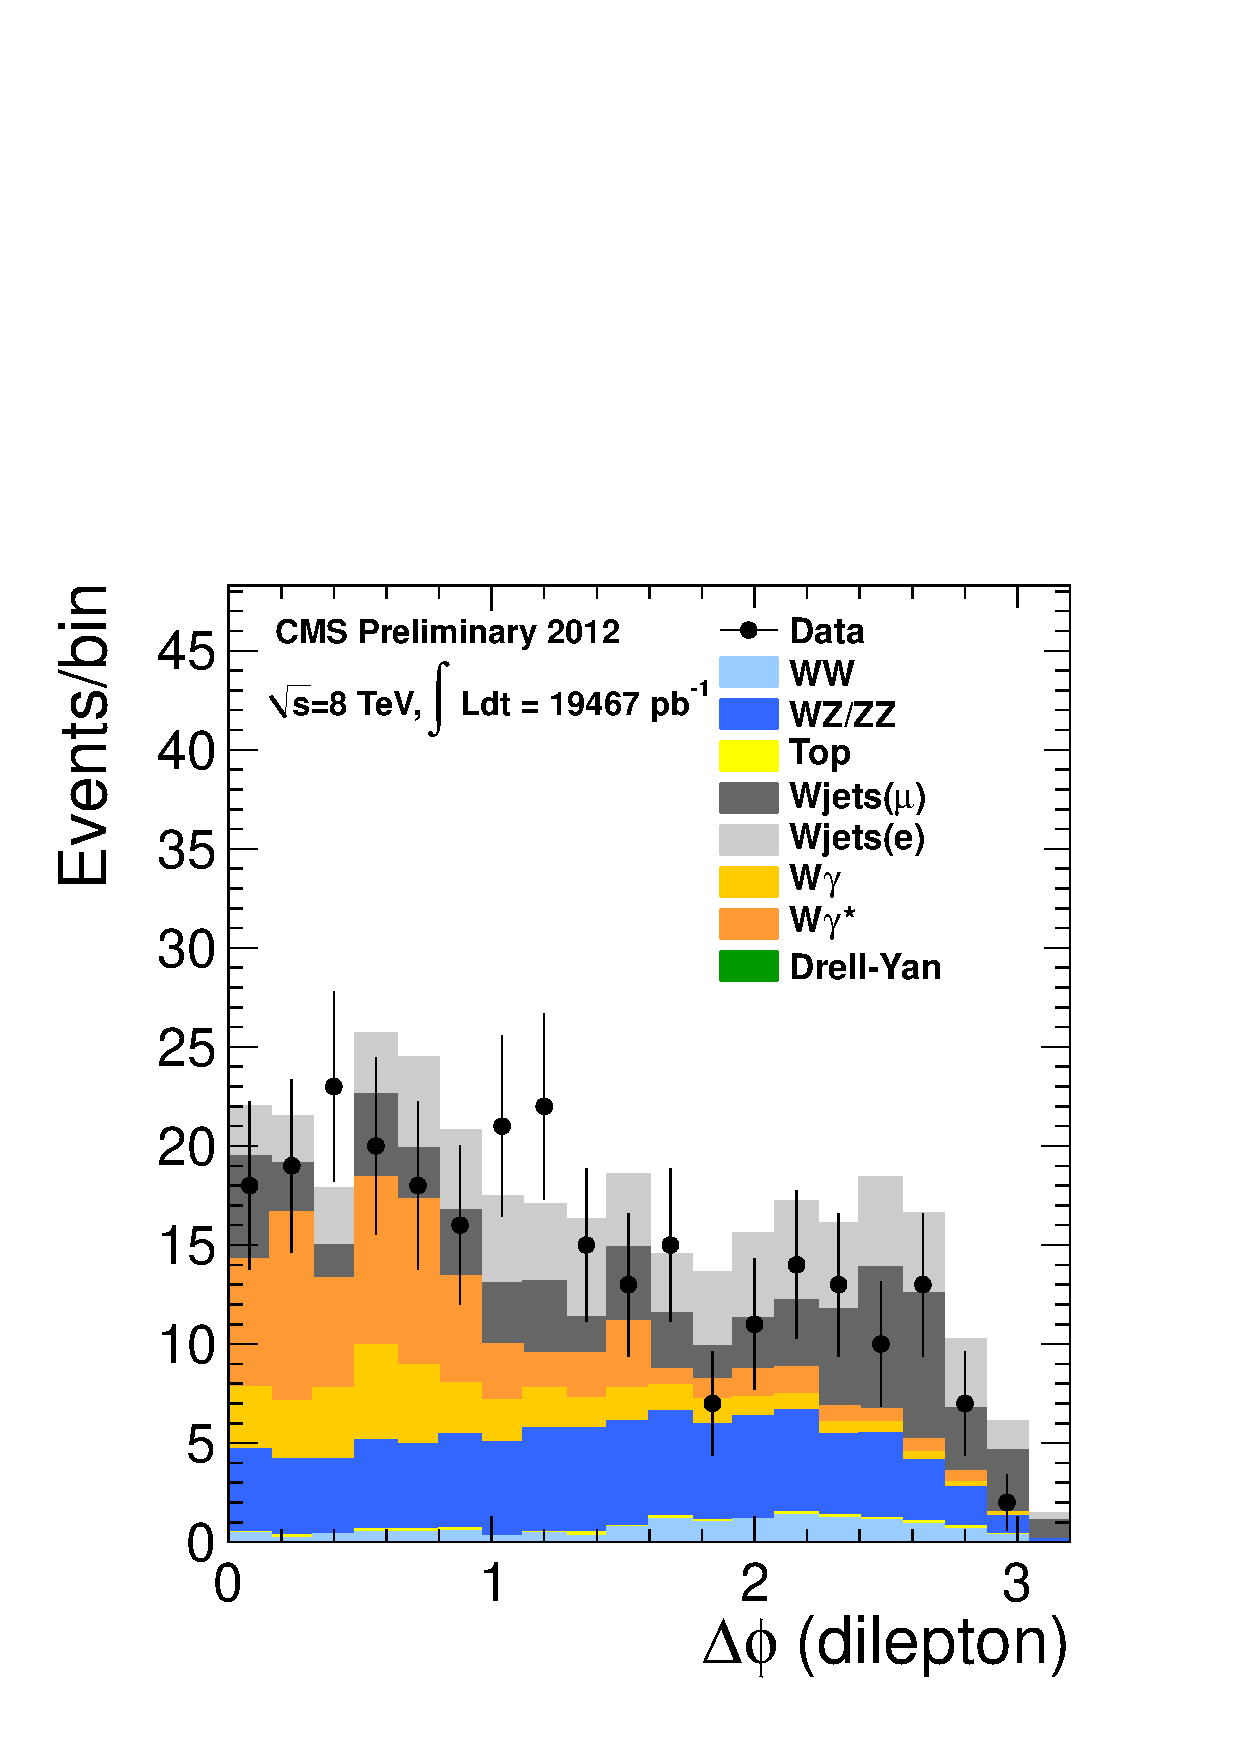
\includegraphics[width=.31\textwidth]{figures/hww_analysis24_0_ALL_of_0j_dphi.pdf}
}
\subfigure[MET]{
\centering
\label{subfig:ptmax}
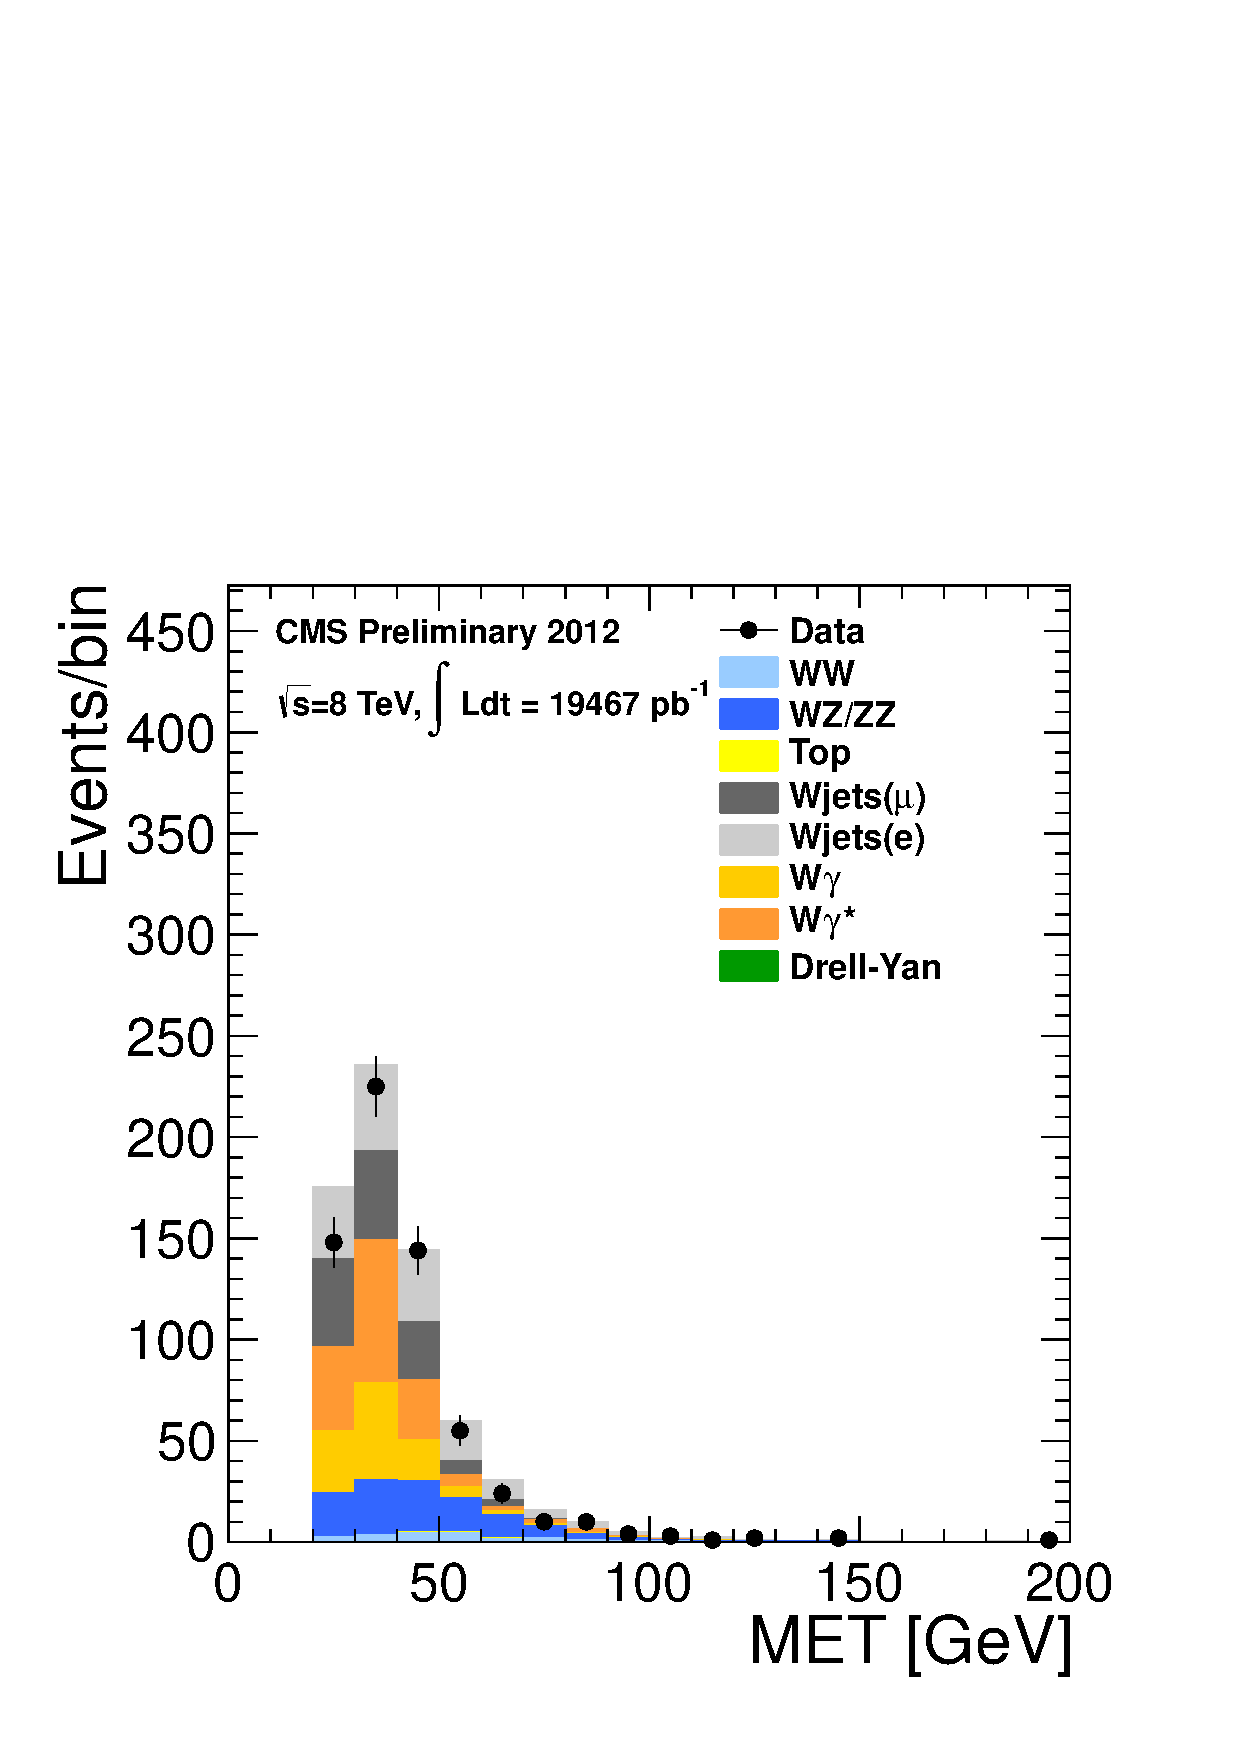
\includegraphics[width=.31\textwidth]{figures/hww_analysis24_0_ALL_of_0j_met.pdf}
}
\subfigure[Transverse Higgs Mass]{
\centering
\label{subfig:ptmin}
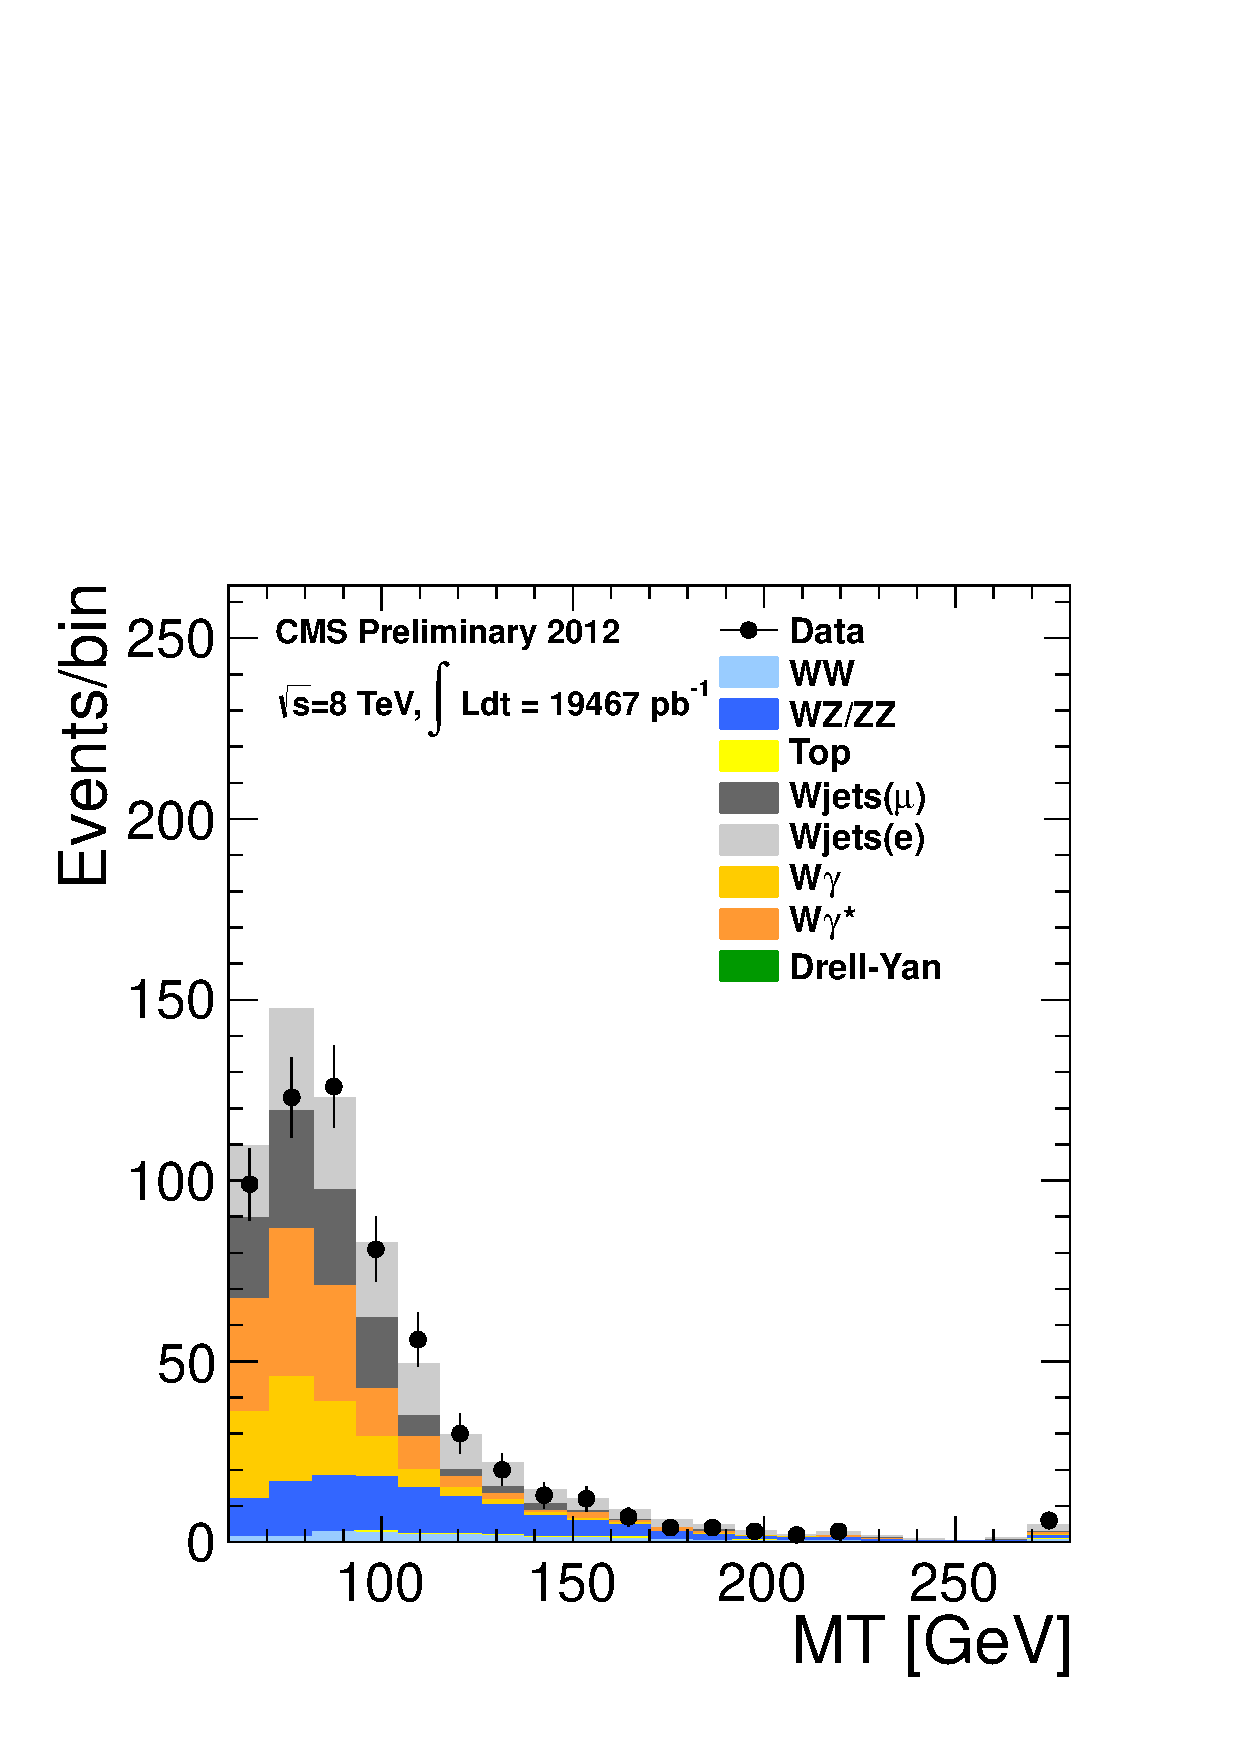
\includegraphics[width=.31\textwidth]{figures/hww_analysis24_0_ALL_of_0j_mt.pdf}
}\\

\caption{Kinematic distributions of the different flavor same sign events in 0-Jet bin. 
The WW preselections are applied.}
\label{fig:ssplots}
\end{figure}
%%%%%%%%%%%%%%%%%%%%%%%%%%%%%%

The top background estimation is shown in Table~\ref{tab:ttbar_est}. 
The scale factors are consistent with unity within 
the current large statistical uncertainties. 
Figure~\ref{fig:toptagplots} shows the kinematic distributions in the top enriched 
region. 

%%%%%%%%%%%%%%%%%%%%%%%%%%%%%%%%%%%%
\begin{figure}[!hbtp]
\centering
\subfigure[Leading lepton $p_T$]{
\centering
\label{subfig:ptmax}
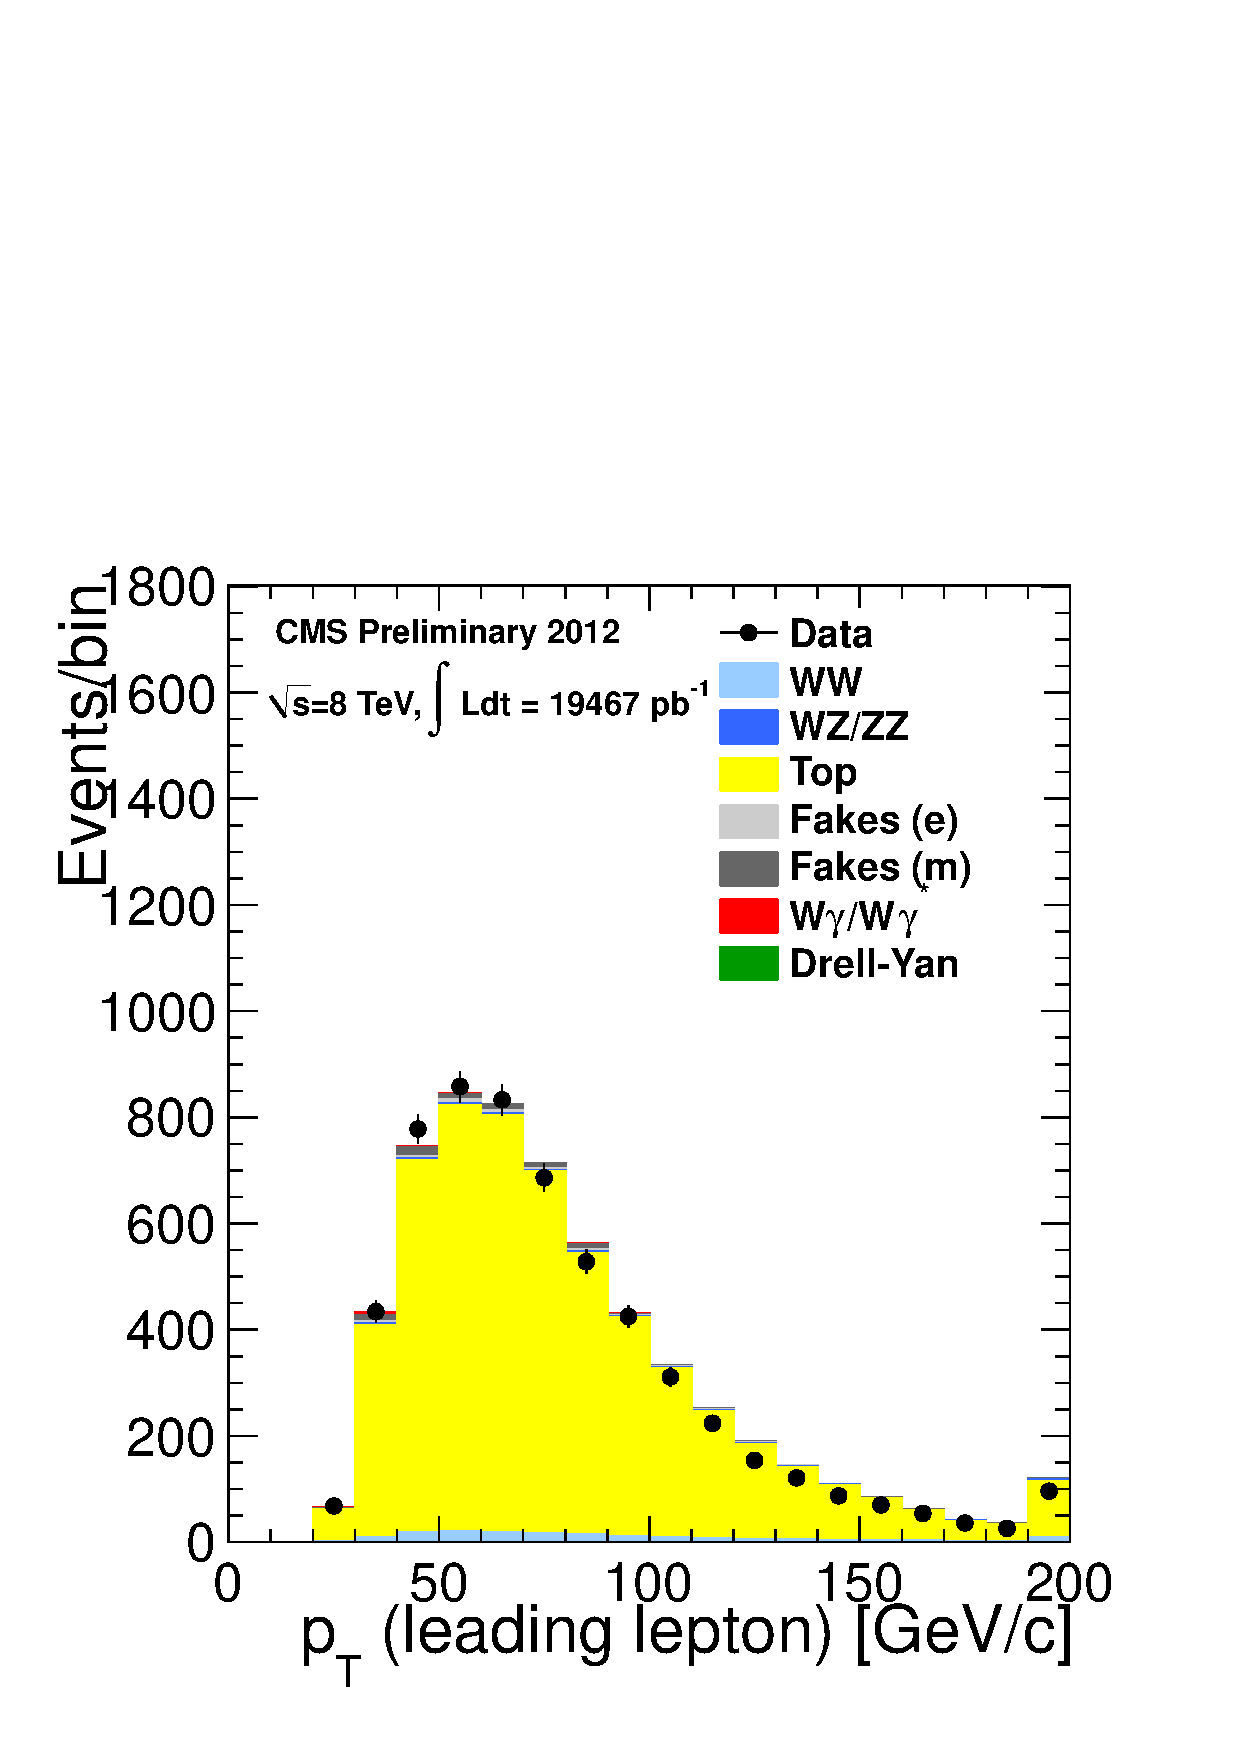
\includegraphics[width=.31\textwidth]{figures/hww_analysis16_0_ALL_of_1j_pt1_toptag.pdf}
}
\subfigure[Trailing lepton $p_T$]{
\centering
\label{subfig:ptmin}
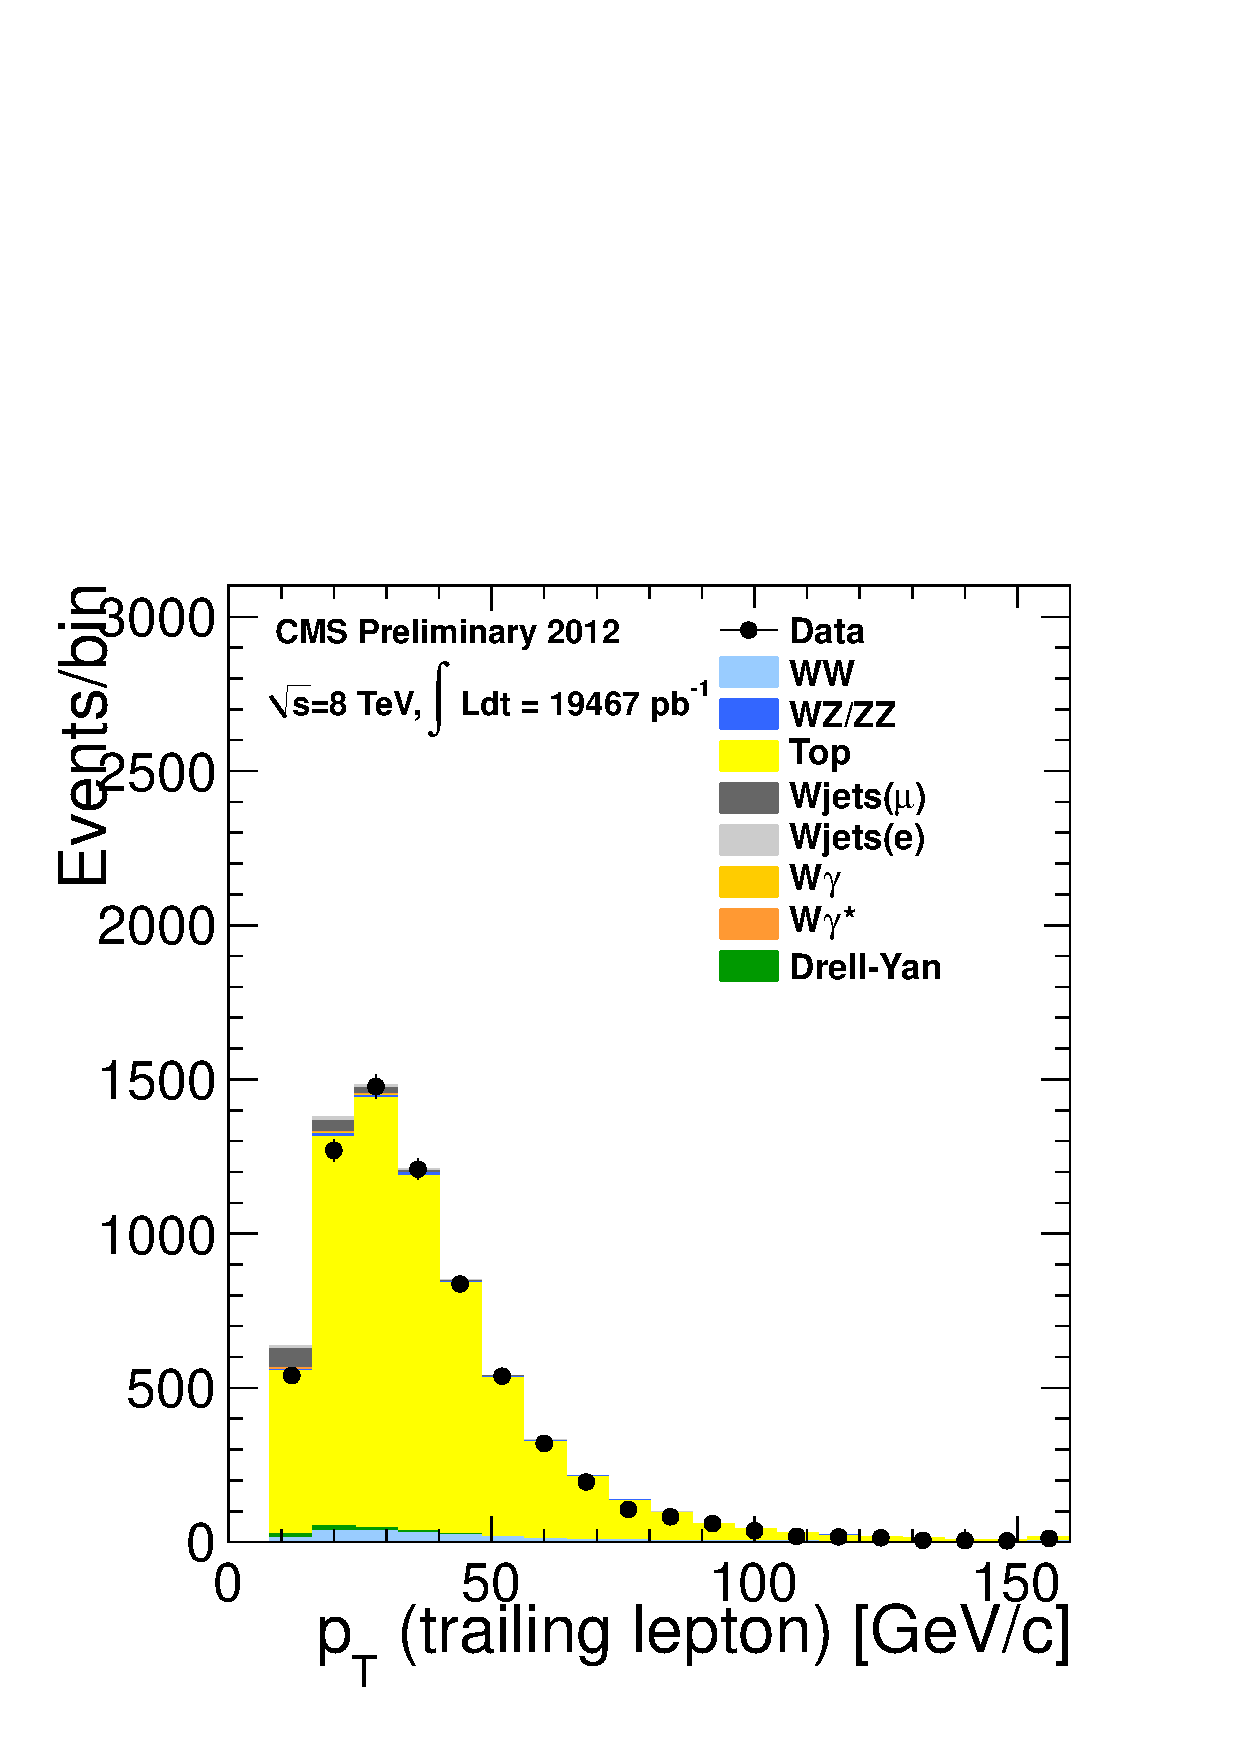
\includegraphics[width=.31\textwidth]{figures/hww_analysis16_0_ALL_of_1j_pt2_toptag.pdf}
}
\subfigure[Dilepton mass]{
\centering
\label{subfig:mll}
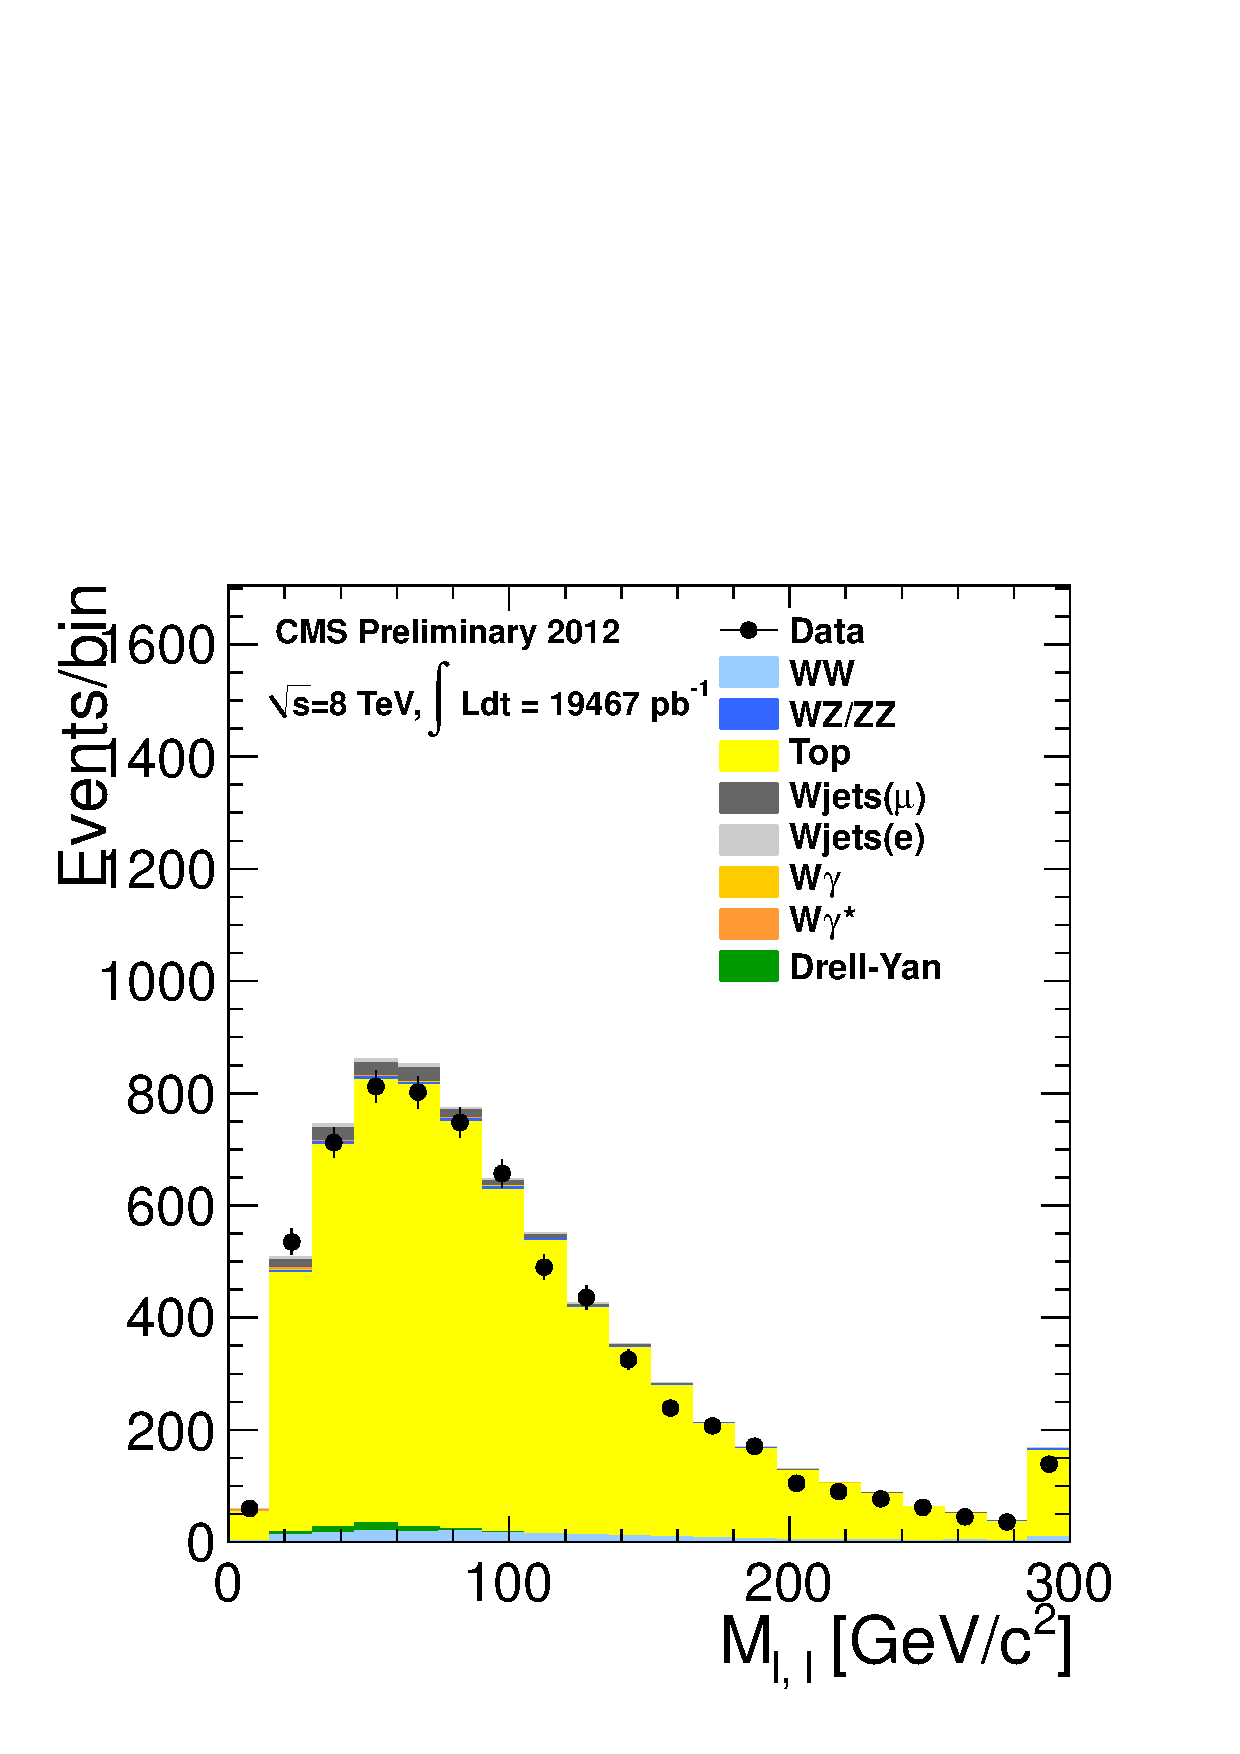
\includegraphics[width=.31\textwidth]{figures/hww_analysis16_0_ALL_of_1j_mll_toptag.pdf}
} \\
\subfigure[$\Delta\phi(\ell,\ell)$]{
\centering
\label{subfig:dphi}
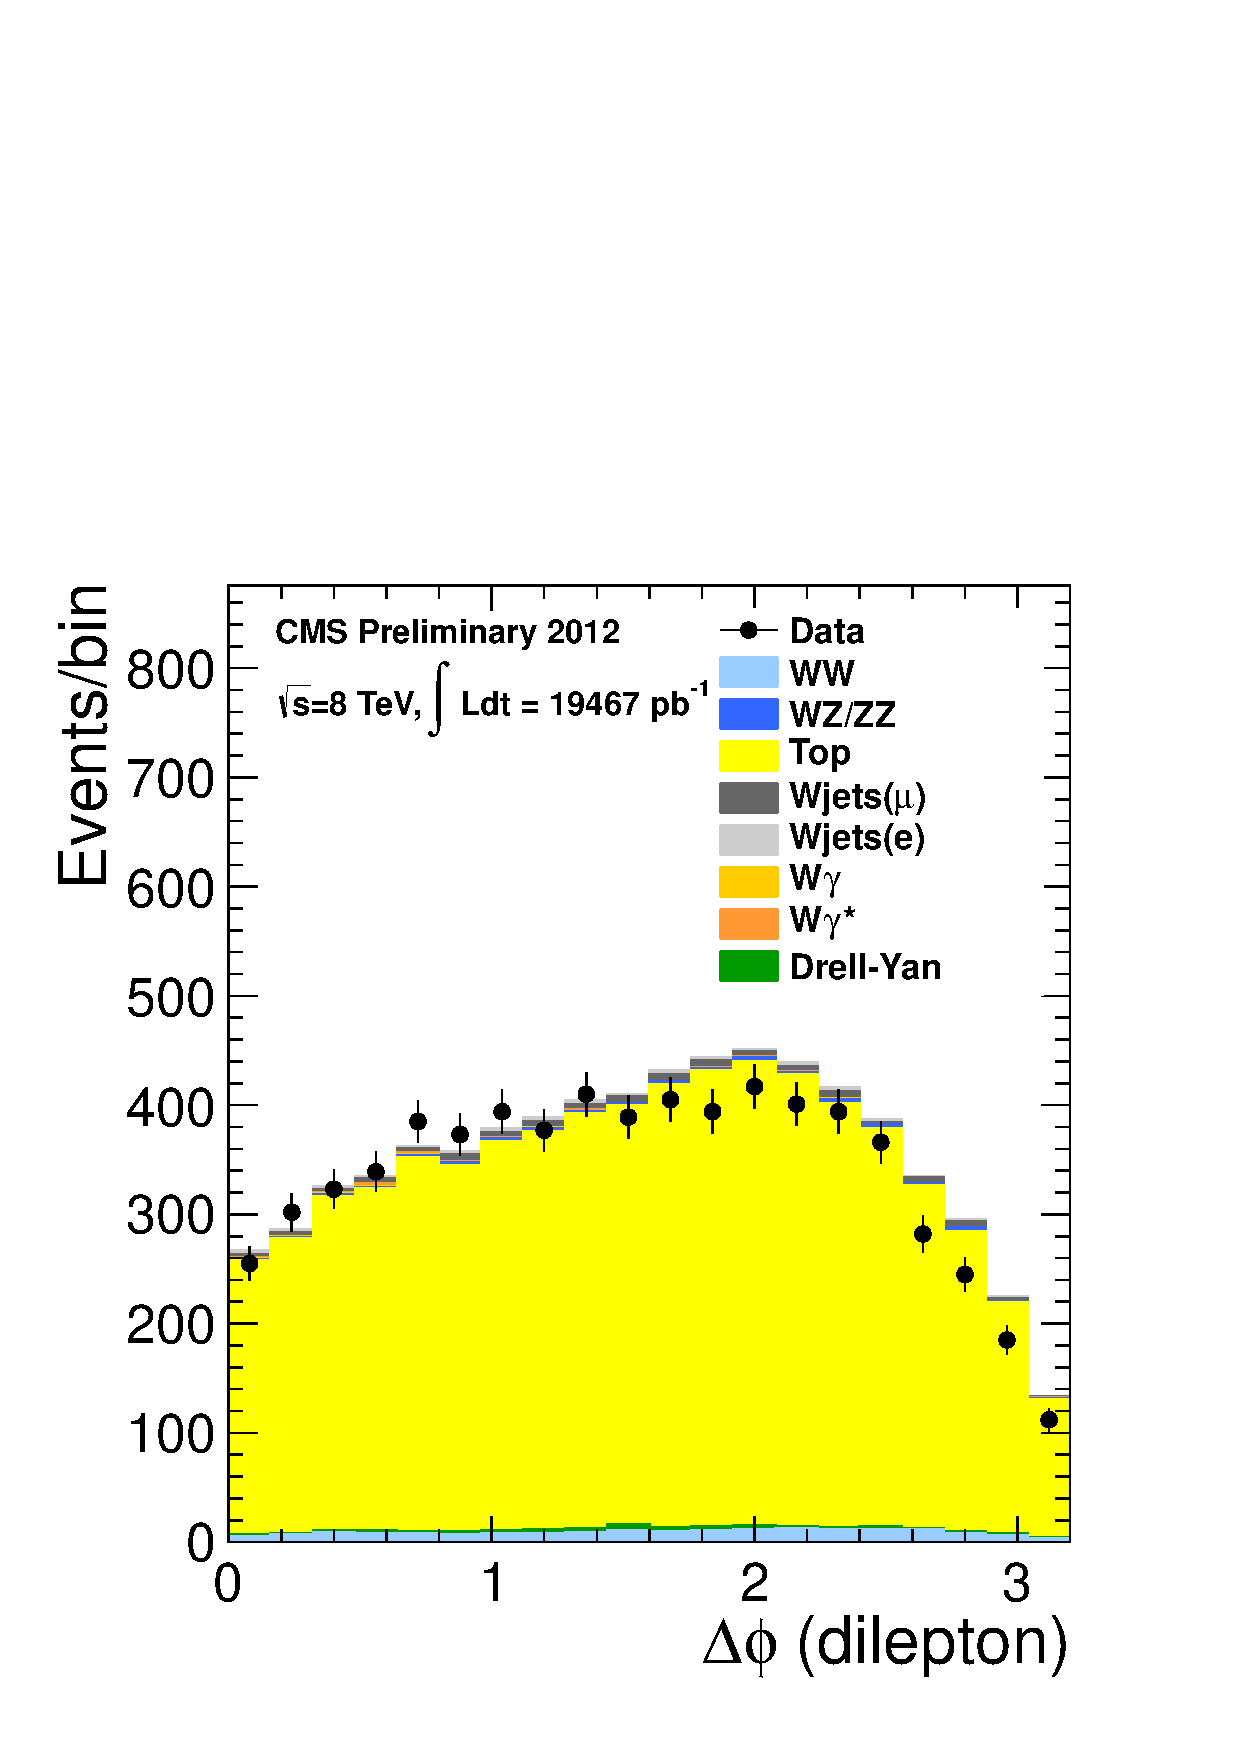
\includegraphics[width=.31\textwidth]{figures/hww_analysis16_0_ALL_of_1j_dphi_toptag.pdf}
}
\subfigure[MET]{
\centering
\label{subfig:ptmax}
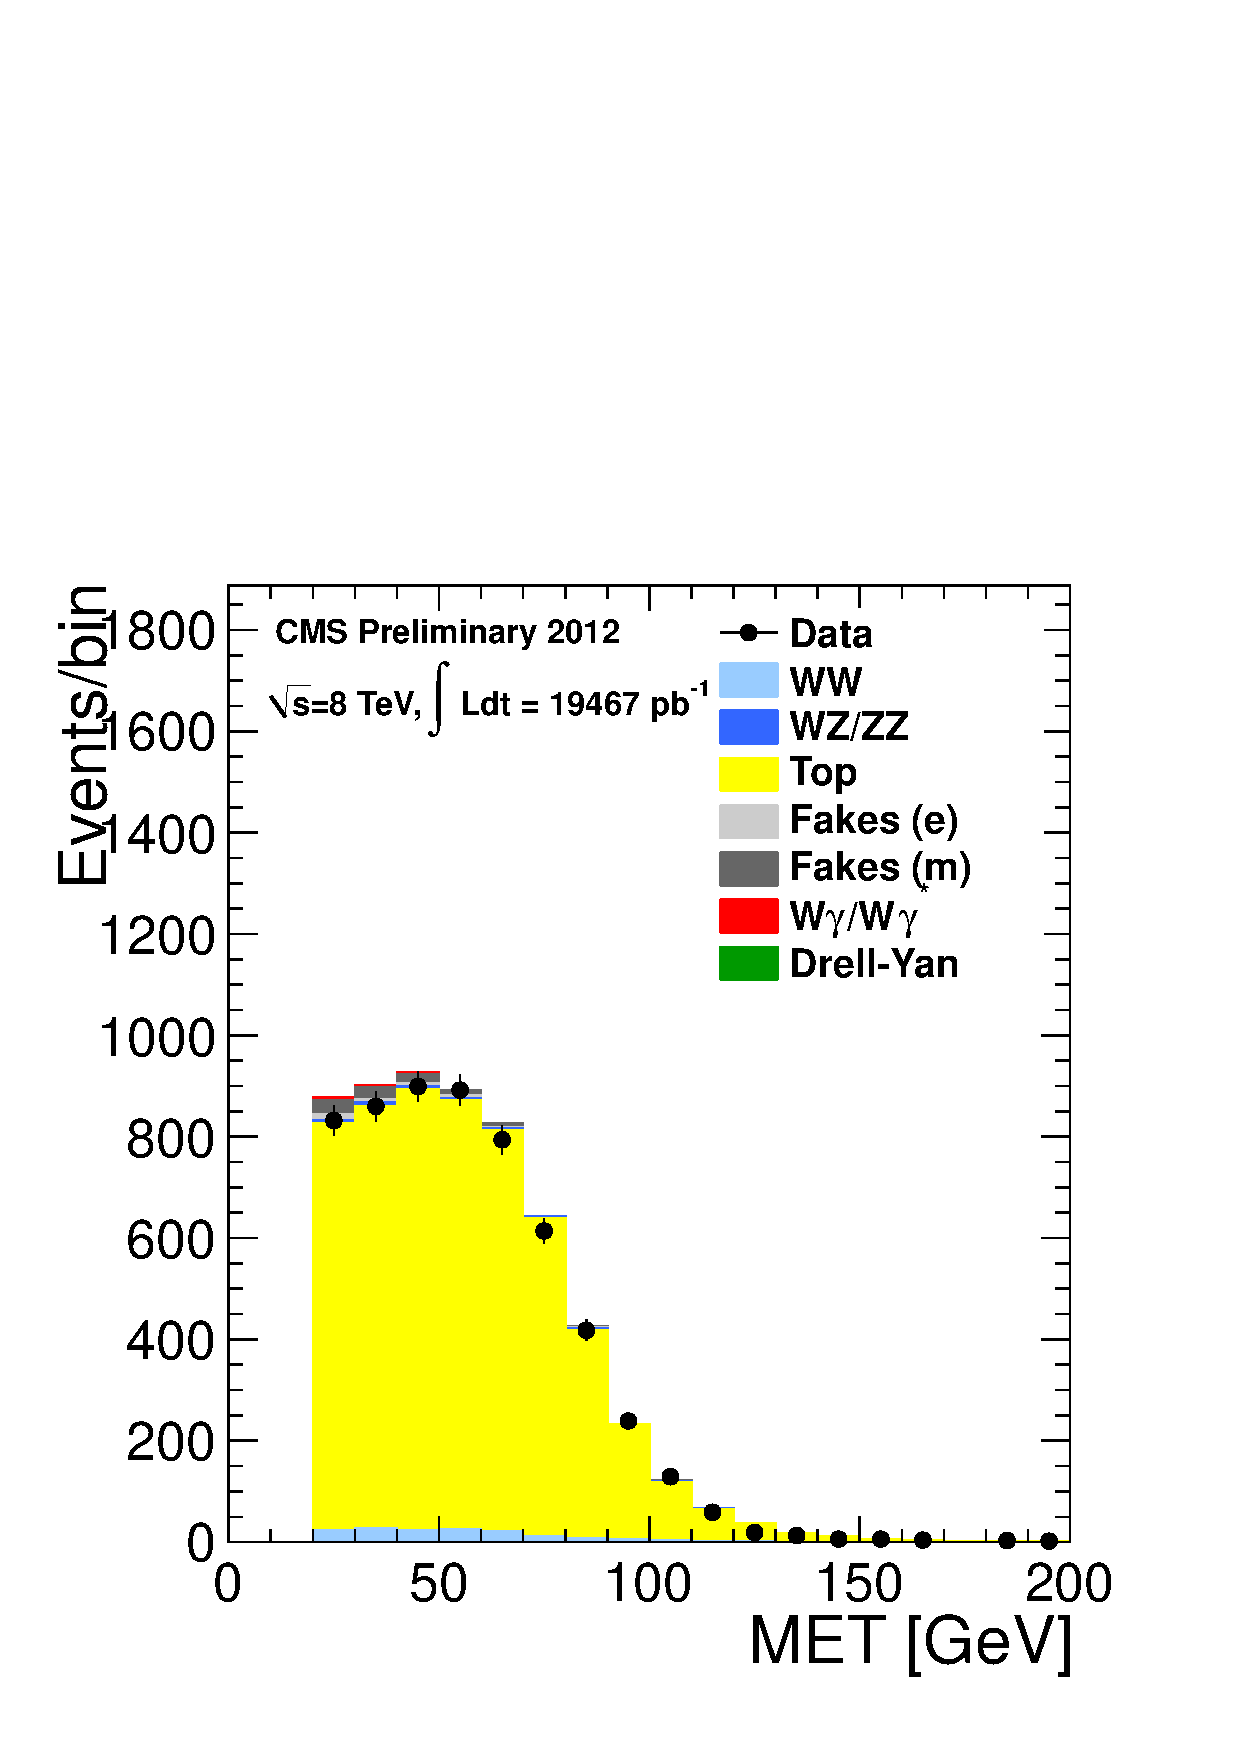
\includegraphics[width=.31\textwidth]{figures/hww_analysis16_0_ALL_of_1j_met_toptag.pdf}
}
\subfigure[Transverse Higgs Mass]{
\centering
\label{subfig:ptmin}
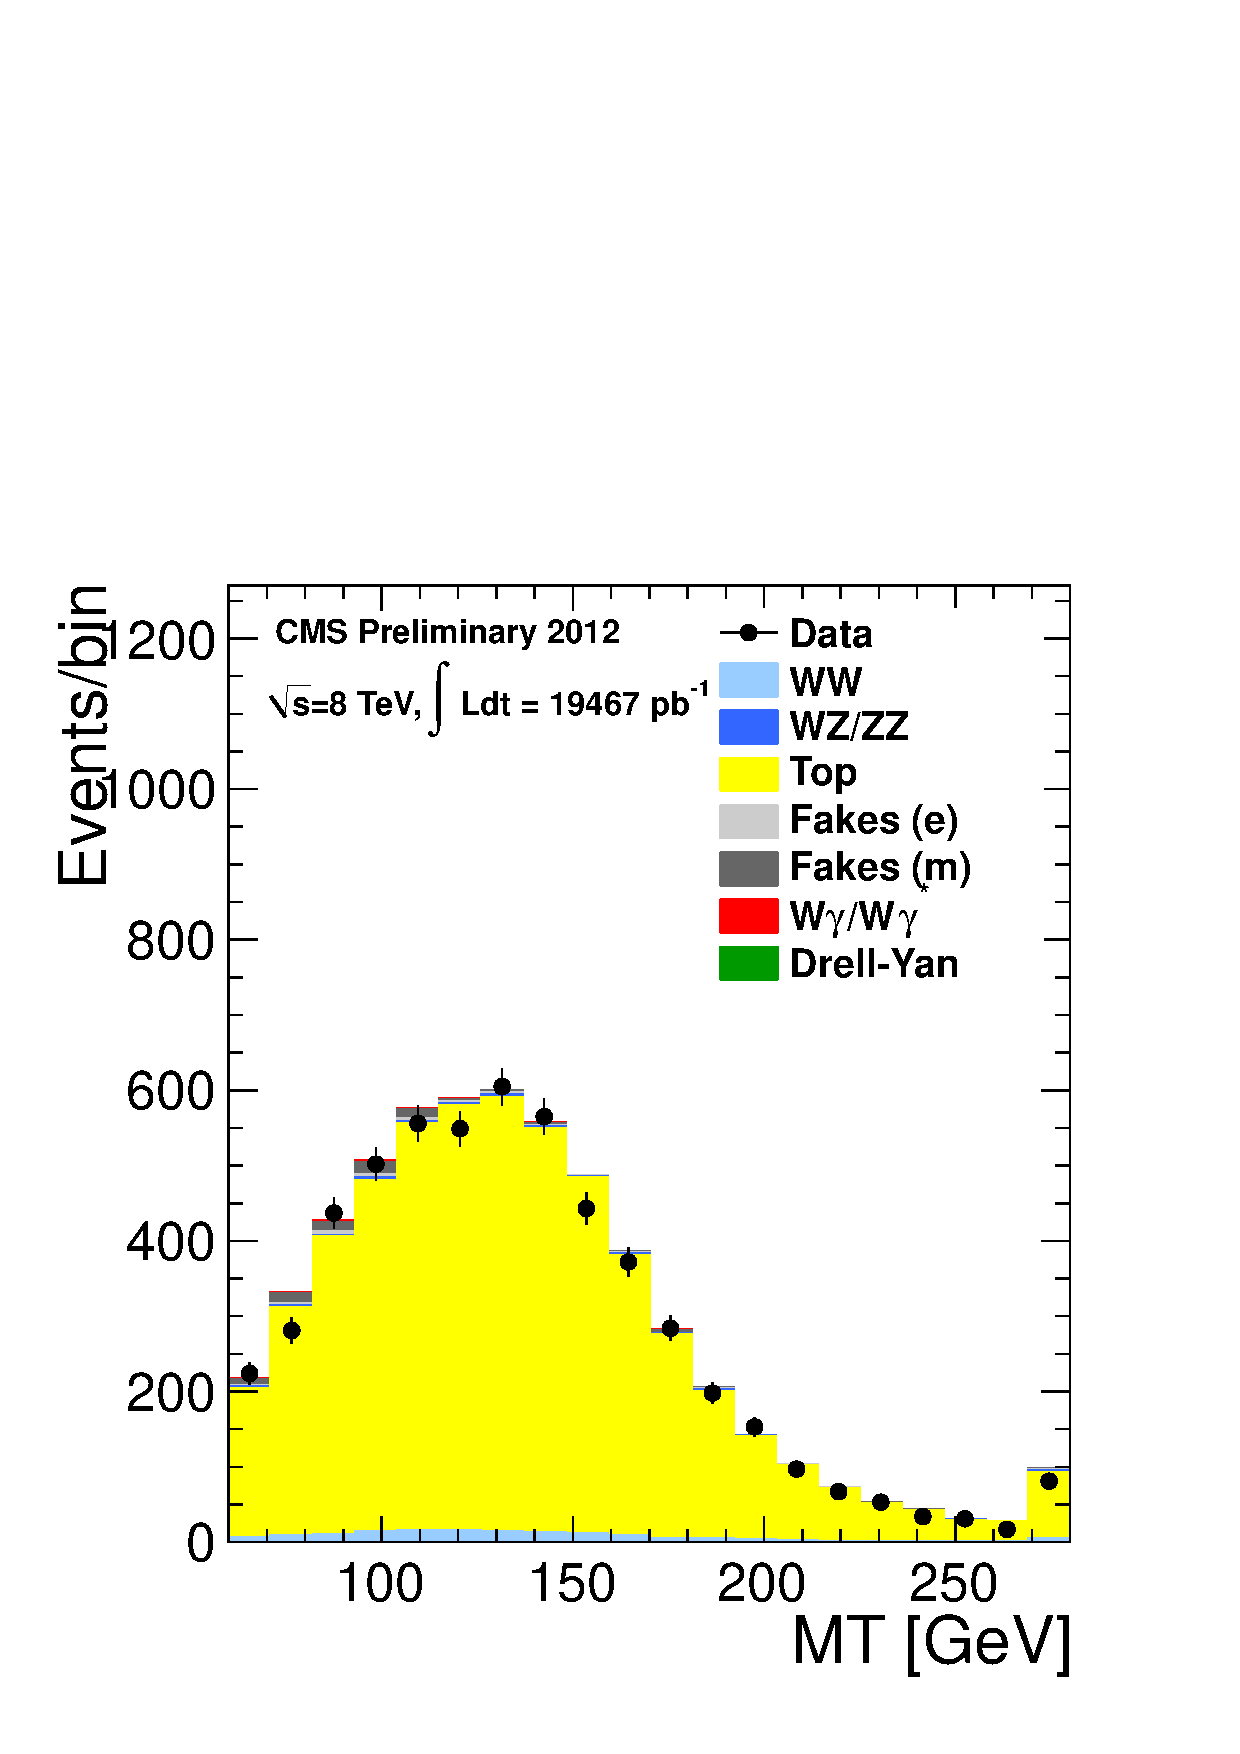
\includegraphics[width=.31\textwidth]{figures/hww_analysis16_0_ALL_of_1j_mt_toptag.pdf}
}\\
\caption{Kinematic distributions of the different flavor events in the 1-Jet bin in the Top enriched region.
We apply the WW selection inverting the Top veto requirements.}
\label{fig:toptagplots}
\end{figure}
%%%%%%%%%%%%%%%%%%%%%%%%%%%%%% 




With these results, we compare the yields after the $\WW$ preselection 
in data and MC(Table~\ref{tab:wwselection_all}). 
Higgs contribution at \WW\ selection level is negligible for not excluded Higgs mass
hypotheses. For the signal extraction we estimate the \WW\ background
contribution in data looking at events with large di-lepton mass, i.e.
$m_{ll}>100$~\GeV{} (Table~\ref{tab:ww_est}). 
Figures~\ref{fig:ww_ptmax}-\ref{fig:ww_deltaphi} show a few key distributions 
in $e\mu$ final states at \WW\ selection level.

%%%%%%%%%%%%%%%%%%%%%%%%%%%%%% 
\begin{table}
\begin{center}
\begin{tabular}{c c c c c c}
\hline
       nJets & $N_{in}$(data)        & $R_{out/in}$        & $N_{out}$(data)  & $N_{out}$ (MC) \\ 
\hline
0 & $775.16\pm74.47$ & $0.28\pm0.01\pm0.08$ & $218.64\pm21.53\pm65.59$ & $34.64\pm9.56$ \\
1 & $350.69\pm38.00$ & $0.25\pm0.01\pm0.08$ & $89.20\pm9.83\pm26.76$ & $21.05\pm7.16$ \\
\hline
\end{tabular}
\caption{The Drell-Yan estimation in the same flavor final state at WW preselection level, using the DYMVA.}
\label{tab:dy_wwlevel}
\end{center}
\end{table}

%%%%%%%%%%%%%%%%%%%%%%%%%%%%%%
\begin{table}
\begin{center}
\begin{tabular}{c c c c c c}
\hline
\hline
\multicolumn{5}{c}{0-jet} \\
\hline
mass & $N_{in}$(data)        & $R_{out/in}$        & $N_{out}$(data)  & $N_{out}$ (MC) \\ 
\hline
\vspace{-3mm}  \\
115 \GeV & $145.94\pm15.08$ & $0.31\pm0.01\pm0.09$ & $45.07\pm4.81\pm13.52$ & $8.70\pm5.08$ \\
120 \GeV & $263.31\pm20.83$ & $0.31\pm0.01\pm0.09$ & $81.33\pm6.80\pm24.40$ & $13.57\pm5.88$ \\
125 \GeV & $154.60\pm16.13$ & $0.60\pm0.02\pm0.19$ & $92.22\pm9.98\pm29.33$ & $16.64\pm6.63$ \\
130 \GeV & $119.10\pm14.17$ & $0.87\pm0.03\pm0.26$ & $103.61\pm12.74\pm31.08$ & $16.64\pm6.63$ \\
135 \GeV & $112.30\pm14.57$ & $0.83\pm0.03\pm0.25$ & $93.52\pm12.49\pm28.06$ & $14.53\pm6.29$ \\
140 \GeV & $108.72\pm14.48$ & $0.74\pm0.02\pm0.22$ & $80.72\pm11.09\pm24.22$ & $17.17\pm6.82$ \\
150 \GeV & $91.78\pm14.57$ & $0.40\pm0.02\pm0.12$ & $37.01\pm6.20\pm11.10$ & $7.60\pm4.47$ \\
160 \GeV & $21.03\pm8.64$ & $0.90\pm0.06\pm0.27$ & $18.83\pm7.85\pm5.65$ & $7.60\pm4.47$ \\
170 \GeV & $9.70\pm8.14$ & $0.82\pm0.06\pm0.25$ & $7.92\pm6.68\pm2.38$ & $7.60\pm4.47$ \\
180 \GeV & $7.06\pm9.35$ & $0.62\pm0.05\pm0.19$ & $4.34\pm5.76\pm1.34$ & $5.71\pm4.05$ \\
190 \GeV & $64.23\pm15.78$ & $0.34\pm0.02\pm0.10$ & $21.63\pm5.51\pm6.49$ & $10.31\pm5.20$ \\
200 \GeV & $94.35\pm21.88$ & $0.21\pm0.01\pm0.06$ & $20.10\pm4.83\pm6.03$ & $7.67\pm4.47$ \\
250 \GeV & $193.85\pm36.84$ & $0.06\pm0.00\pm0.02$ & $11.17\pm2.24\pm3.35$ & $7.08\pm4.09$ \\
300 \GeV & $89.23\pm27.97$ & $0.13\pm0.01\pm0.04$ & $11.16\pm3.62\pm3.35$ & $7.08\pm4.09$ \\
\hline
\hline
\multicolumn{5}{c}{1-jet} \\
\hline
mass & $N_{in}$(data)        & $R_{out/in}$        & $N_{out}$(data)  & $N_{out}$ (MC) \\ 
\hline
\vspace{-3mm}  \\
115 \GeV & $28.00\pm8.66$ & $0.19\pm0.00\pm0.06$ & $5.28\pm1.64\pm1.58$ & $2.16\pm2.16$ \\
120 \GeV & $71.36\pm12.41$ & $0.19\pm0.00\pm0.06$ & $13.45\pm2.36\pm4.04$ & $4.35\pm3.08$ \\
125 \GeV & $53.67\pm10.57$ & $0.27\pm0.01\pm0.08$ & $14.69\pm2.92\pm4.41$ & $4.35\pm3.08$ \\
130 \GeV & $39.38\pm9.49$ & $0.36\pm0.01\pm0.11$ & $14.21\pm3.44\pm4.26$ & $4.35\pm3.08$ \\
135 \GeV & $45.07\pm9.97$ & $0.34\pm0.01\pm0.10$ & $15.32\pm3.41\pm4.60$ & $4.35\pm3.08$ \\
140 \GeV & $46.46\pm10.18$ & $0.31\pm0.01\pm0.09$ & $14.32\pm3.16\pm4.30$ & $4.35\pm3.08$ \\
150 \GeV & $59.54\pm12.09$ & $0.20\pm0.01\pm0.06$ & $11.79\pm2.43\pm3.54$ & $2.19\pm2.19$ \\
160 \GeV & $20.90\pm6.94$ & $0.42\pm0.02\pm0.13$ & $8.80\pm2.95\pm2.64$ & $0.00\pm0.00$ \\
170 \GeV & $16.48\pm6.89$ & $0.39\pm0.02\pm0.12$ & $6.49\pm2.73\pm1.95$ & $0.00\pm0.00$ \\
180 \GeV & $22.86\pm8.18$ & $0.33\pm0.01\pm0.10$ & $7.51\pm2.71\pm2.25$ & $0.00\pm0.00$ \\
190 \GeV & $70.87\pm13.43$ & $0.22\pm0.01\pm0.07$ & $15.71\pm3.04\pm4.71$ & $0.00\pm0.00$ \\
200 \GeV & $99.31\pm16.50$ & $0.17\pm0.01\pm0.05$ & $16.60\pm2.83\pm4.98$ & $0.00\pm0.00$ \\
250 \GeV & $128.66\pm21.79$ & $0.09\pm0.00\pm0.03$ & $12.08\pm2.11\pm3.63$ & $2.65\pm2.65$ \\
300 \GeV & $71.21\pm17.81$ & $0.11\pm0.01\pm0.03$ & $7.94\pm2.03\pm2.38$ & $5.00\pm3.54$ \\
\hline
\end{tabular}
\caption{The Drell-Yan estimation in the same flavor final state, for the cut-based selections.}
\label{tab:dy}
\end{center}
\end{table}

%%%%%%%%%%%%%%%%%%%%%%%%%%%%%%
\begin{table}[ht!]
\begin{center}
\begin{tabular}{l c c}
\hline
                             Sample & 0-jet           	& 1-jet           	   	\\
\hline
estimated top events in simulation  & 720.5 $\pm$   4.3 &  2151.3 $\pm$  13.9    \\
tagging efficiency     (\%)         & 49.3 $\pm$  4.3 & 64.8 $\pm$  0.5          \\ 
data events in control region       & 1034 & 4847			         \\ 
background events in control region & 292.6 $\pm$  43.9 &  255.5 $\pm$  51.1     \\ 
top estimation in data              &  761.4 $\pm$ 146.5 &  2307.9 $\pm$  59.4   \\
data/simulation scale factor        &   1.06 $\pm$  0.20 &   1.07 $\pm$  0.03    \\
\hline

\hline
\end{tabular}
\caption{Monte Carlo to data scale factor for the top background contribution for $\intlumiEightTeV$. 
In the 1-jet bin, the scale factor is derived in a region that is slightly different from the signal region.}
\label{tab:ttbar_est}
\end{center}
\end{table}


%%%%%%%%%%%%%%%%%%%%%%%%%%%%%%%%%%%%
\begin{table}[ht!]
\begin{center}
\begin{tabular}{c|c|c|c|c}
\hline
\hline
                & SF-0j                 &  DF-0j              &           SF-1j     & DF-1j               \\
\hline
$qq \to \WW$    & 1782.4 $\pm$ 11.6	& 4402.1 $\pm$ 18.0 &  533.7 $\pm$  6.0  &  1414.3 $\pm$   9.7 \\
$gg \to \WW$    &  124.0 $\pm$  2.2	&  223.7 $\pm$  3.0 &	34.1 $\pm$  1.1  &    76.3 $\pm$   1.6 \\
$\ttbar+tW$     &  273.3 $\pm$  7.8	&  563.7 $\pm$ 11.1 &  677.2 $\pm$ 10.4  &  1644.2 $\pm$  16.8  \\
\wgamma         &   23.5 $\pm$  5.7	&  140.0 $\pm$ 16.9 &	11.9 $\pm$  4.8  &    51.8 $\pm$   9.2 \\
\Wgstar         &   13.7 $\pm$  2.0	&  147.9 $\pm$  6.5 &	 2.4 $\pm$  0.8  &    23.9 $\pm$   2.7 \\
VVV             &   19.8 $\pm$  1.0	&   38.3 $\pm$  1.4 &	16.3 $\pm$  1.5  &    33.4 $\pm$   1.7 \\
WZ              &   36.8 $\pm$  0.6	&  105.5 $\pm$  1.0 &	23.4 $\pm$  0.5  &   100.7 $\pm$   1.0 \\
$\Wjets$        &  107.5 $\pm$  4.6	&  694.8 $\pm$ 10.3 &	47.4 $\pm$  3.6  &   356.2 $\pm$   7.9 \\
$\Zjets$        &  294.6 $\pm$ 60.3	&   82.5 $\pm$  1.4 &  118.4 $\pm$ 30.3  &   248.7 $\pm$   2.8  \\
\hline
Total Bkg.      & 2676.3 $\pm$ 62.5     & 6399.1 $\pm$ 30.1 & 1465.3 $\pm$ 33.3 &   3950.0 $\pm$  23.7   \\
\hline
Data            & 2728                  & 6361                & 1477             & 3944    \\
\hline
\hline
\end{tabular}
  \caption{Expected number of signal and background events from the data-driven methods for 
  an integrated luminosity of \intlumiEightTeV after applying the $\WW$ selection requirements. 
  Only statistical uncertainties on the processes are reported.
  $\WW$ yield is from simulation.}
   \label{tab:wwselection_all}
\end{center}
\end{table}

%%%%%%%%%%%%%%%%%%%%%%%%%%%%%%%%%%%%
\begin{figure}[!hbtp]
\centering
\subfigure[0-Jet]{
\centering
\label{subfig:ww_ptmin_0j}
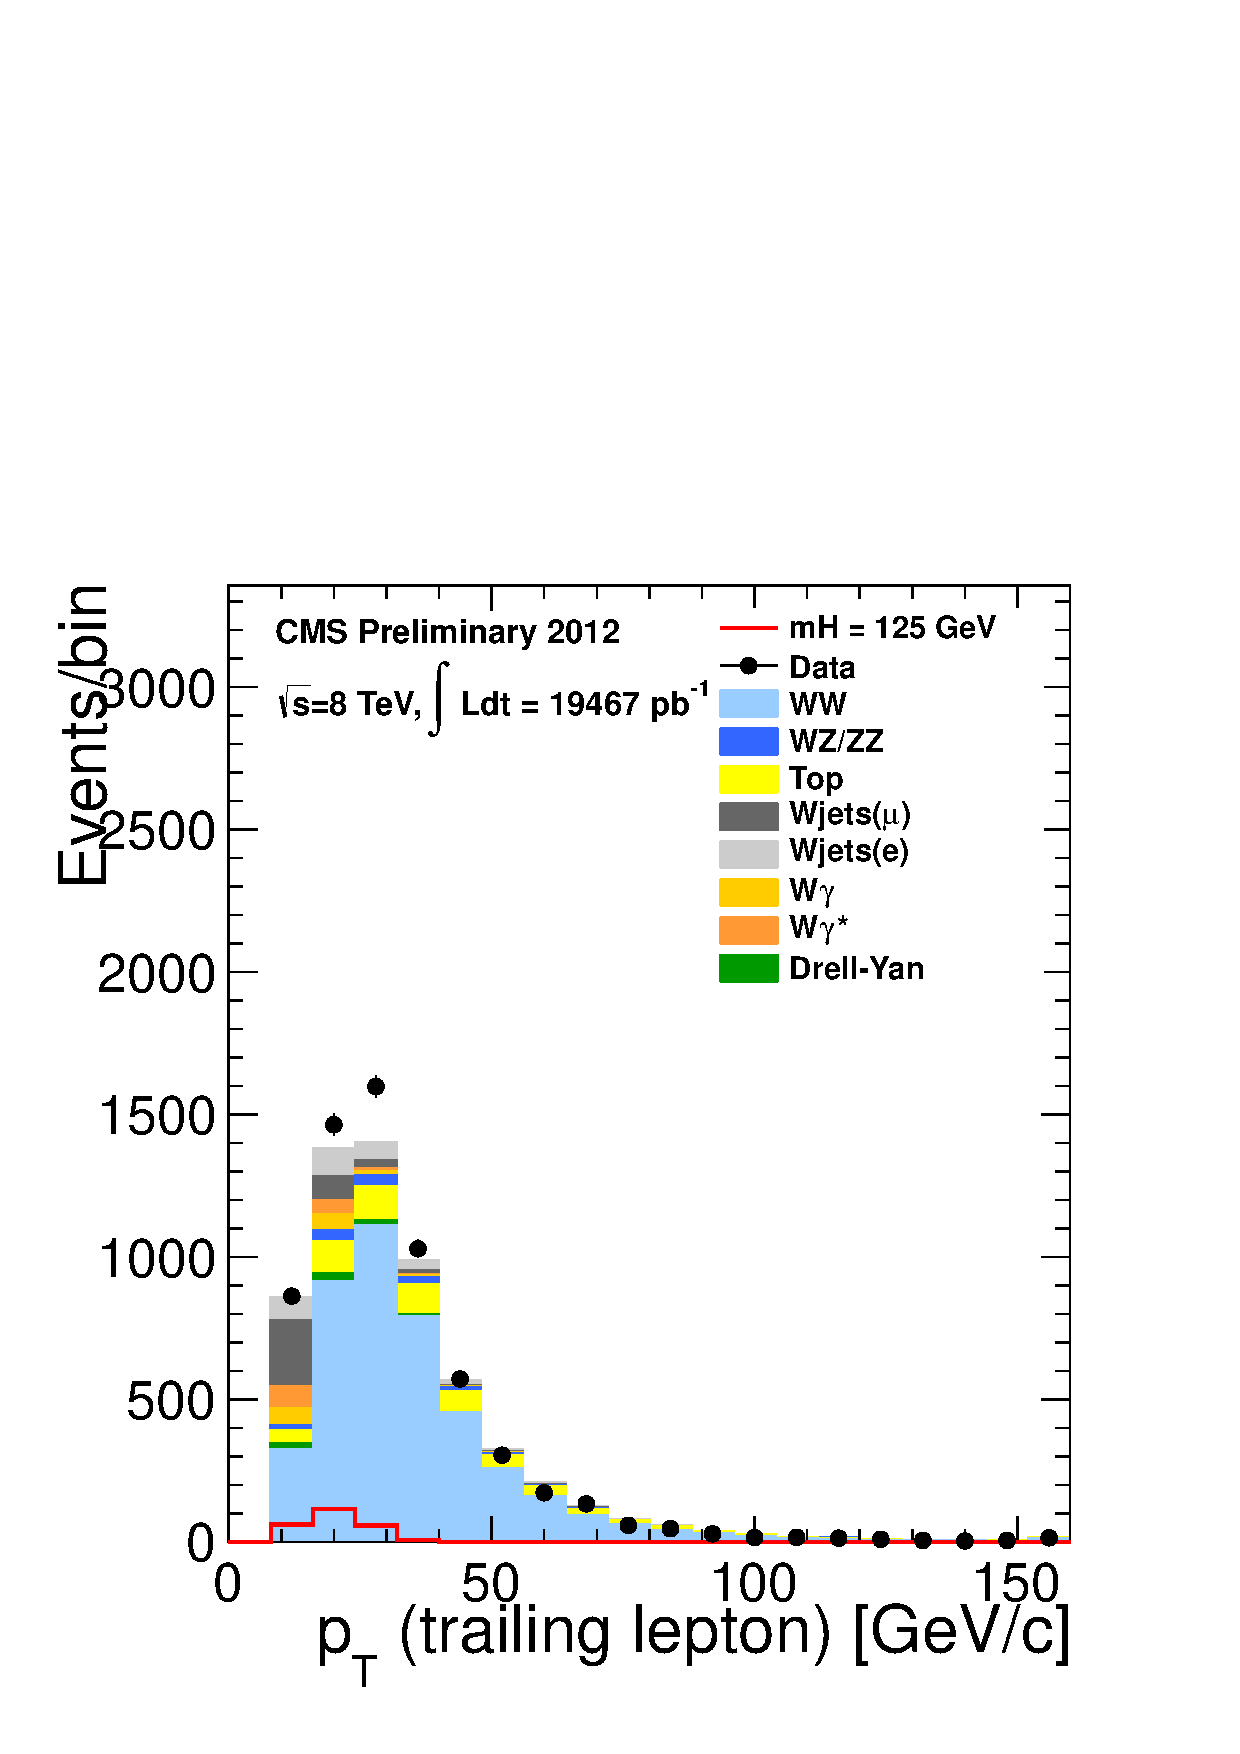
\includegraphics[width=.4\textwidth]{figures/hww_analysis16_0_ALL_of_0j_pt2.pdf}
}
\subfigure[1-Jet]{
\centering
\label{subfig:ww_ptmin_1j}
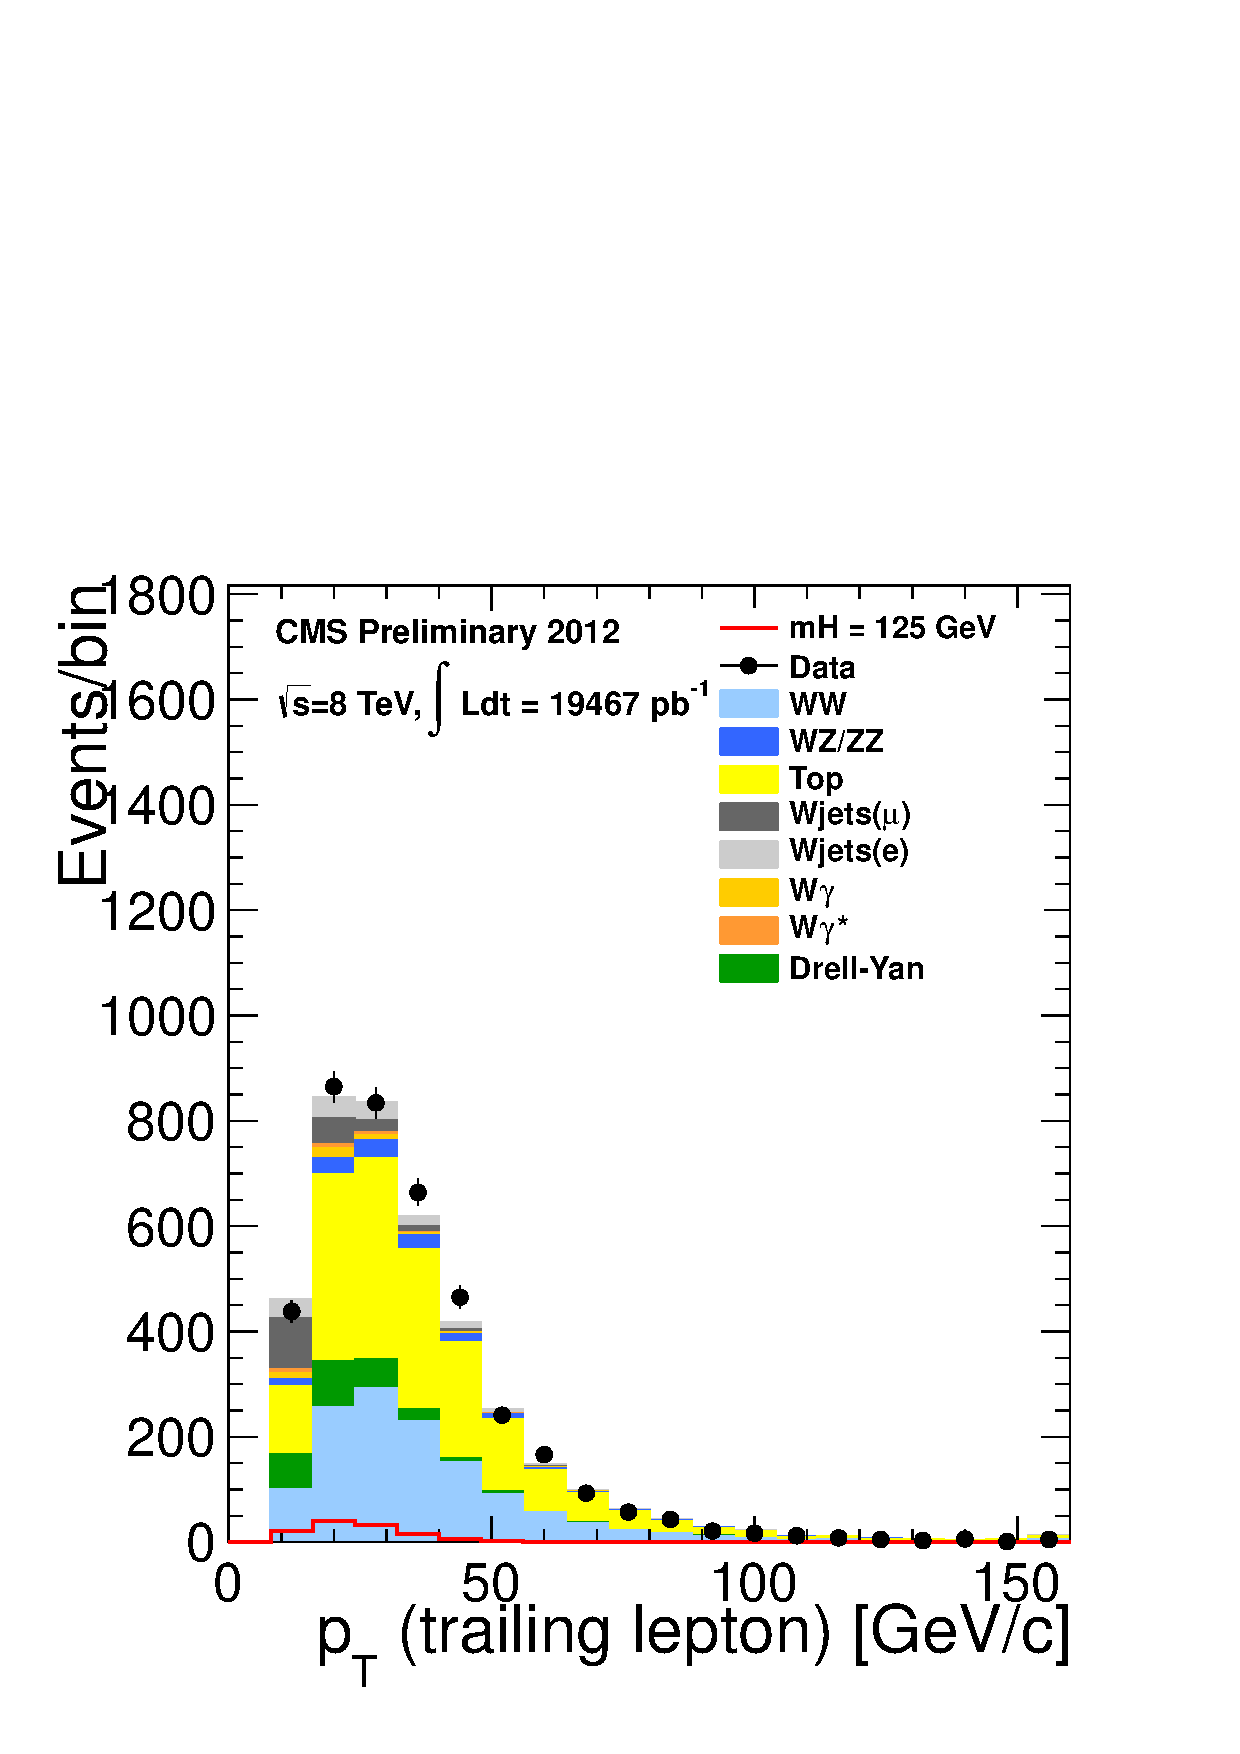
\includegraphics[width=.4\textwidth]{figures/hww_analysis16_0_ALL_of_1j_pt2.pdf}
}\\
\caption{Trailing lepton $p_T$ distribution after WW selection for \intlumiEightTeV of data 
of {\bf DF events} in 0-jet \subref{subfig:ww_ptmin_0j} 1-jet \subref{subfig:ww_ptmin_1j} bins. 
MC is scaled to data-driven estimates for all processes.} 
\label{fig:ww_ptmin}
\end{figure}

\begin{figure}[!hbtp]
\centering
\subfigure[0-Jet]{
\centering
\label{subfig:ww_ptmax_0j}
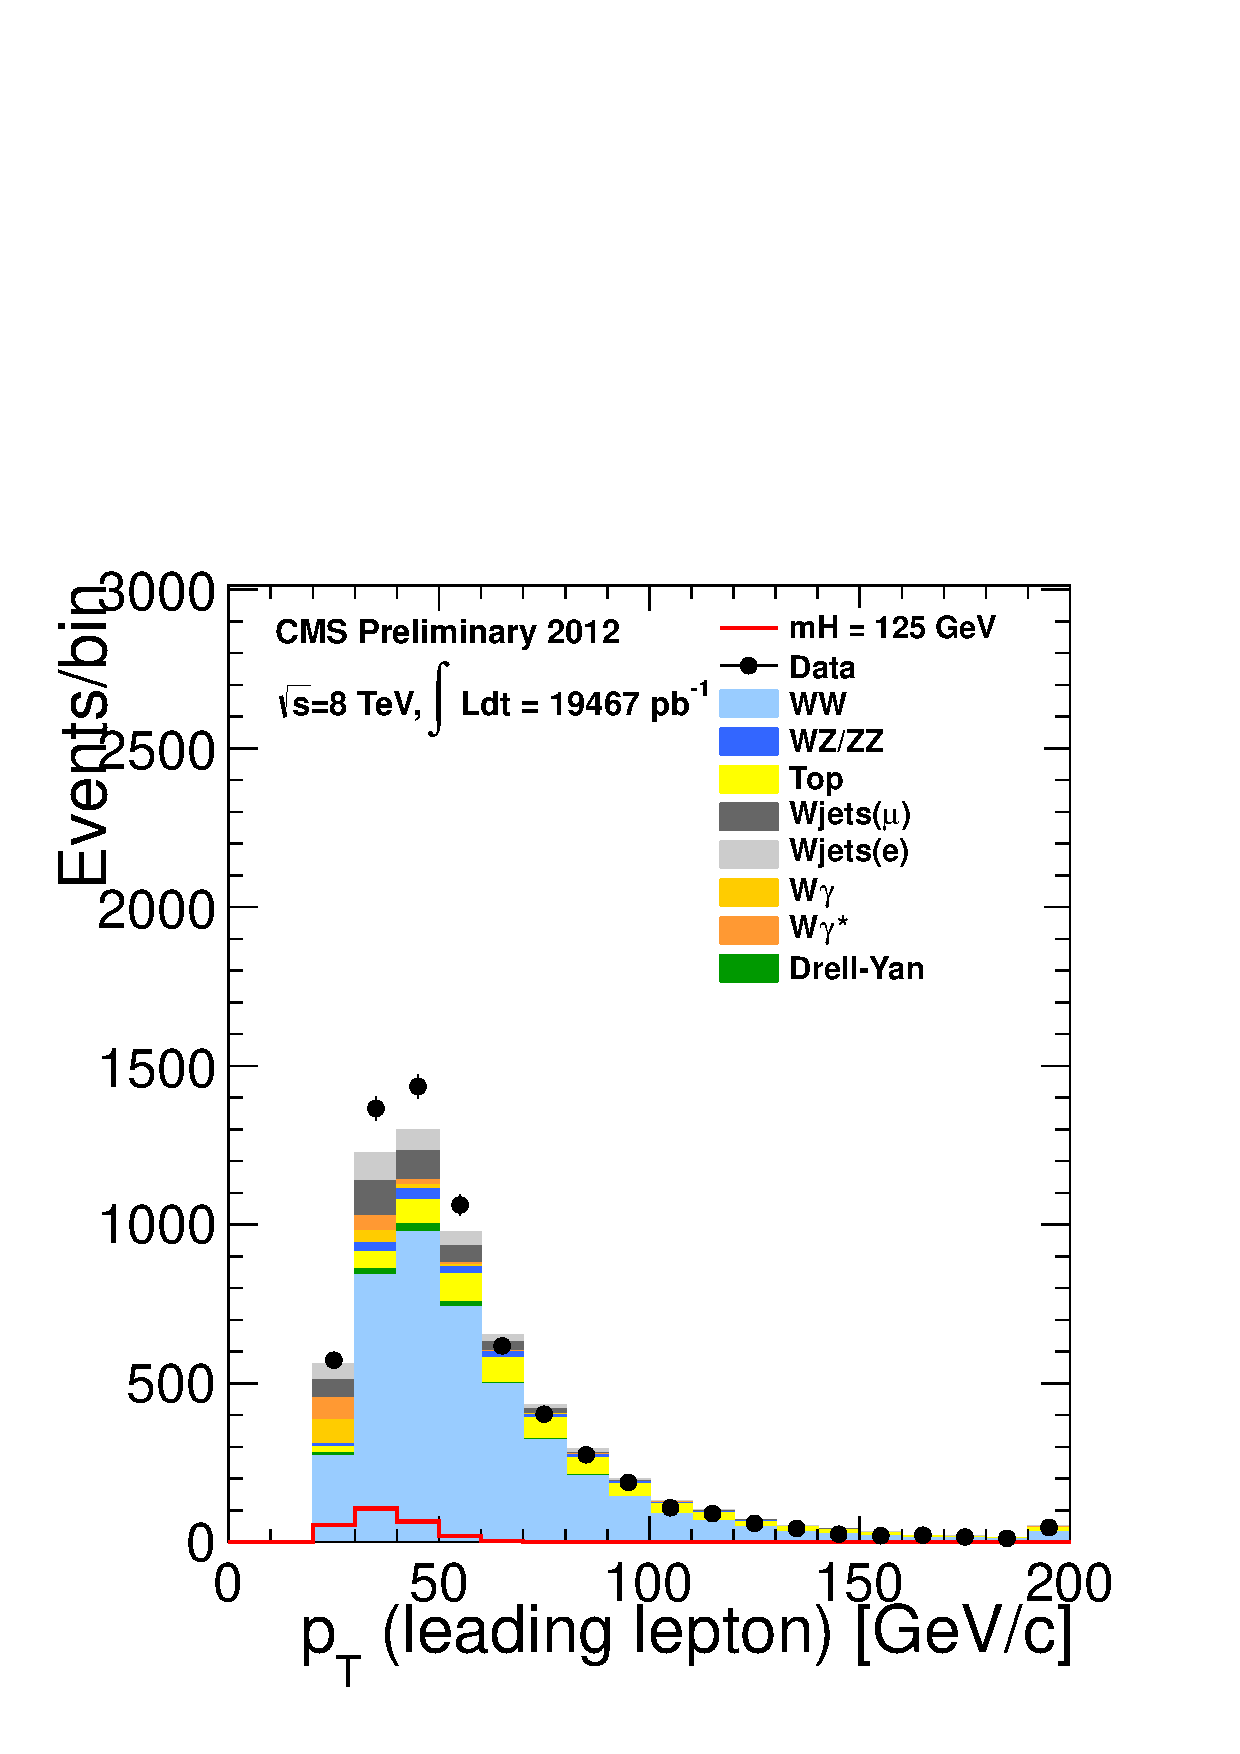
\includegraphics[width=.4\textwidth]{figures/hww_analysis16_0_ALL_of_0j_pt1.pdf}
}
\subfigure[1-Jet]{
\centering
\label{subfig:ww_ptmax_1j}
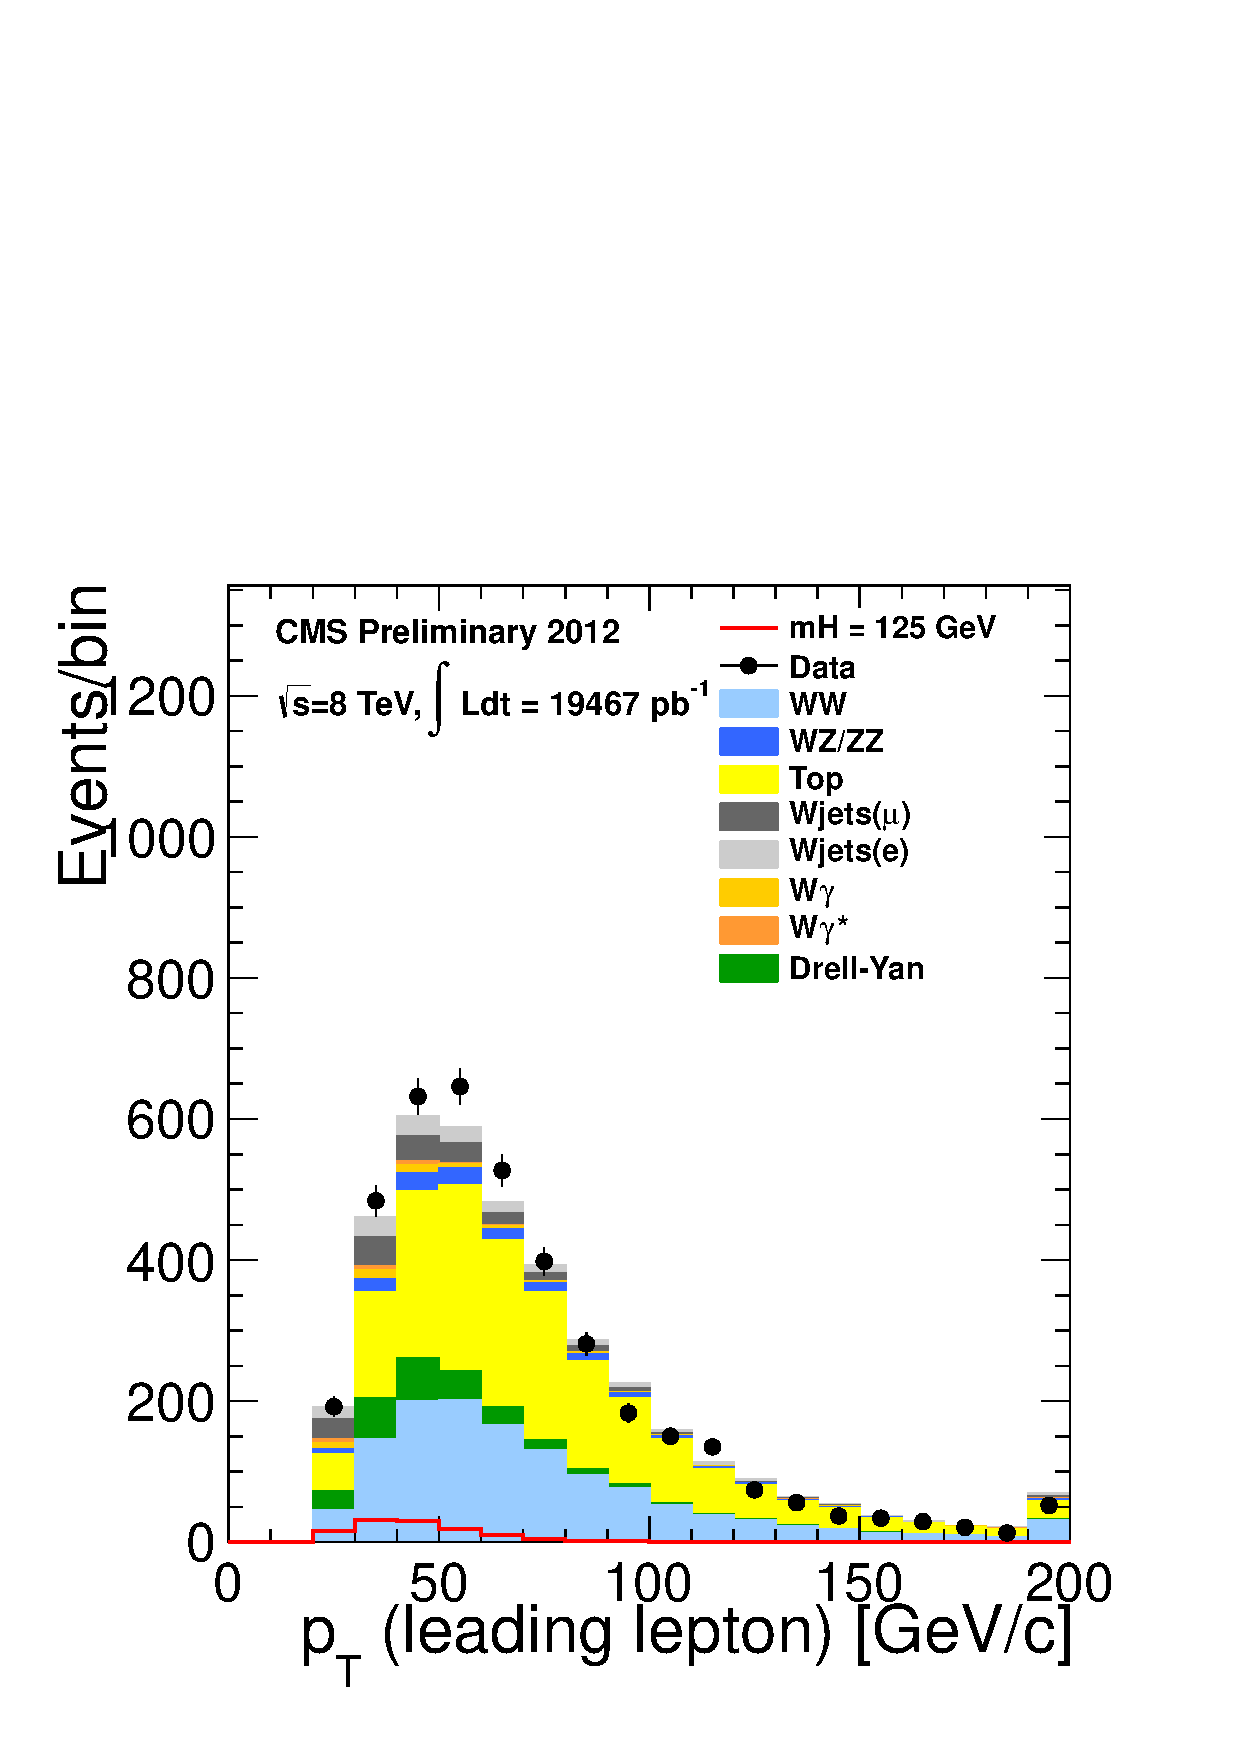
\includegraphics[width=.4\textwidth]{figures/hww_analysis16_0_ALL_of_1j_pt1.pdf}
}\\
\caption{Leading lepton $p_T$ distribution after WW selection for \intlumiEightTeV of data 
of {\bf DF events} in 0-jet \subref{subfig:ww_ptmax_0j} 1-jet \subref{subfig:ww_ptmax_1j} bins.  
MC is scaled to data-driven estimates for all processes.}
\label{fig:ww_ptmax}
\end{figure}

\begin{figure}[!hbtp]
\centering
\subfigure[0-Jet]{
\centering
\label{subfig:ww_pmet_0j}
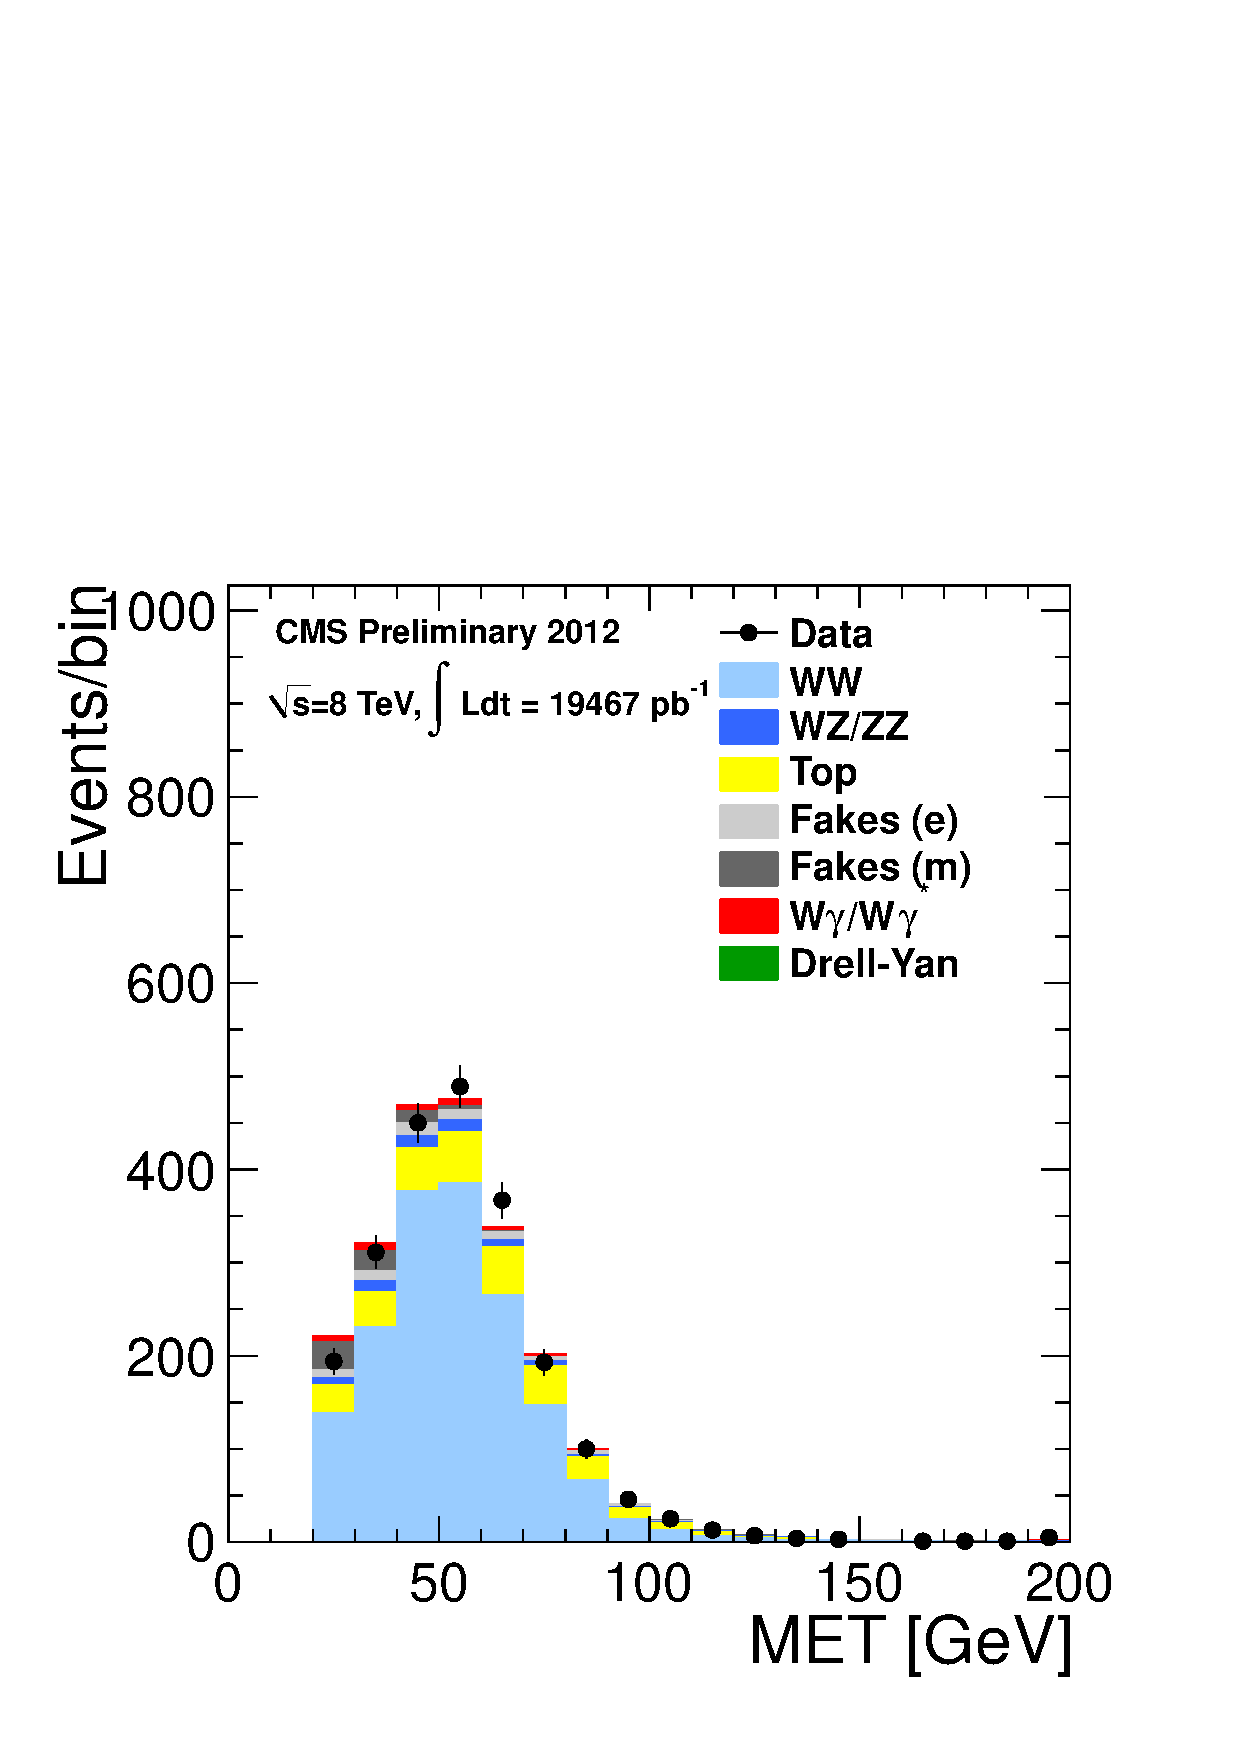
\includegraphics[width=.4\textwidth]{figures/hww_analysis16_0_ALL_of_0j_met.pdf}
}
\subfigure[1-Jet]{
\centering
\label{subfig:ww_pmet_1j}
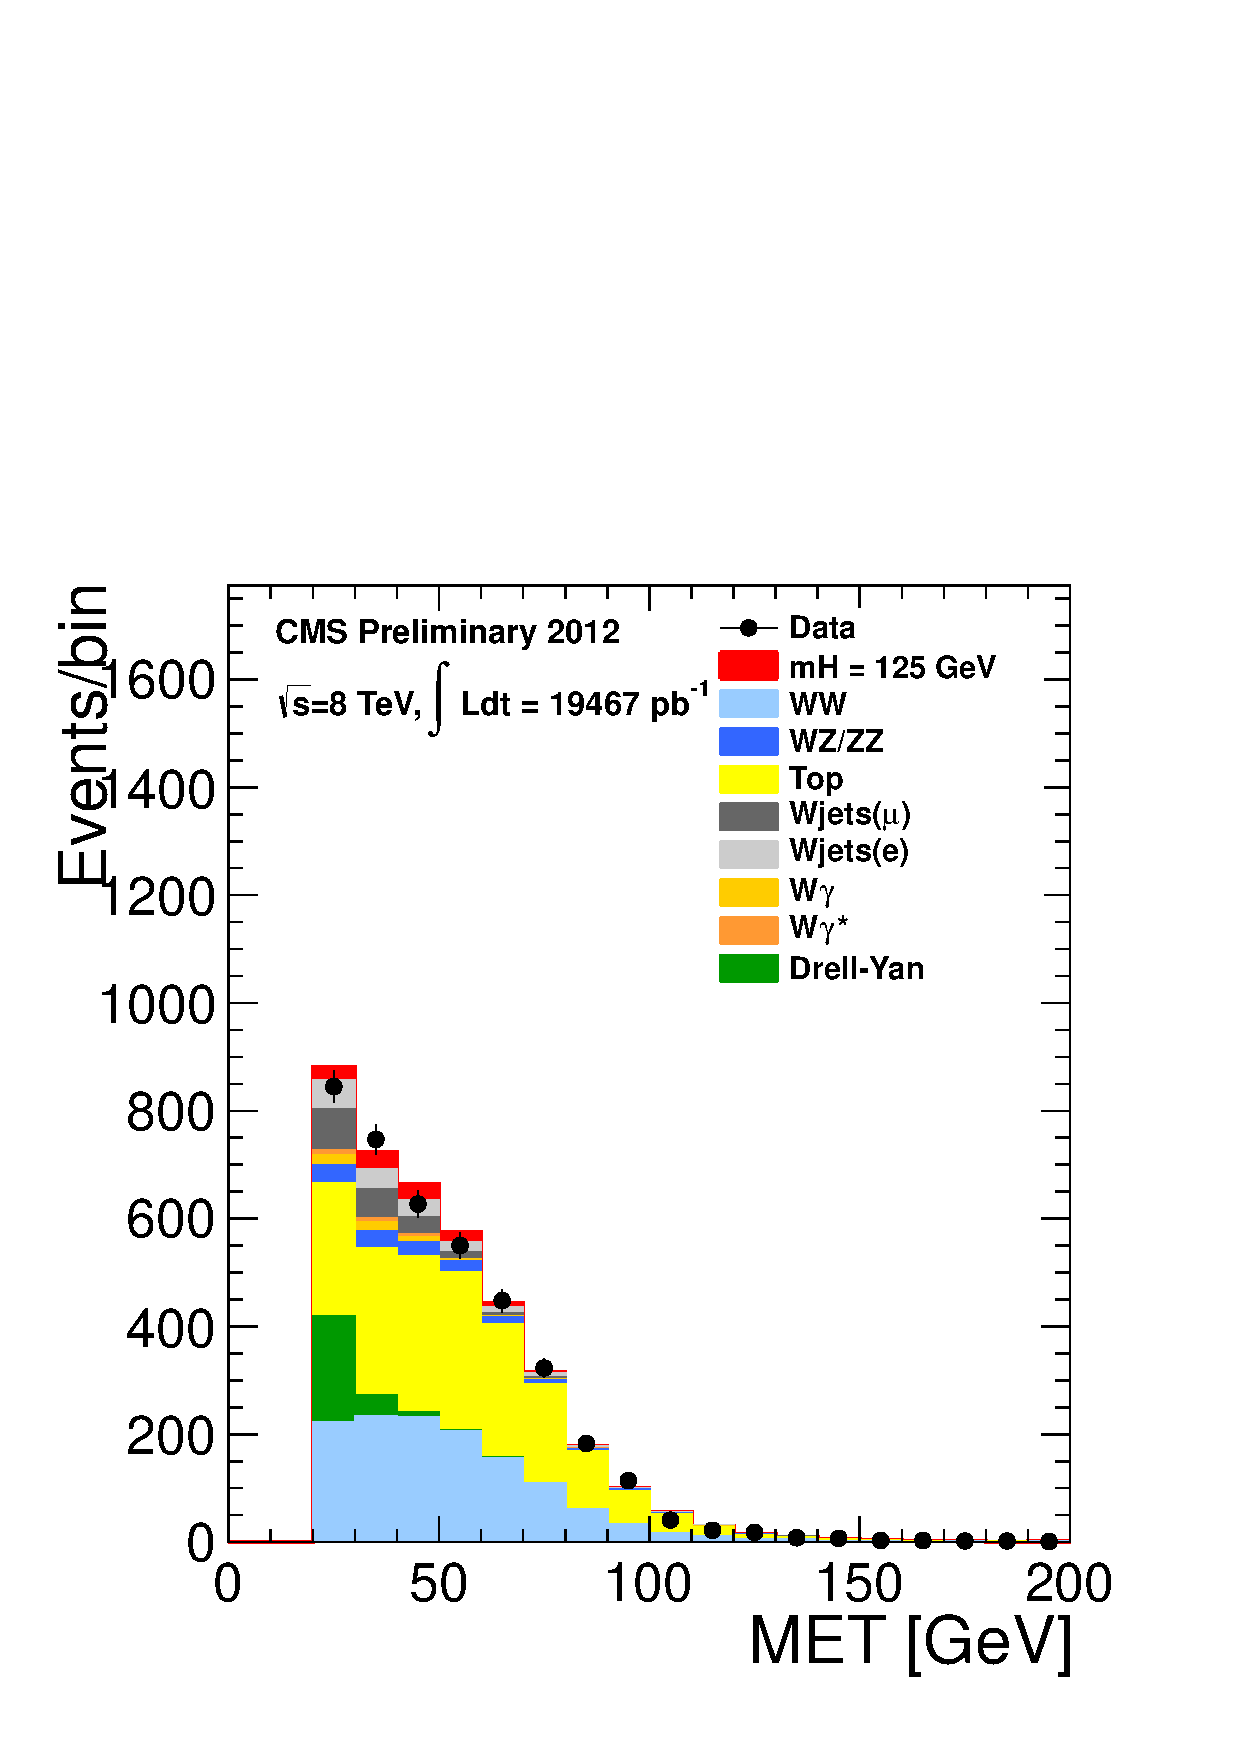
\includegraphics[width=.4\textwidth]{figures/hww_analysis16_0_ALL_of_1j_met.pdf}
}\\
\caption{The $\met$ distributions distribution after WW selection for \intlumiEightTeV of data 
of {\bf DF events} in 0-jet \subref{subfig:ww_pmet_0j} 1-jet \subref{subfig:ww_pmet_1j} bins.   
The MET variable plotted is $min(\text{proj}_\text{trk-MET}, \text{proj}_\text{PFMET})$. 
 MC is scaled to data-driven estimates for all processes.}
\label{fig:ww_pmet}
\end{figure}

\begin{figure}[!hbtp]
\centering
\subfigure[0-Jet]{
\centering
\label{subfig:ww_mt_0j}
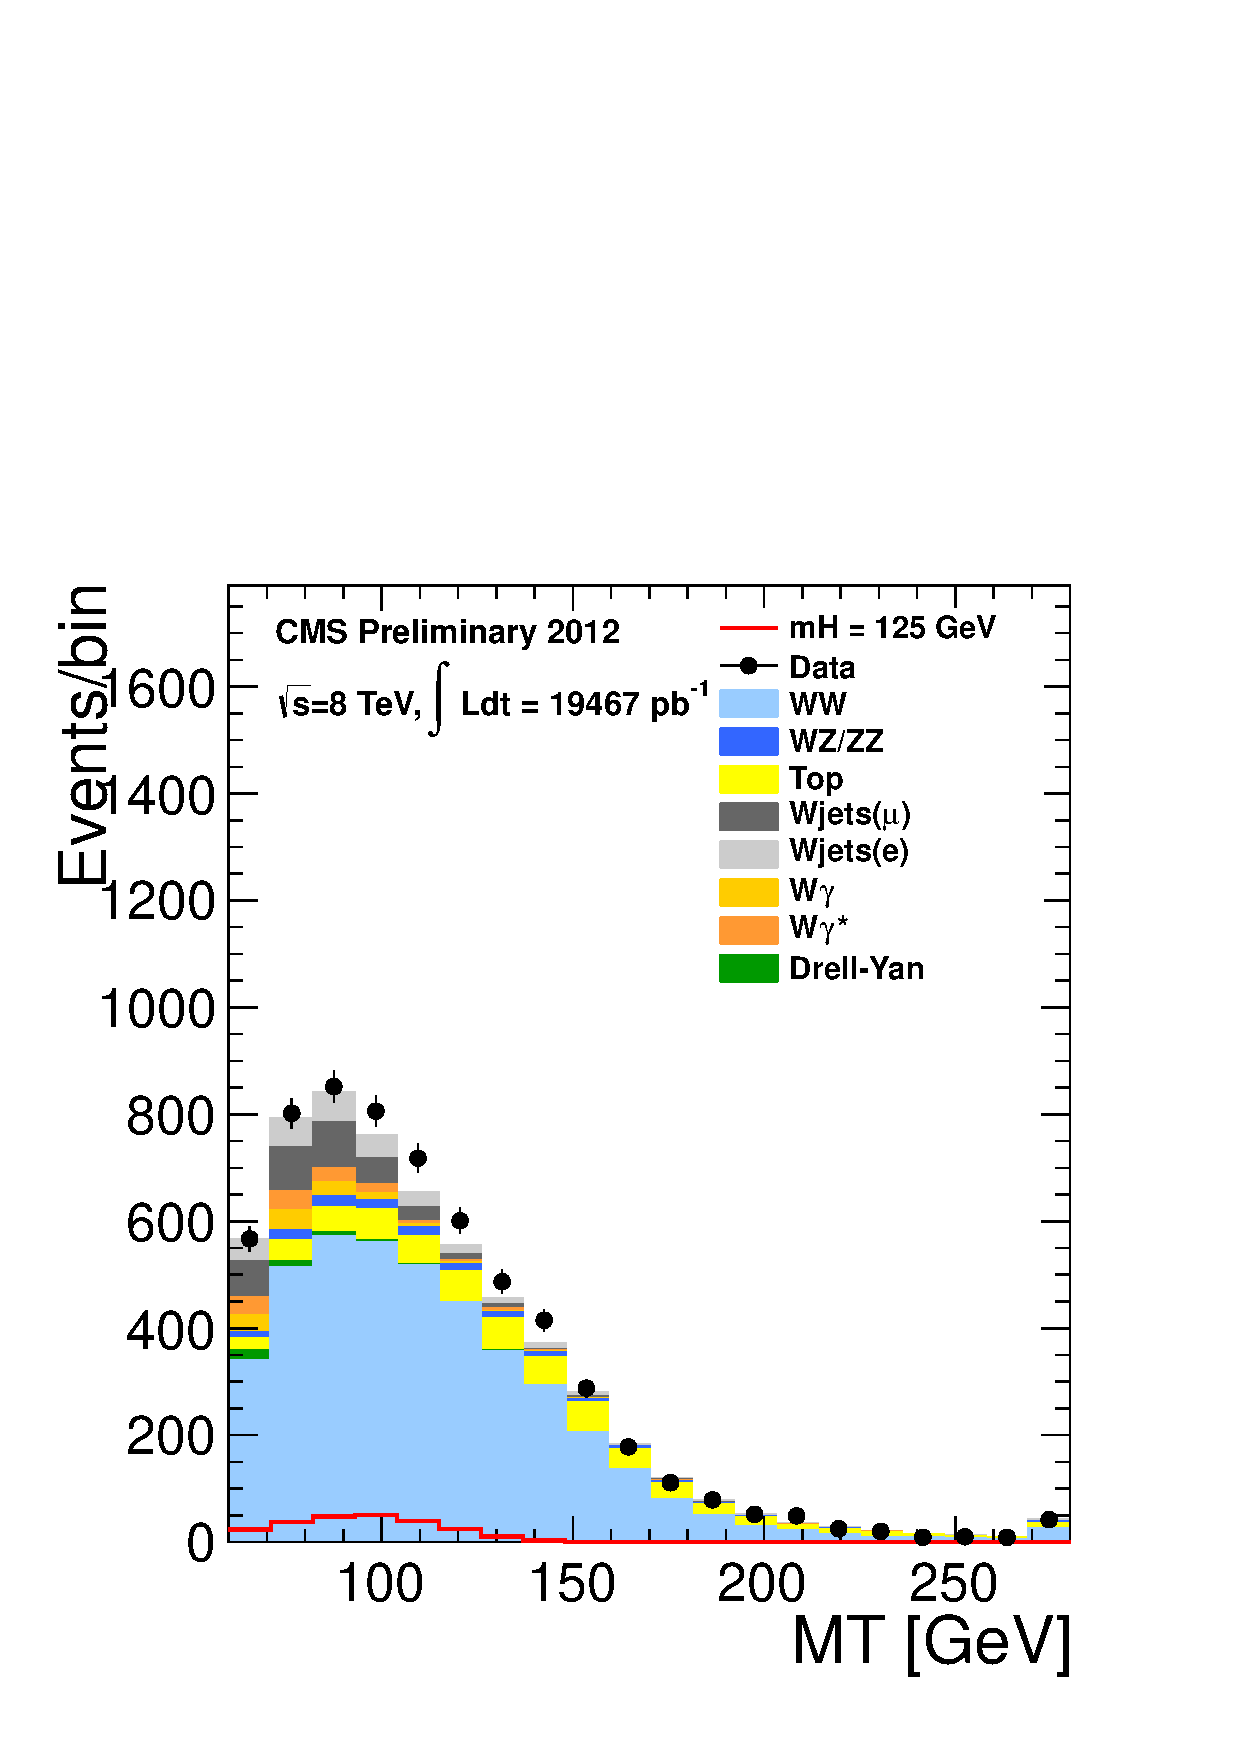
\includegraphics[width=.4\textwidth]{figures/hww_analysis16_0_ALL_of_0j_mt.pdf}
}
\subfigure[1-Jet]{
\centering
\label{subfig:ww_mt_1j}
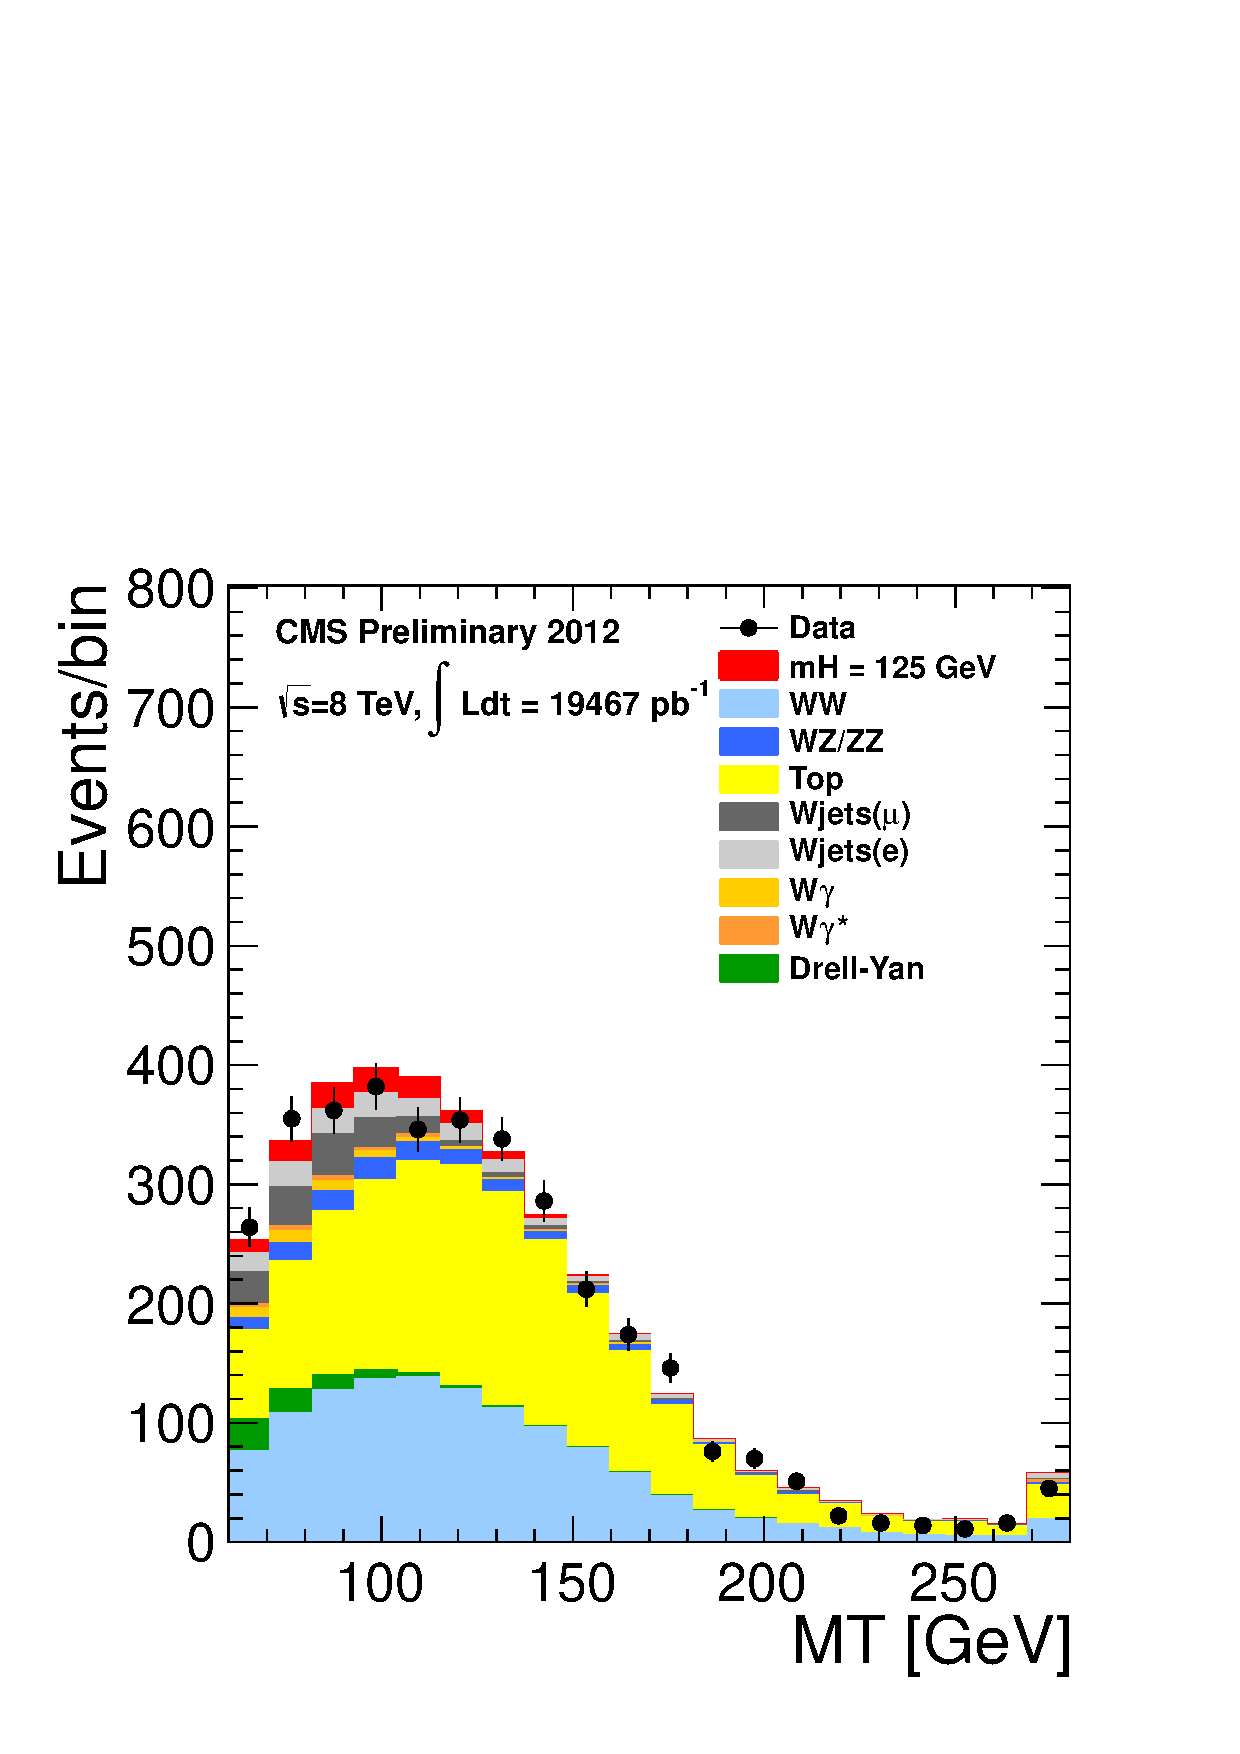
\includegraphics[width=.4\textwidth]{figures/hww_analysis16_0_ALL_of_1j_mt.pdf}
} \\
\caption{Transverse mass distribution after WW selection for \intlumiEightTeV of data 
of {\bf DF events} in 0-jet \subref{subfig:ww_mt_0j} 1-jet \subref{subfig:ww_mt_1j} bins.   
MC is scaled to data-driven estimates for all processes.}
\label{fig:ww_mt}
\end{figure}

\begin{figure}[!hbtp]
\centering
\subfigure[0-Jet]{
\centering
\label{subfig:ww_dilmass_0j}
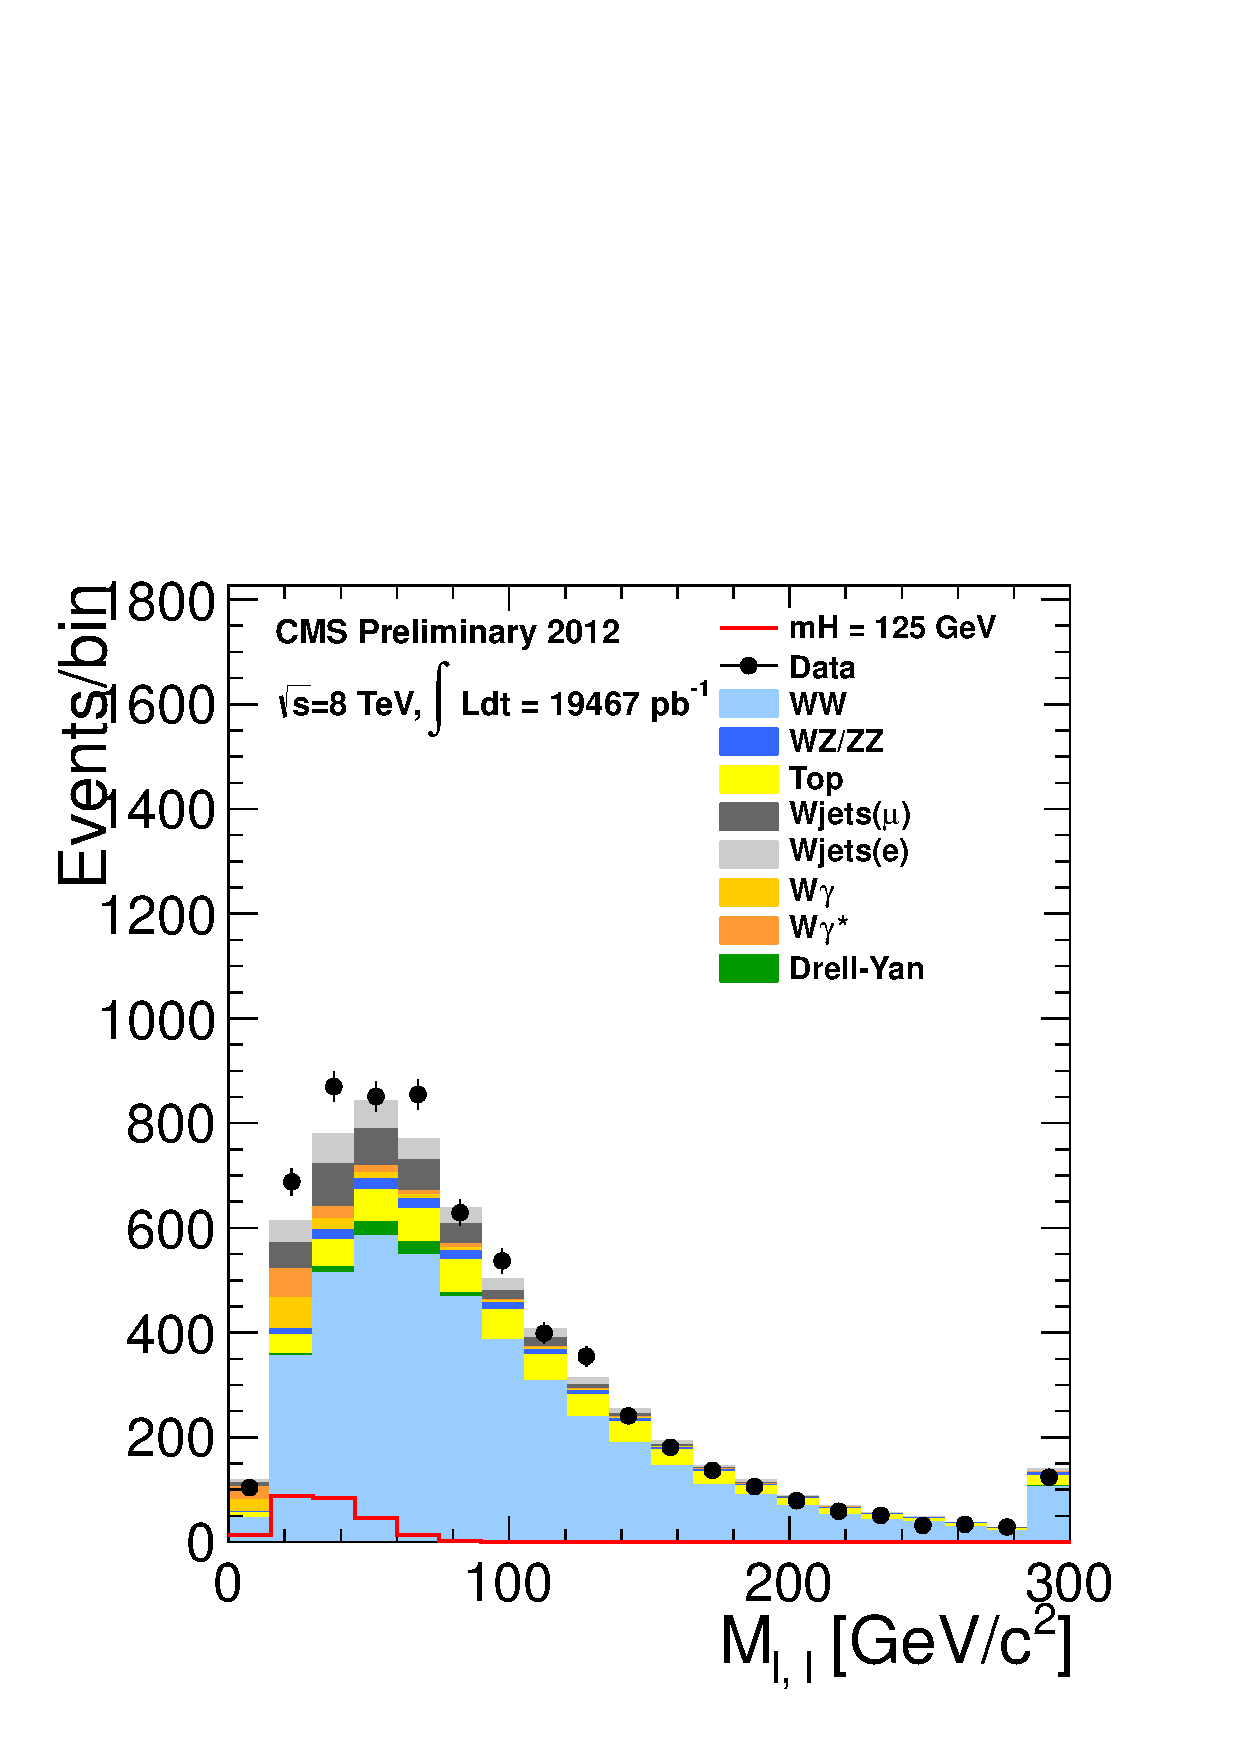
\includegraphics[width=.4\textwidth]{figures/hww_analysis16_0_ALL_of_0j_mll.pdf}
}
\subfigure[1-Jet]{
\centering
\label{subfig:ww_dilmass_1j}
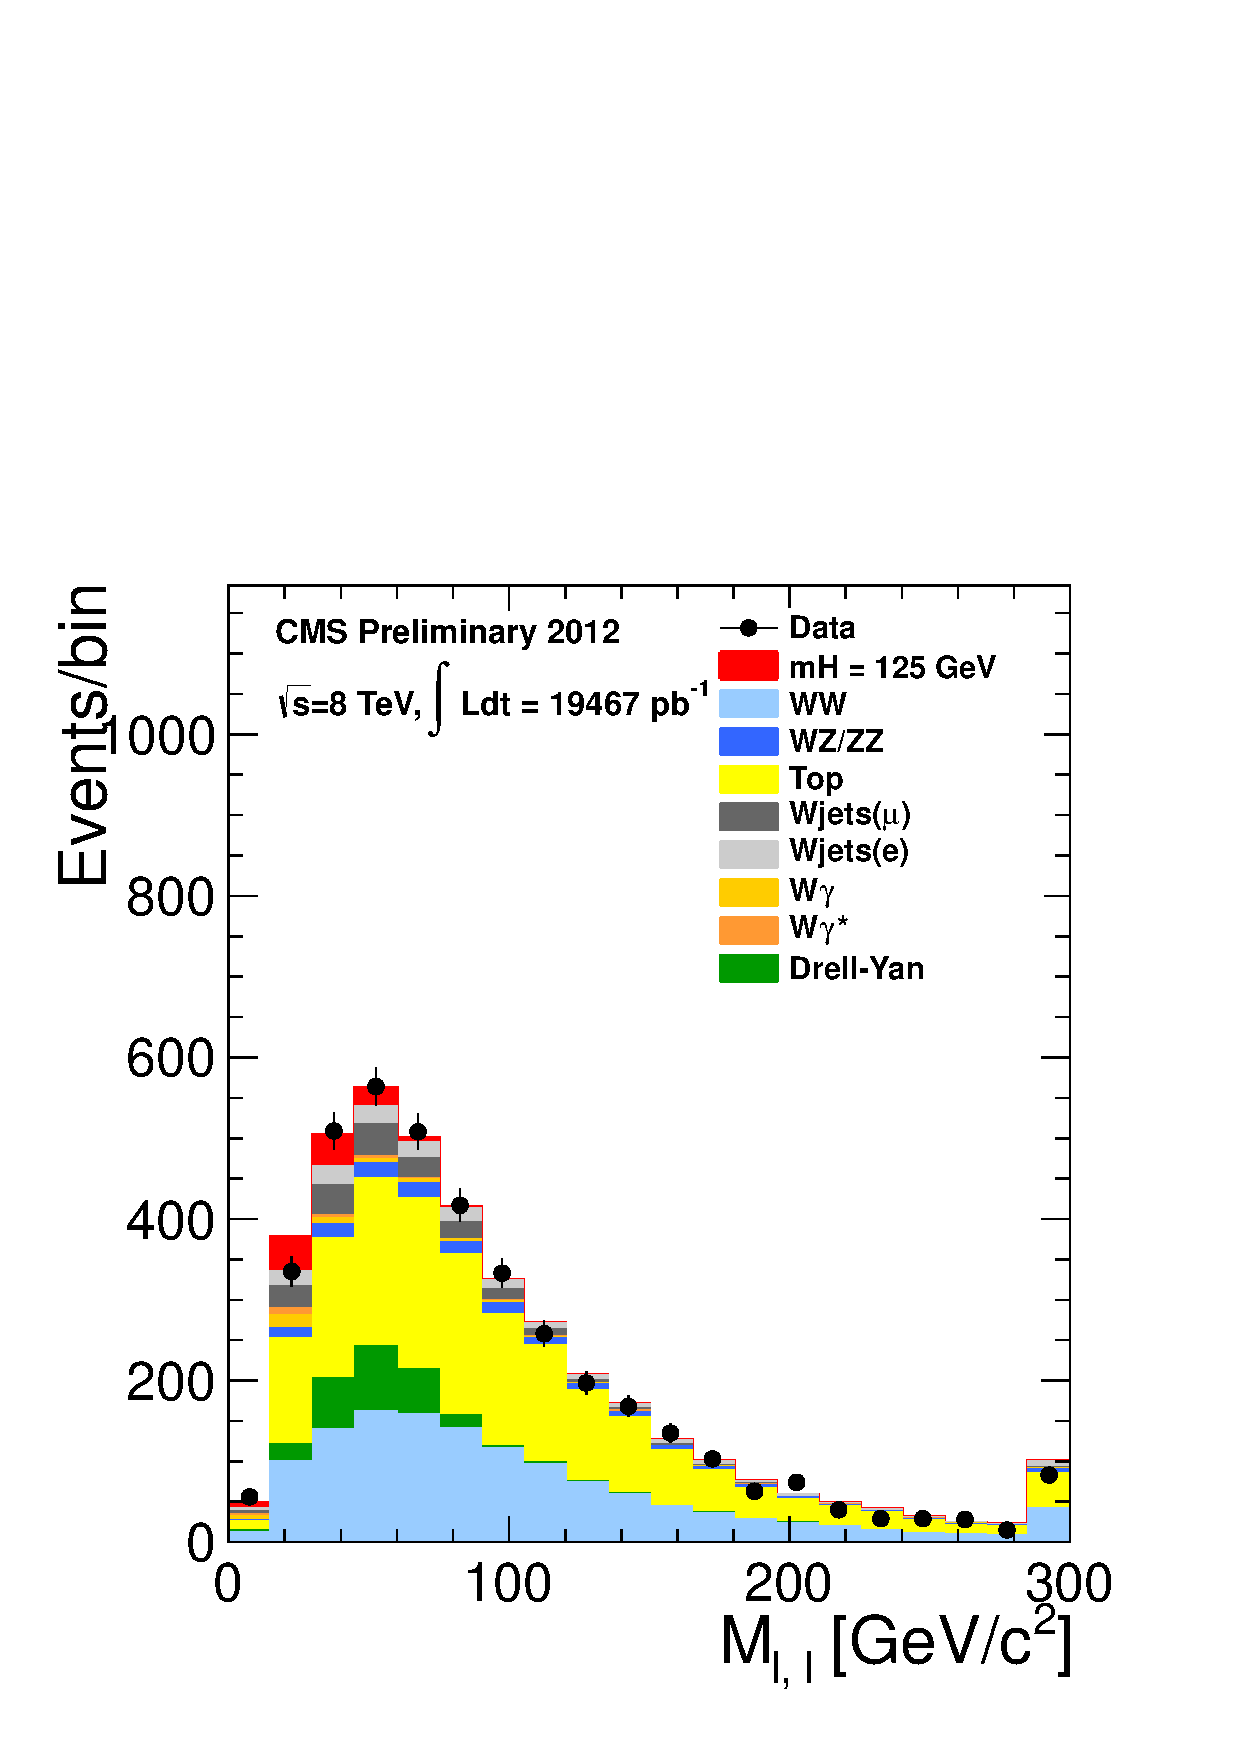
\includegraphics[width=.4\textwidth]{figures/hww_analysis16_0_ALL_of_1j_mll.pdf}
} \\
\caption{Invariant dilepton mass distribution after WW selection for \intlumiEightTeV of data  
of {\bf DF events} in 0-jet \subref{subfig:ww_dilmass_0j} 1-jet \subref{subfig:ww_dilmass_1j} bins.   
MC is scaled to data-driven estimates for all processes.}
\label{fig:ww_dilmass}
\end{figure}

\begin{figure}[!hbtp]
\centering
\subfigure[0-Jet]{
\centering
\label{subfig:ww_deltaphi_0j}
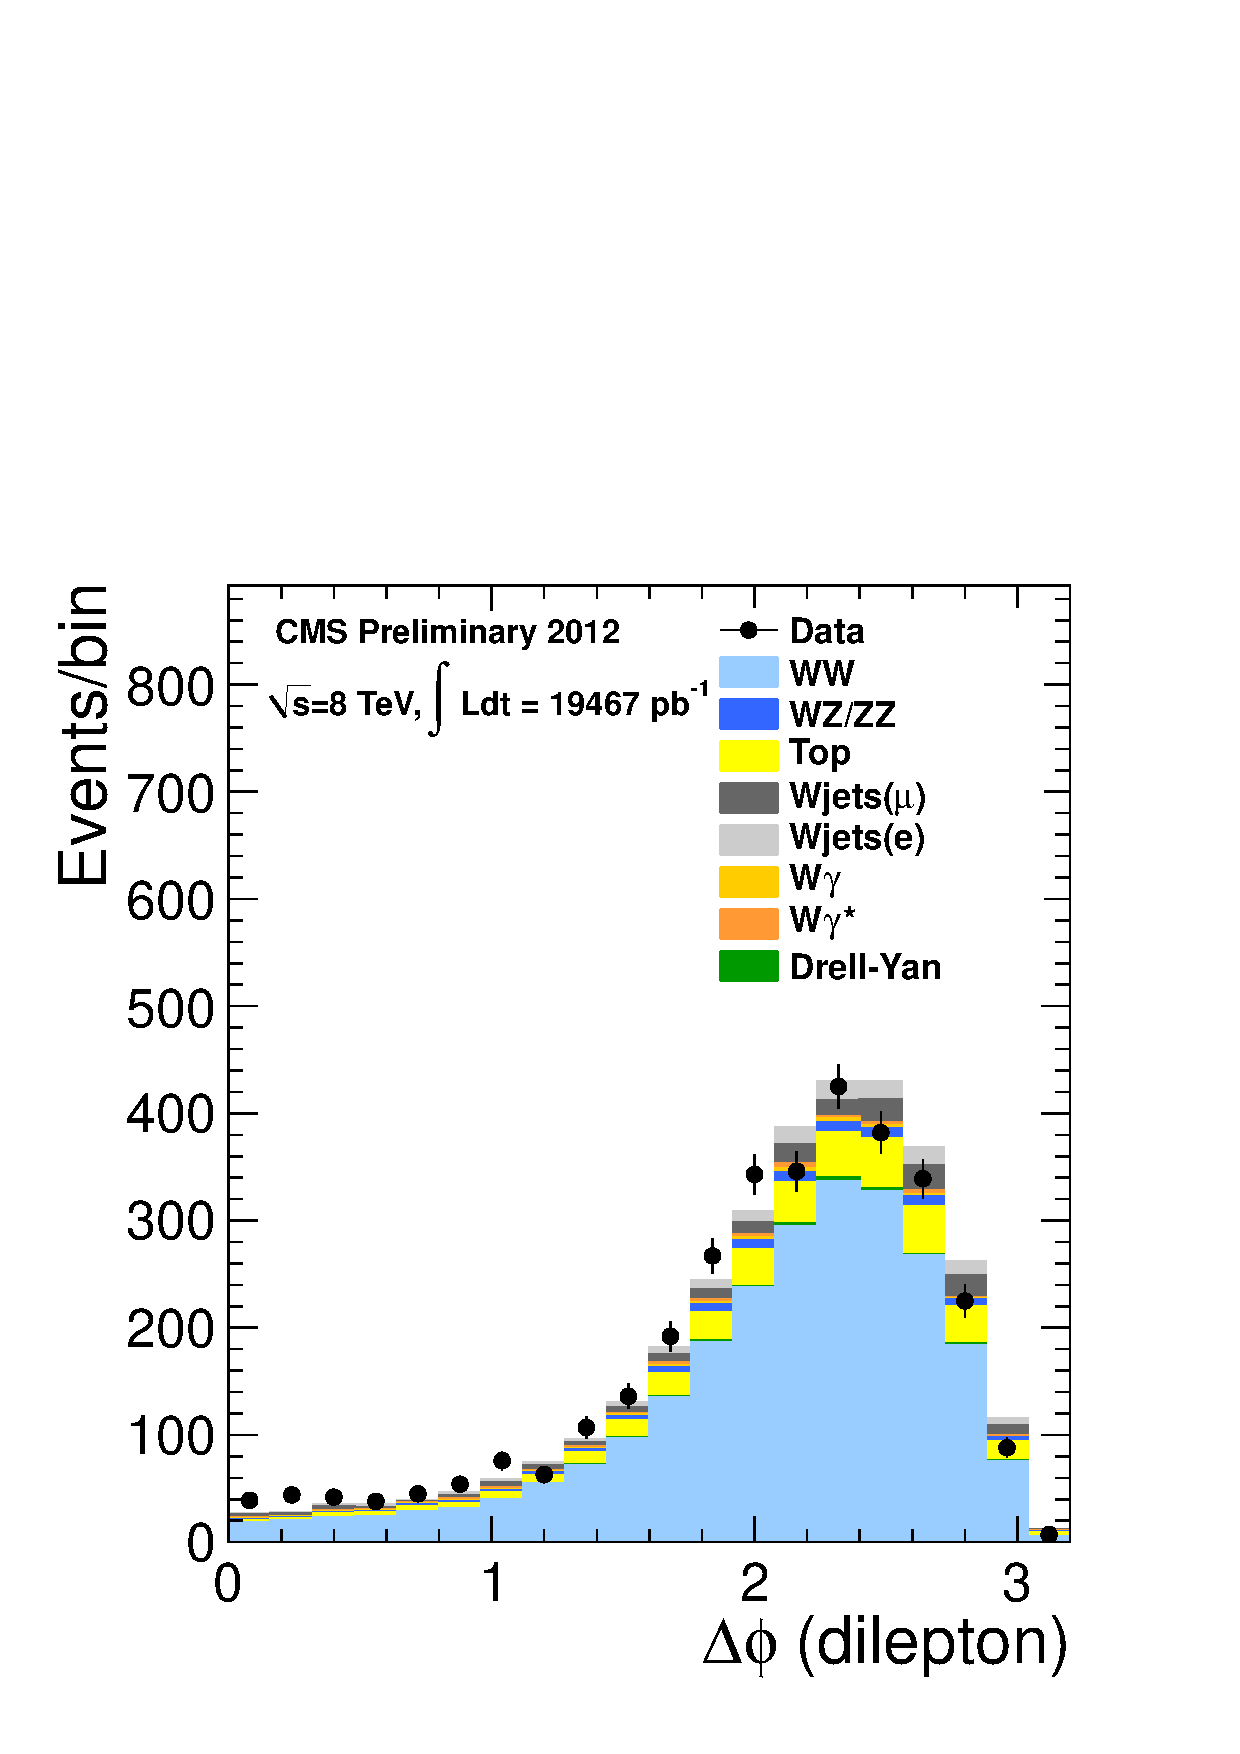
\includegraphics[width=.4\textwidth]{figures/hww_analysis16_0_ALL_of_0j_dphi.pdf}
}
\subfigure[1-Jet]{
\centering
\label{subfig:ww_deltaphi_1j}
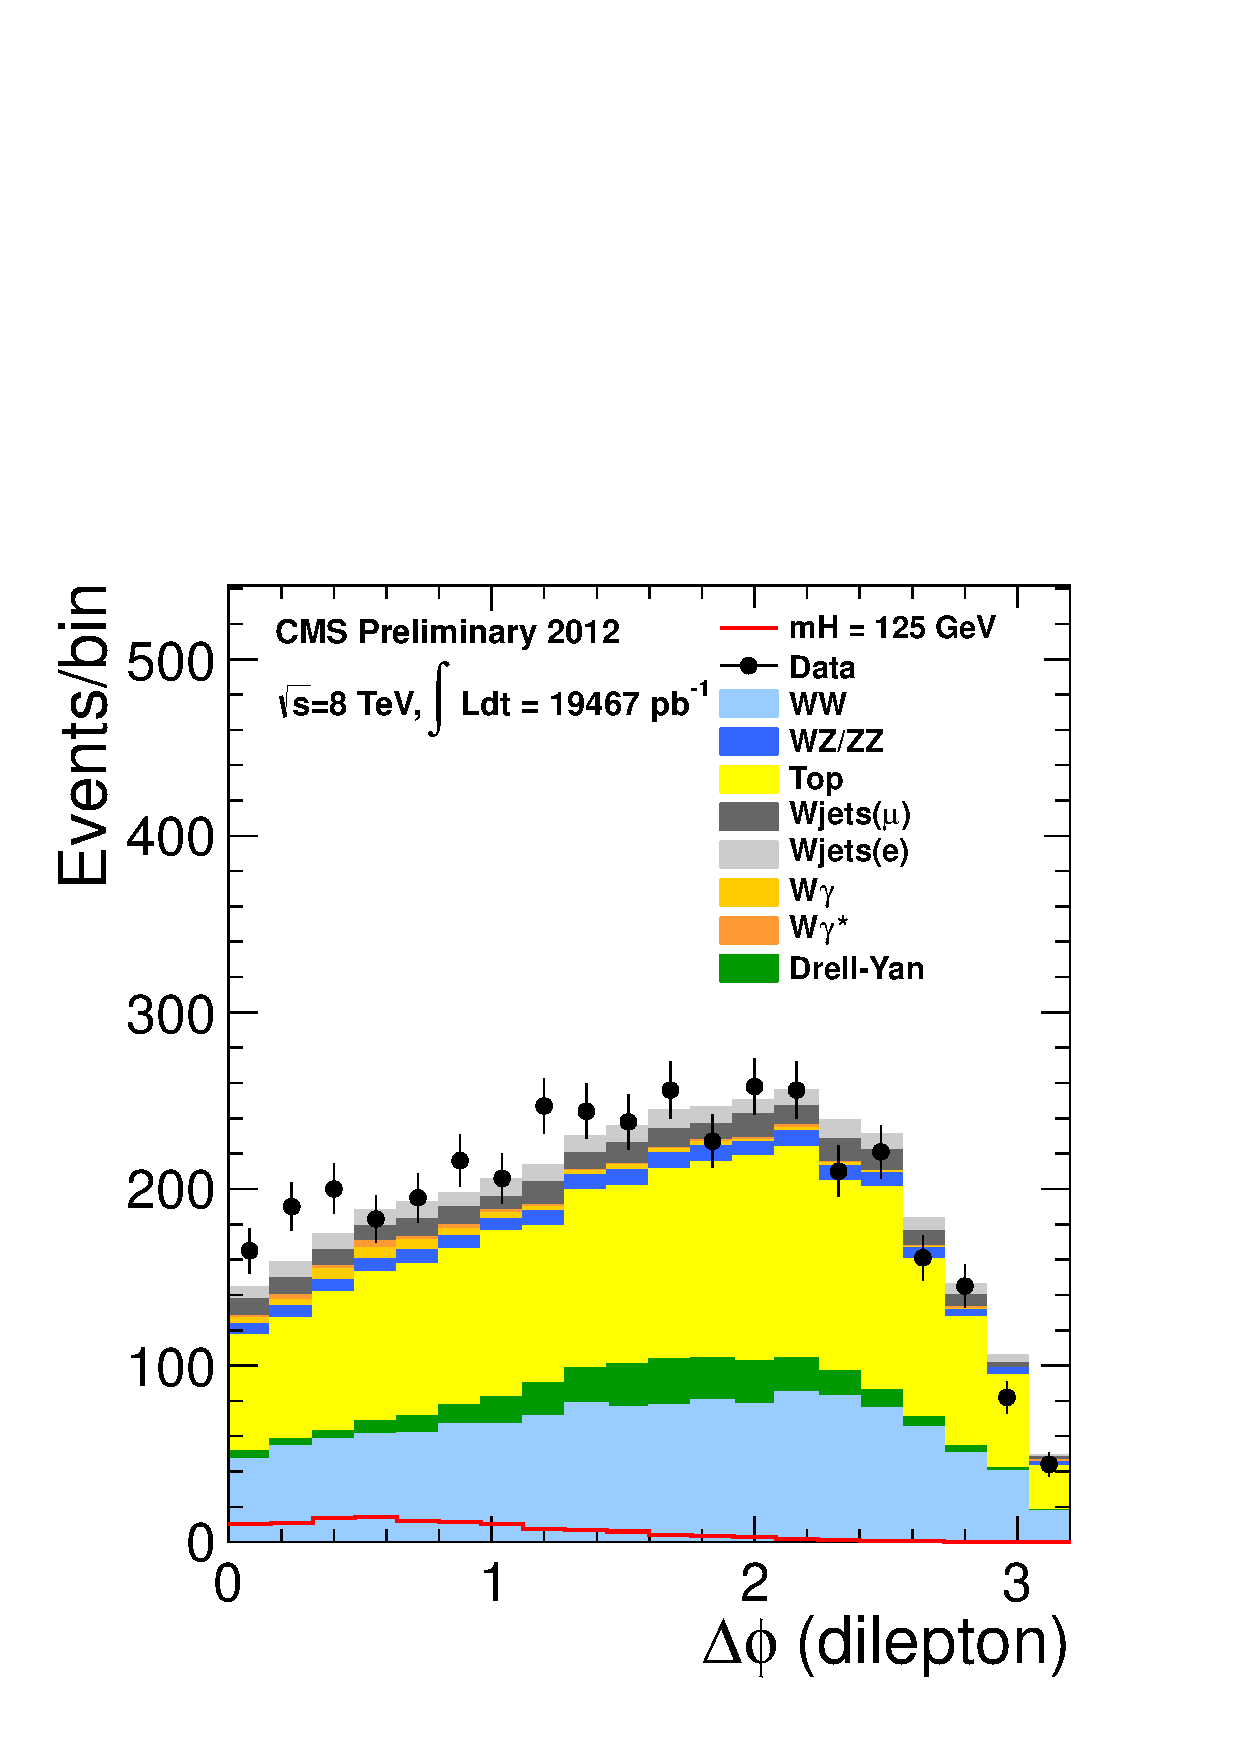
\includegraphics[width=.4\textwidth]{figures/hww_analysis16_0_ALL_of_1j_dphi.pdf}
} \\
\caption{Dilepton $\Delta\phi$ distribution after WW selection for \intlumiEightTeV of data 
of {\bf DF events} in 0-jet \subref{subfig:ww_deltaphi_0j} 1-jet \subref{subfig:ww_deltaphi_1j} bins.   
MC is scaled to data-driven estimates.}
\label{fig:ww_deltaphi}
\end{figure}

%%%%%%%%%%%%%%%%%%%%%%%%%%%%%%%%%%%%%%%%%%%%%%%%%%%%%%%%%%% 
\begin{table}[ht!]
\begin{center}
\begin{tabular}{c | c | c } 
\hline
            & \multicolumn{1}{c|}{0-jet} & \multicolumn{1}{c}{1-jet} \\
mass [\GeV] & scale factor & scale factor \\
\hline
            \multicolumn{3}{c}{Cut-based} \\
\hline
 115 &  1.10  $\pm$  0.06  &  0.93  $\pm$  0.10 \\
 120 &  1.10  $\pm$  0.06  &  0.93  $\pm$  0.10 \\
 125 &  1.10  $\pm$  0.06  &  0.93  $\pm$  0.10 \\
 130 &  1.10  $\pm$  0.06  &  0.93  $\pm$  0.10 \\
 135 &  1.10  $\pm$  0.06  &  0.93  $\pm$  0.09 \\
 140 &  1.10  $\pm$  0.06  &  0.93  $\pm$  0.09 \\
 150 &  1.08  $\pm$  0.06  &  0.93  $\pm$  0.10 \\
 160 &  1.08  $\pm$  0.06  &  0.93  $\pm$  0.10 \\
 170 &  1.07  $\pm$  0.06  &  0.92  $\pm$  0.10 \\
 180 &  1.07  $\pm$  0.06  &  0.92  $\pm$  0.10 \\
 190 &  1.07  $\pm$  0.06  &  0.92  $\pm$  0.10 \\
 200 &  1.07  $\pm$  0.06  &  0.91  $\pm$  0.10 \\
\hline \hline
            \multicolumn{3}{c}{Shape} \\
\hline
All masses & 1.19  $\pm$  0.06  &  1.09  $\pm$  0.10 \\
\hline
\end{tabular}
\caption{WW background estimation for cut-based and shape analyses.}
\label{tab:ww_est}
\end{center}
\end{table}

%%%%%%%%%%%%%%%%%%%%%%%%%%%%%%
%%%%%%%%%%%%%%%%%%%%%%%%%%%%%%
\clearpage
\subsection{Final Results for the Higgs Search with \intlumiEightTeV{}}
\label{sec:search_results_8tev}

The observed and expected upper limits at 95\% C.L. using 2D analysis in DF 0/1 jet categories 
and cut-based analysis in SF 0/1 jet categories 
are shown in Table~\ref{tab:uls_8tev} and Figure \ref{fig:uls_8tev}.
The observed and expected upper limits at 95\% C.L. using cut-based analysis in DF/SF 0/1 jet categories 
are shown in Table~\ref{tab:uls_cut_8tev} and Figure \ref{fig:uls_cut_8tev}.
The observed and expected significances are shown in Table~\ref{tab:significance_8tev}. 

%%%%%%%%%%%%%%%%%
% plot
\begin{figure}[!hbtp]
\centering
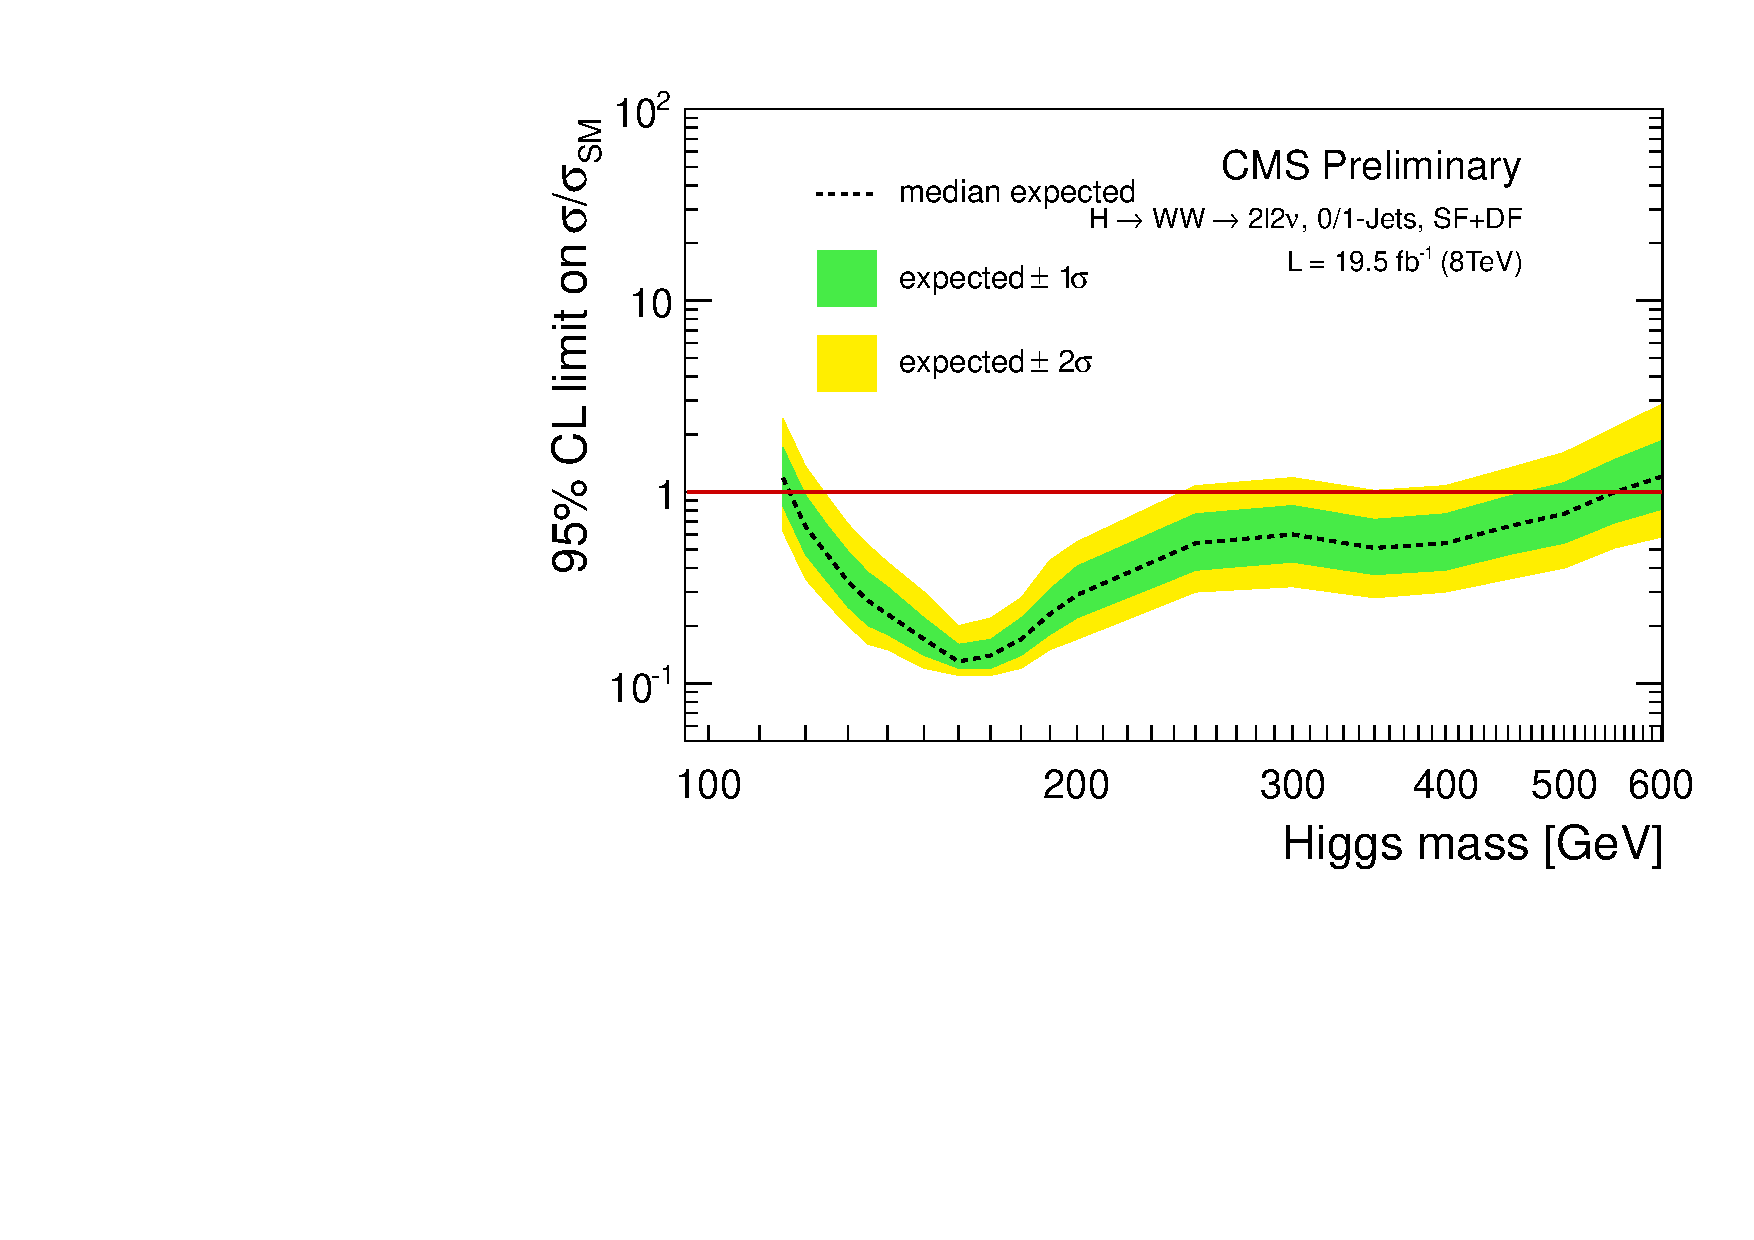
\includegraphics[width=.75\textwidth]{figures/table_limits_nj_8TeV_log.pdf}
\caption{Observed and expected upper limits for SM Higgs in $\intlumiEightTeV$ at 8 TeV in 0/1jet final state. 
2D(cut-based) analysis is used in the DF(SF) final states.}  
\label{fig:uls_8tev}
\end{figure}
% table
\begin{table}[!htbp]
\begin{center}
\begin{tabular}{c c c c c}
\hline
\vspace{-3mm} && \\
Higgs Mass & Observed  & Median expected & Expected range for 68\% & Expected range for 95\%   \\
\hline
110 & 5.07 & 2.17 & [1.54, 3.14] & [1.14, 4.44] \\
115 & 2.71 & 1.10 & [0.78, 1.59] & [0.58, 2.26] \\
120 & 1.64 & 0.67 & [0.48, 0.97] & [0.36, 1.38] \\
125 & 1.23 & 0.44 & [0.32, 0.63] & [0.24, 0.89] \\
130 & 0.87 & 0.32 & [0.24, 0.46] & [0.19, 0.64] \\
135 & 0.72 & 0.26 & [0.19, 0.36] & [0.16, 0.50] \\
140 & 0.61 & 0.22 & [0.17, 0.30] & [0.14, 0.41] \\
150 & 0.39 & 0.17 & [0.14, 0.22] & [0.12, 0.30] \\
160 & 0.23 & 0.13 & [0.12, 0.16] & [0.11, 0.20] \\
170 & 0.23 & 0.14 & [0.12, 0.17] & [0.11, 0.22] \\
180 & 0.32 & 0.17 & [0.14, 0.22] & [0.12, 0.29] \\
190 & 0.46 & 0.23 & [0.18, 0.32] & [0.15, 0.43] \\
200 & 0.45 & 0.30 & [0.22, 0.41] & [0.18, 0.57] \\
250 & 0.46 & 0.51 & [0.36, 0.72] & [0.28, 1.01] \\
300 & 0.46 & 0.55 & [0.40, 0.78] & [0.30, 1.10] \\
350 & 0.32 & 0.46 & [0.33, 0.66] & [0.26, 0.93] \\
400 & 0.31 & 0.49 & [0.35, 0.70] & [0.27, 0.97] \\
450 & 0.36 & 0.59 & [0.42, 0.85] & [0.32, 1.20] \\
500 & 0.52 & 0.78 & [0.55, 1.13] & [0.41, 1.63] \\
550 & 0.72 & 1.00 & [0.69, 1.48] & [0.51, 2.18] \\
600 & 1.08 & 1.19 & [0.80, 1.84] & [0.58, 2.84] \\
\vspace{-3mm} && \\
\hline
\end{tabular}
\caption{Observed and expected upper limits for SM Higgs in $\intlumiEightTeV$ at 8 TeV in 0/1jet final state. 
2D(cut-based) analysis is used in the DF(SF) final states.}  
\label{tab:uls_8tev}
\end{center}
\end{table}
%%%%%%%%%%


%%%%%%%%%%%%%%%%%
% plot
\begin{figure}[!hbtp]
\centering
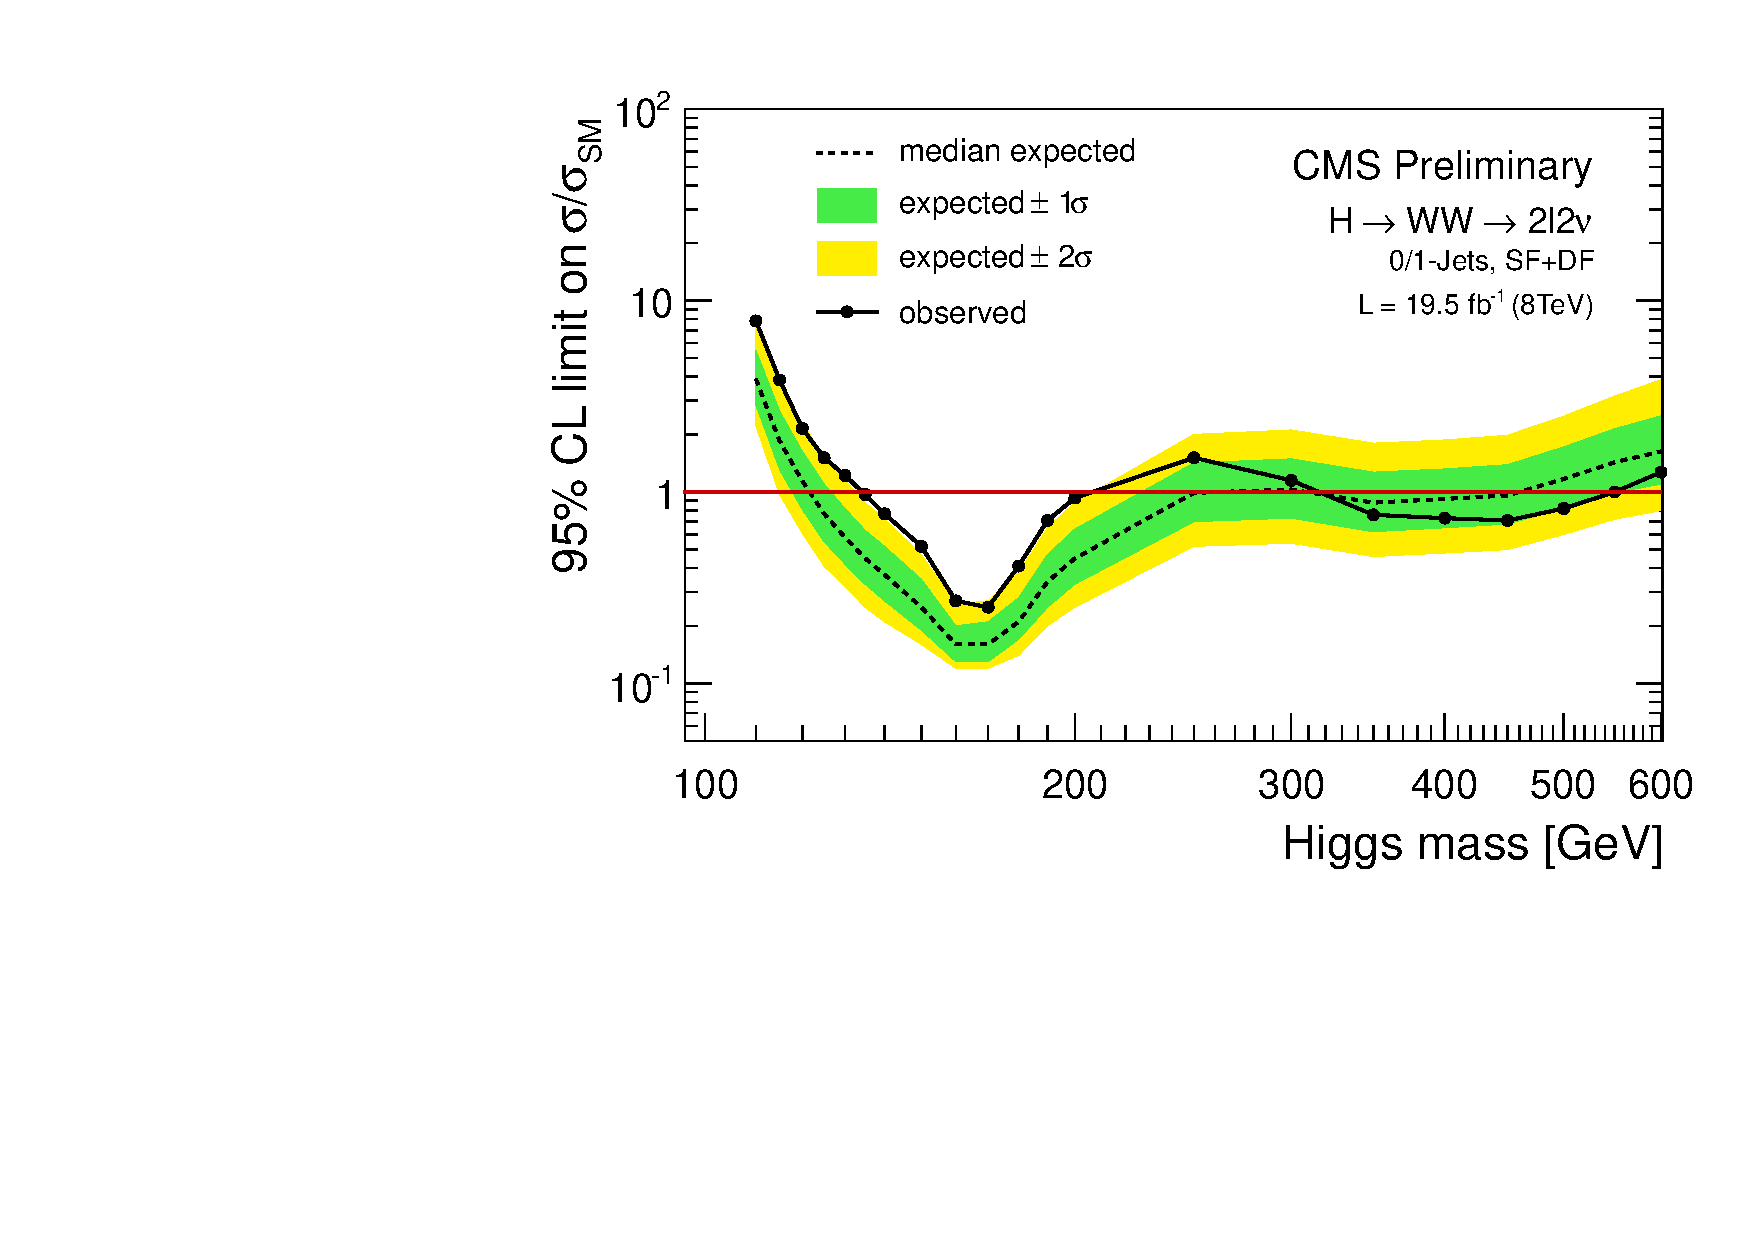
\includegraphics[width=.75\textwidth]{figures/table_limits_nj_cut_8TeV_log.pdf}
\caption{Observed and expected upper limits for SM Higgs in $\intlumiEightTeV$ at 8 TeV in 0/1jet final state. 
Cut-based analysis is used in the DF/SF final states.}  
\label{fig:uls_cut_8tev}
\end{figure}
% table
\begin{table}[!htbp]
\begin{center}
\begin{tabular}{c c c c c}
\hline
\vspace{-3mm} && \\
Higgs Mass & Observed  & Median expected & Expected range for 68\% & Expected range for 95\%   \\
\hline
110 & 7.83 & 3.90 & [2.85, 5.51] & [2.21, 7.68] \\
115 & 3.85 & 1.85 & [1.31, 2.65] & [0.97, 3.72] \\
120 & 2.15 & 1.14 & [0.81, 1.63] & [0.61, 2.29] \\
125 & 1.51 & 0.77 & [0.55, 1.10] & [0.41, 1.53] \\
130 & 1.22 & 0.58 & [0.42, 0.82] & [0.32, 1.15] \\
135 & 0.97 & 0.45 & [0.33, 0.63] & [0.25, 0.88] \\
140 & 0.77 & 0.37 & [0.27, 0.52] & [0.21, 0.72] \\
150 & 0.52 & 0.25 & [0.19, 0.35] & [0.16, 0.47] \\
160 & 0.27 & 0.16 & [0.13, 0.20] & [0.12, 0.26] \\
170 & 0.25 & 0.16 & [0.13, 0.21] & [0.12, 0.27] \\
180 & 0.41 & 0.21 & [0.17, 0.28] & [0.14, 0.38] \\
190 & 0.71 & 0.34 & [0.25, 0.47] & [0.20, 0.65] \\
200 & 0.93 & 0.45 & [0.33, 0.64] & [0.25, 0.88] \\
250 & 1.51 & 0.99 & [0.70, 1.42] & [0.52, 2.00] \\
300 & 1.15 & 1.03 & [0.73, 1.49] & [0.54, 2.11] \\
350 & 0.76 & 0.88 & [0.62, 1.27] & [0.46, 1.80] \\
400 & 0.73 & 0.92 & [0.65, 1.32] & [0.48, 1.87] \\
450 & 0.71 & 0.96 & [0.68, 1.39] & [0.50, 1.98] \\
500 & 0.82 & 1.17 & [0.82, 1.72] & [0.60, 2.49] \\
550 & 1.00 & 1.43 & [0.99, 2.14] & [0.72, 3.17] \\
600 & 1.27 & 1.63 & [1.10, 2.50] & [0.80, 3.86] \\
\vspace{-3mm} && \\
\hline
\end{tabular}
\caption{Observed and expected upper limits for SM Higgs in $\intlumiEightTeV$ at 8 TeV in 0/1jet final state. 
Cut-based analysis is used in the DF/SF final states.}  
\label{tab:uls_cut_8tev}
\end{center}
\end{table}
%%%%%%%%%%


%%%%%%%%
\begin{table}[!htbp]
\begin{center}
\begin{tabular}{c | c c | c c }
\hline \hline 
\vspace{-3mm} && \\ 
                 &  \multicolumn{2}{c}{2D} & \multicolumn{2}{c}{Cut-based} \\
\hline
Higgs Mass(\GeV) & Observed & Expected & Observed & Expected  \\
\hline \hline
110 & 2.90 & 0.94 & 2.27 & 0.58 \\
115 & 3.20 & 1.83 & 2.34 & 1.16 \\
120 & 3.19 & 3.02 & 1.97 & 1.81 \\
125 & 3.50 & 4.67 & 2.14 & 2.64 \\
130 & 3.83 & 6.48 & 2.48 & 3.43 \\
135 & 4.22 & 8.32 & 2.64 & 4.38 \\
140 & 4.46 & 10.13 & 2.54 & 5.18 \\
150 & 4.25 & 14.05 & 2.79 & 7.43 \\
160 & 4.07 & 20.48 & 0.00 & 11.54 \\
170 & 3.45 & 17.52 & 0.00 & 10.69 \\
180 & 3.05 & 12.35 & 2.54 & 8.41 \\
190 & 2.45 & 8.61 & 2.59 & 5.59 \\
200 & 1.36 & 6.86 & 2.46 & 4.30 \\
250 & 0.00 & 3.83 & 1.23 & 2.01 \\
300 & 0.00 & 3.48 & 0.23 & 1.89 \\
350 & 0.00 & 4.02 & 0.00 & 2.17 \\
400 & 0.00 & 3.75 & 0.00 & 2.06 \\
450 & 0.00 & 3.09 & 0.00 & 1.97 \\
500 & 0.00 & 2.42 & 0.00 & 1.67 \\
550 & 0.00 & 1.95 & 0.00 & 1.42 \\
600 & 0.00 & 1.82 & 0.00 & 1.33 \\
\hline \hline
\end{tabular}
\caption{Observed and expected significances SM Higgs in $\intlumiEightTeV$ at 8 TeV.  
Cut-based analysis is used in SF final states. Table shows result of all channels combined 
when 2D or cut-based analysis is used in DF 0/1 jet.} 
\label{tab:significance_8tev}
\end{center}
\end{table} 
%%%%%%%%%%%%%%%%%%%%%%%%%%%%%%


%%%%%%%%%%%%%%%%%%%%%%%%%%%%%%
%%%%%%%%%%%%%%%%%%%%%%%%%%%%%%
\clearpage
\subsection{Final Results for the Higgs Search with \intlumiSevenTeV{}}
\label{sec:search_results_7tev}

The observed and expected upper limits at 95\% C.L. using 2D analysis in DF 0/1 jet categories 
and cut-based analysis in SF 0/1 jet categories 
are shown in Table~\ref{tab:uls_7tev} and Figure \ref{fig:uls_7tev}.
The observed and expected upper limits at 95\% C.L. using cut-based analysis in DF/SF 0/1 jet categories 
are shown in Table~\ref{tab:uls_cut_7tev} and Figure \ref{fig:uls_cut_7tev}.
The observed and expected significances are shown in Table~\ref{tab:significance_7tev}. 

%%%%%%%%%%%%%%%%%
% plot
\begin{figure}[!hbtp]
\centering
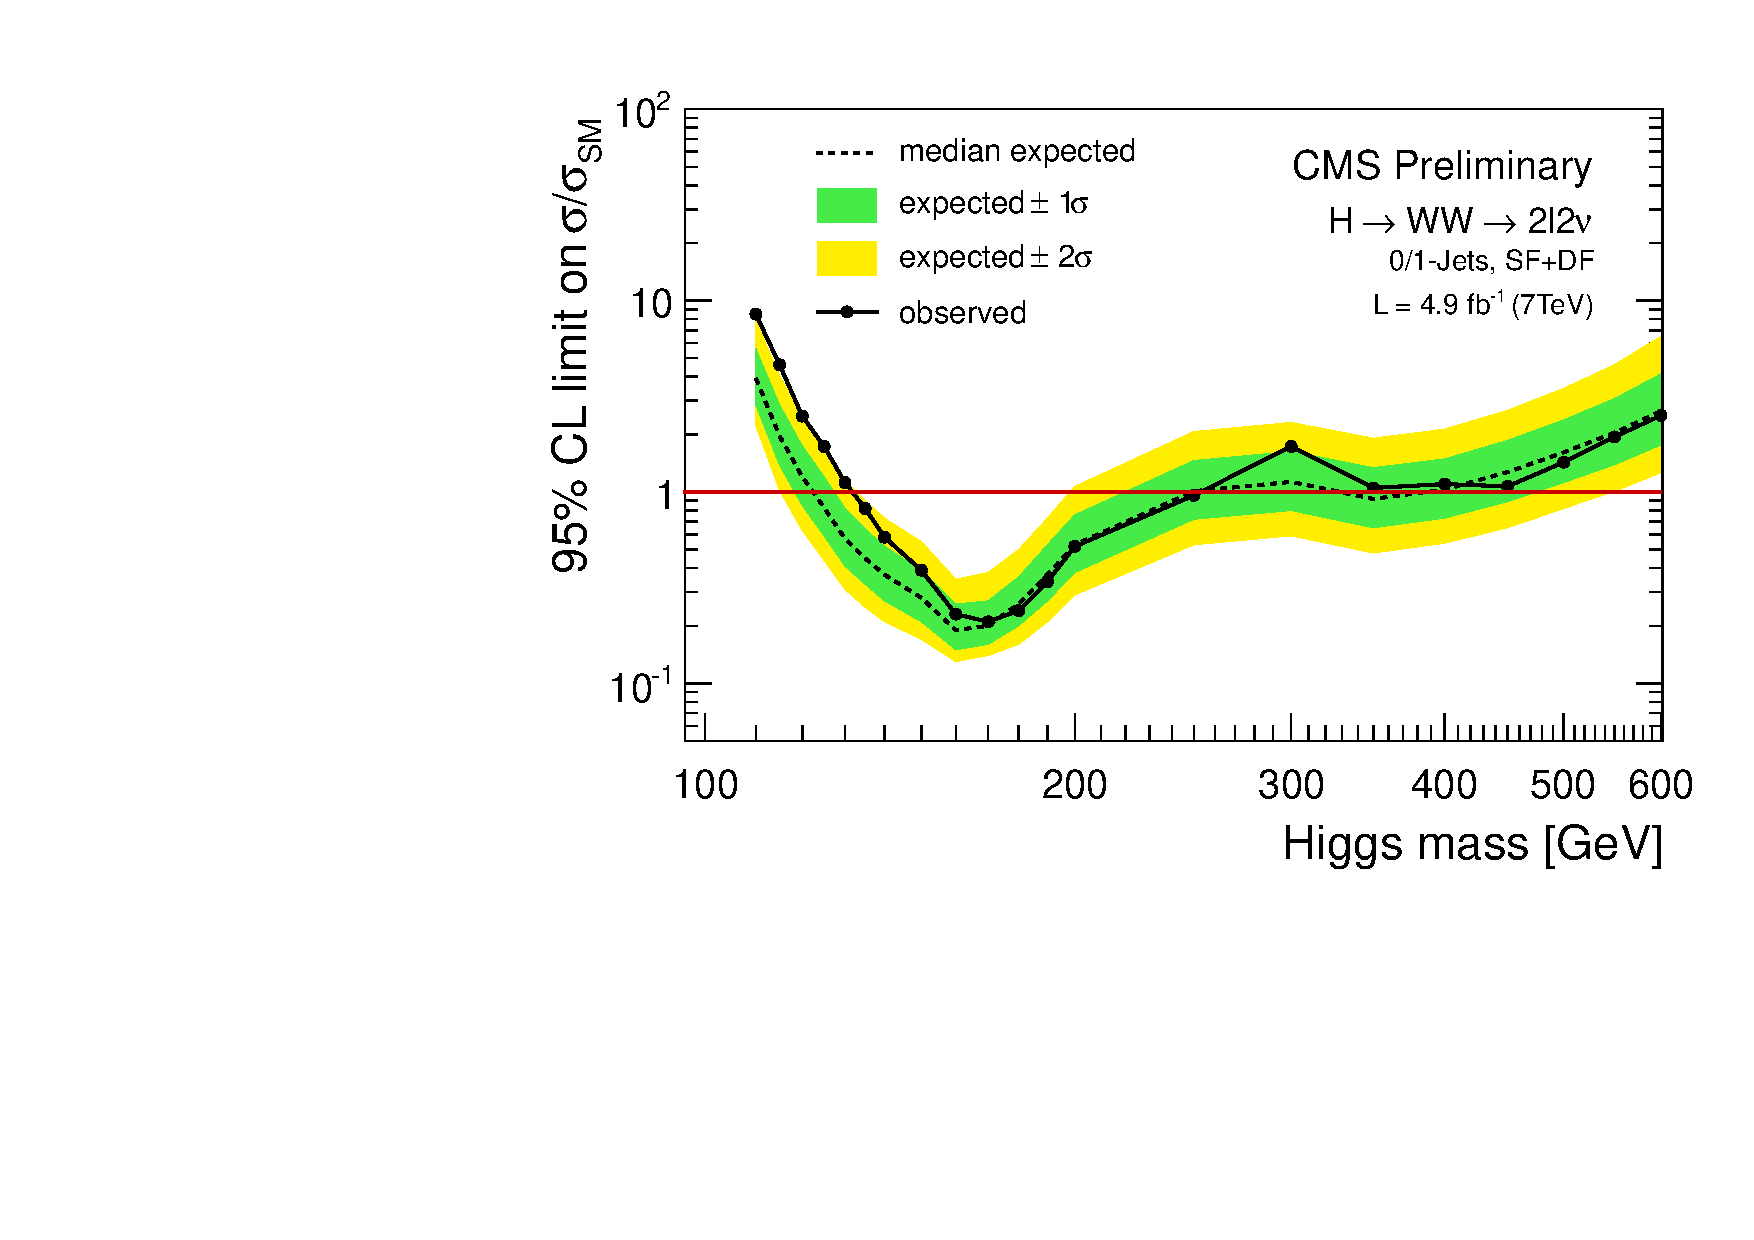
\includegraphics[width=.75\textwidth]{figures/table_limits_nj_7TeV_log.pdf}
\caption{Observed and expected upper limits for SM Higgs in $\intlumiEightTeV$ at 8 TeV in 0/1jet final state. 
2D(cut-based) analysis is used in the DF(SF) final states.}  
\label{fig:uls_7tev}
\end{figure}
% table
\begin{table}[!htbp]
\begin{center}
\begin{tabular}{c c c c c}
\hline
\vspace{-3mm} && \\
Higgs Mass & Observed  & Median expected & Expected range for 68\% & Expected range for 95\%   \\
\hline
110 & 8.50 & 3.93 & [2.85, 5.61] & [2.21, 7.92] \\
115 & 4.62 & 1.96 & [1.38, 2.85] & [1.02, 4.05] \\
120 & 2.49 & 1.20 & [0.85, 1.74] & [0.63, 2.47] \\
125 & 1.73 & 0.83 & [0.59, 1.20] & [0.44, 1.69] \\
130 & 1.12 & 0.57 & [0.41, 0.82] & [0.31, 1.15] \\
135 & 0.82 & 0.45 & [0.33, 0.64] & [0.25, 0.90] \\
140 & 0.58 & 0.37 & [0.27, 0.52] & [0.21, 0.73] \\
150 & 0.39 & 0.28 & [0.21, 0.39] & [0.17, 0.55] \\
160 & 0.23 & 0.19 & [0.15, 0.26] & [0.13, 0.35] \\
170 & 0.21 & 0.20 & [0.16, 0.27] & [0.14, 0.38] \\
180 & 0.24 & 0.26 & [0.20, 0.36] & [0.16, 0.50] \\
190 & 0.34 & 0.37 & [0.27, 0.53] & [0.21, 0.73] \\
200 & 0.52 & 0.53 & [0.38, 0.76] & [0.29, 1.07] \\
250 & 0.96 & 1.01 & [0.72, 1.46] & [0.53, 2.07] \\
300 & 1.73 & 1.13 & [0.80, 1.63] & [0.59, 2.31] \\
350 & 1.05 & 0.92 & [0.65, 1.34] & [0.48, 1.91] \\
400 & 1.10 & 1.03 & [0.73, 1.49] & [0.54, 2.13] \\
450 & 1.07 & 1.27 & [0.89, 1.86] & [0.65, 2.67] \\
500 & 1.43 & 1.61 & [1.12, 2.38] & [0.82, 3.48] \\
550 & 1.94 & 2.04 & [1.39, 3.08] & [1.01, 4.63] \\
600 & 2.51 & 2.64 & [1.76, 4.14] & [1.26, 6.50] \\
\vspace{-3mm} && \\
\hline
\end{tabular}
\caption{Observed and expected upper limits for SM Higgs in $\intlumiEightTeV$ at 8 TeV in 0/1jet final state. 
2D(cut-based) analysis is used in the DF(SF) final states.}  
\label{tab:uls_7tev}
\end{center}
\end{table}
%%%%%%%%%%


%%%%%%%%%%%%%%%%%
% plot
\begin{figure}[!hbtp]
\centering
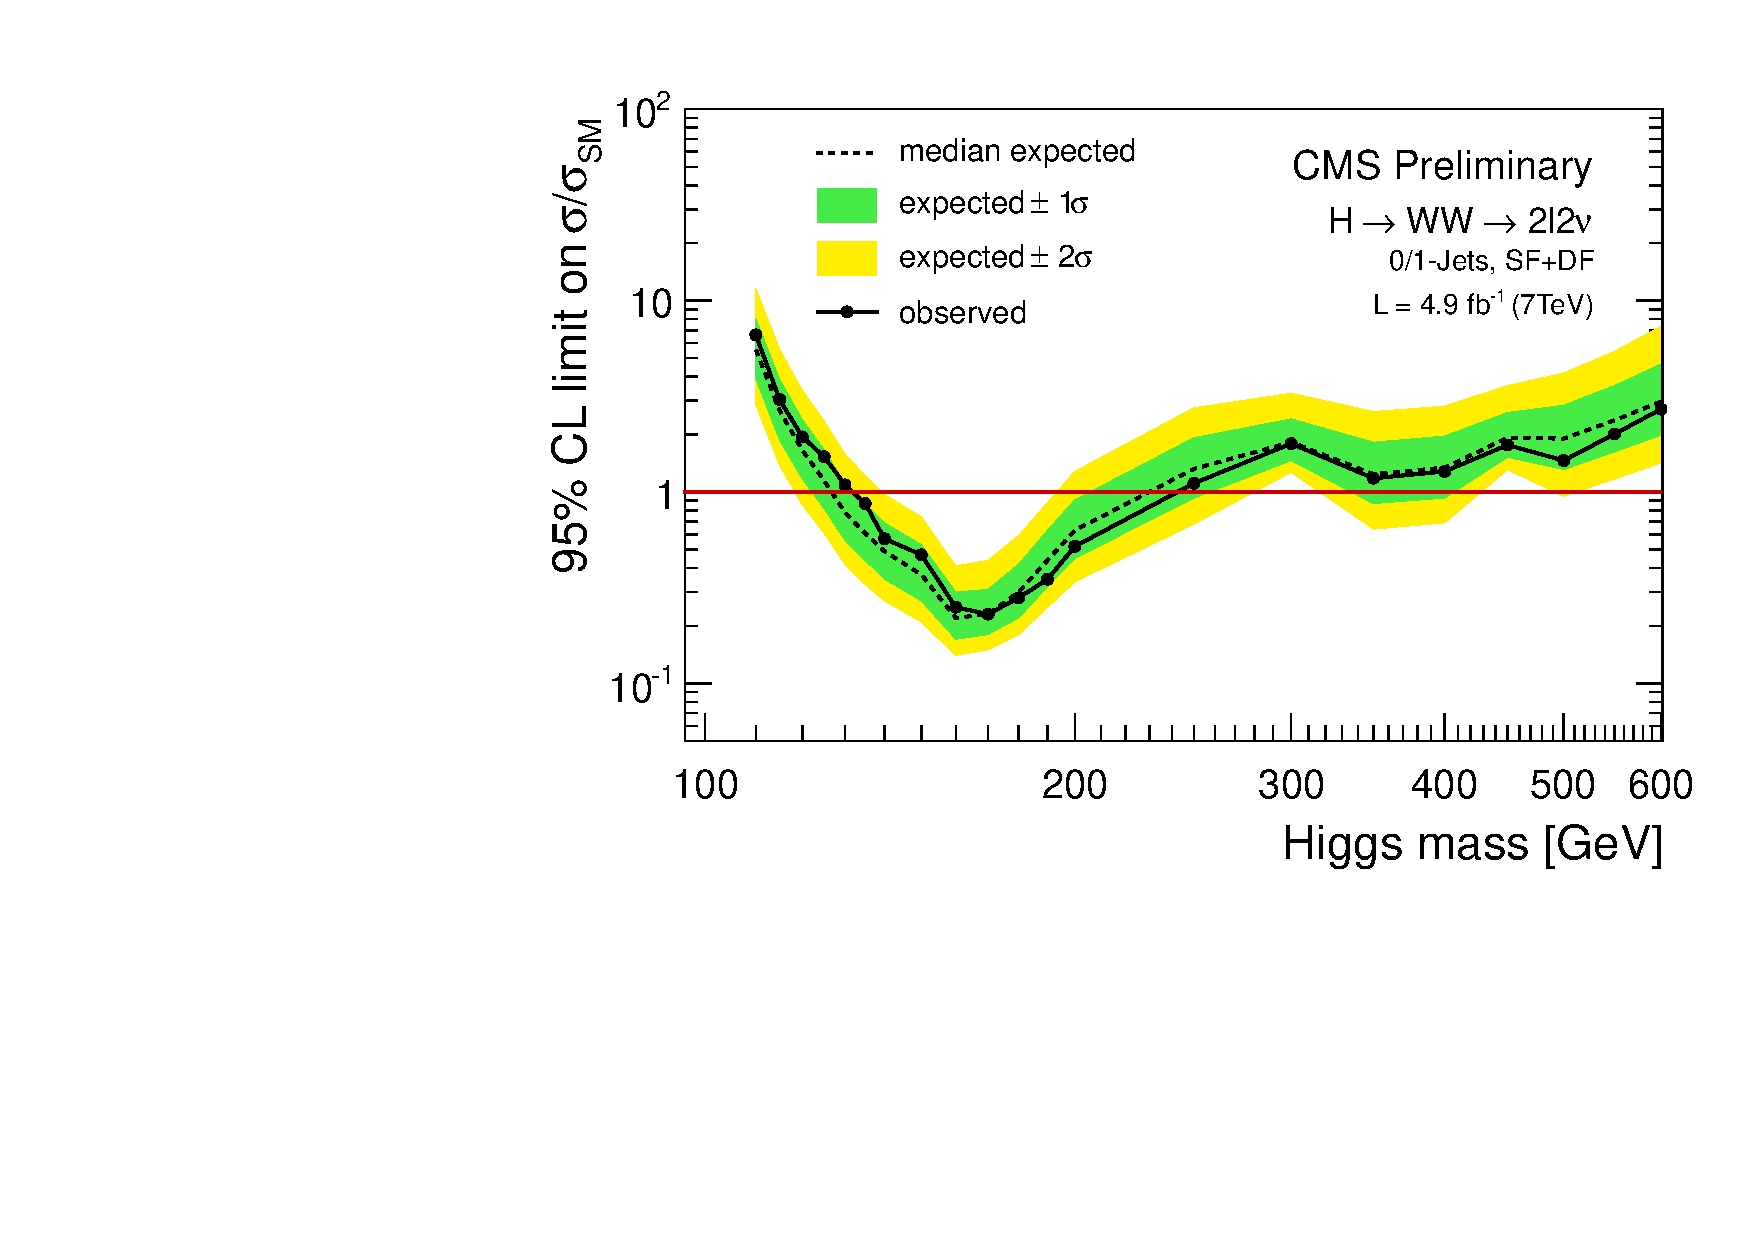
\includegraphics[width=.75\textwidth]{figures/table_limits_nj_cut_7TeV_log.pdf}
\caption{Observed and expected upper limits for SM Higgs in $\intlumiEightTeV$ at 8 TeV in 0/1jet final state. 
Cut-based analysis is used in the DF/SF final states.}  
\label{fig:uls_cut_7tev}
\end{figure}
% table
\begin{table}[!htbp]
\begin{center}
\begin{tabular}{c c c c c}
\hline
\vspace{-3mm} && \\
Higgs Mass & Observed  & Median expected & Expected range for 68\% & Expected range for 95\%   \\
\hline
110 & 6.62 & 5.54 & [3.89, 8.04] & [2.85, 11.53] \\
115 & 3.04 & 2.67 & [1.87, 3.88] & [1.38, 5.56] \\
120 & 1.94 & 1.65 & [1.17, 2.39] & [0.86, 3.39] \\
125 & 1.53 & 1.15 & [0.82, 1.66] & [0.61, 2.35] \\
130 & 1.09 & 0.78 & [0.56, 1.11] & [0.42, 1.57] \\
135 & 0.87 & 0.61 & [0.44, 0.87] & [0.33, 1.22] \\
140 & 0.57 & 0.49 & [0.35, 0.69] & [0.27, 0.97] \\
150 & 0.47 & 0.37 & [0.27, 0.53] & [0.21, 0.74] \\
160 & 0.25 & 0.22 & [0.17, 0.30] & [0.14, 0.41] \\
170 & 0.23 & 0.23 & [0.18, 0.31] & [0.15, 0.44] \\
180 & 0.28 & 0.30 & [0.22, 0.42] & [0.18, 0.59] \\
190 & 0.35 & 0.44 & [0.32, 0.63] & [0.25, 0.88] \\
200 & 0.52 & 0.63 & [0.45, 0.91] & [0.34, 1.28] \\
250 & 1.11 & 1.32 & [0.93, 1.92] & [0.68, 2.75] \\
300 & 1.79 & 1.82 & [1.46, 2.41] & [1.27, 3.28] \\
350 & 1.18 & 1.24 & [0.87, 1.82] & [0.64, 2.63] \\
400 & 1.28 & 1.34 & [0.93, 1.96] & [0.69, 2.81] \\
450 & 1.76 & 1.92 & [1.52, 2.60] & [1.31, 3.59] \\
500 & 1.46 & 1.90 & [1.31, 2.84] & [0.95, 4.18] \\
550 & 2.01 & 2.37 & [1.62, 3.60] & [1.17, 5.43] \\
600 & 2.71 & 2.97 & [1.98, 4.66] & [1.42, 7.33] \\
\vspace{-3mm} && \\
\hline
\end{tabular}
\caption{Observed and expected upper limits for SM Higgs in $\intlumiEightTeV$ at 8 TeV in 0/1jet final state. 
Cut-based analysis is used in the DF/SF final states.}  
\label{tab:uls_cut_7tev}
\end{center}
\end{table}
%%%%%%%%%%

%%%%%%%%
\begin{table}[!htbp]
\begin{center}
\begin{tabular}{c | c c | c c }
\hline \hline 
\vspace{-3mm} && \\ 
                 &  \multicolumn{2}{c}{2D} & \multicolumn{2}{c}{Cut-based} \\
\hline
Higgs Mass(\GeV) & Observed & Expected & Observed & Expected  \\
\hline \hline
110 & 2.56 & 0.56 & 0.48 & 0.38 \\
115 & 2.38 & 1.06 & 0.34 & 0.77 \\
120 & 2.26 & 1.71 & 0.44 & 1.21 \\
125 & 2.26 & 2.45 & 0.79 & 1.72 \\
135 & 1.85 & 4.46 & 0.99 & 3.14 \\
140 & 1.45 & 5.46 & 0.46 & 3.80 \\
150 & 1.17 & 7.20 & 0.76 & 4.96 \\
160 & 0.89 & 10.43 & 0.00 & 8.24 \\
170 & 0.00 & 9.81 & 0.00 & 7.93 \\
180 & 0.00 & 7.20 & 0.00 & 5.86 \\
190 & 0.00 & 5.25 & 0.00 & 3.97 \\
200 & 0.00 & 3.68 & 0.00 & 2.87 \\
250 & 0.00 & 1.96 & 0.00 & 1.51 \\
300 & 1.20 & 1.73 & 0.00 & 1.42 \\
350 & 0.28 & 2.08 & 0.00 & 1.64 \\
400 & 0.20 & 1.87 & 0.00 & 1.53 \\
450 & 0.00 & 1.55 & 0.00 & 1.35 \\
500 & 0.15 & 1.27 & 0.00 & 1.13 \\
550 & 0.93 & 1.06 & 0.00 & 0.94 \\
600 & 0.00 & 0.88 & 0.00 & 0.79 \\
\hline \hline
\end{tabular}
\caption{Observed and expected significances SM Higgs in $\intlumiSevenTeV$ at 7 TeV.  
Cut-based analysis is used in SF final states. Table shows result of all channels combined 
when 2D or cut-based analysis is used in DF 0/1 jet.} 
\label{tab:significance_7tev}
\end{center}
\end{table} 
%%%%%%%%%%%%%%%%%%%%%%%%%%%%%%



%%%%%%%%%%%%%%%%%%%%%%%%%%%%%%
%%%%%%%%%%%%%%%%%%%%%%%%%%%%%%
\clearpage 
\subsection{Final Results for the Higgs Search Combining 7 TeV and 8 TeV Data}
\label{sec:search_results_finalcomb}

The observed and expected upper limits at 95\% C.L. using 2D analysis in DF 0/1 jet categories 
and cut-based analysis in SF 0/1 jet categories are shown in Table~\ref{tab:uls_78tev} and Figure \ref{fig:uls_78tev}.
The observed and expected upper limits at 95\% C.L. using cut-based analysis in DF/SF 0/1 jet categories 
are shown in Table~\ref{tab:uls_cut_78tev} and Figure \ref{fig:uls_cut_78tev}.
The observed and expected significances are shown in Table~\ref{tab:significance_78tev}. 
Figure \ref{fig:uls_78tev_SMH} shows observed and expected upper limits at 95\% C.L.
when SM Higgs at 125 $\GeV$ is considered as a background. The best $\mu$ value as a function 
of the Higgs mass hypothesiswhen SM Higgs at 125 $\GeV$ is considered as a background is shown in 
Figure~\ref{fig:mu_7p8TeV_SMH}. The observed signal strength values for $\mHi = 125~\GeV$ for the different channels used in the shape-based analysis,
together with the combined result, are shown in Figure~\ref{fig:mu_allchannels} and the 
observed signal strength values for all different channels are shown in Table~\ref{tab:mu_allchannels}. 

\begin{table}[!htbp]
\begin{center}
\begin{tabular}{|c | c |}
\hline
  channel &   signal strength \\
\hline
   DF 0-jet bin shape-based 7 $\TeV$ & 0.64 $\pm$ 0.52 \\
   DF 1-jet bin shape-based 7 $\TeV$ & 1.74 $\pm$ 1.01 \\
   DF 0-jet bin shape-based 8 $\TeV$ & 0.69 $\pm$ 0.31 \\
   DF 1-jet bin shape-based 8 $\TeV$ & 0.32 $\pm$ 0.37 \\
     DF 0-jet bin cut-based 7 $\TeV$ & 0.29 $\pm$ 0.68 \\
     DF 1-jet bin cut-based 7 $\TeV$ & 1.00 $\pm$ 1.13 \\
     DF 0-jet bin cut-based 8 $\TeV$ & 0.87 $\pm$ 0.49 \\
     DF 1-jet bin cut-based 8 $\TeV$ & 0.46 $\pm$ 0.50 \\
     SF 0-jet bin cut-based 7 $\TeV$ & 0.16 $\pm$ 1.04 \\
     SF 1-jet bin cut-based 7 $\TeV$ & 0.87 $\pm$ 2.00 \\
     SF 0-jet bin cut-based 8 $\TeV$ & 1.08 $\pm$ 0.75 \\
     SF 1-jet bin cut-based 8 $\TeV$ & 1.51 $\pm$ 0.87 \\
\hline
         combined cut-based 7 $\TeV$ & 0.45 $\pm$ 0.57 \\
         combined cut-based 8 $\TeV$ & 0.81 $\pm$ 0.39 \\
       combined shape-based 7 $\TeV$ & 0.94 $\pm$ 0.44 \\
       combined shape-based 8 $\TeV$ & 0.72 $\pm$ 0.23 \\
\hline
       combined cut-based 7+8 $\TeV$ & 0.76 $\pm$ 0.37 \\
     combined shape-based 7+8 $\TeV$ & 0.77 $\pm$ 0.21 \\
\hline
\end{tabular}
\caption{Observed signal strength values for $\mHi = 125~\GeV$ for the different channels and combinations.} 
\label{tab:mu_allchannels}
\end{center}
\end{table} 

%%%%%%%%%%%%%%%%%  
% plot
\begin{figure}[!hbtp]
\centering
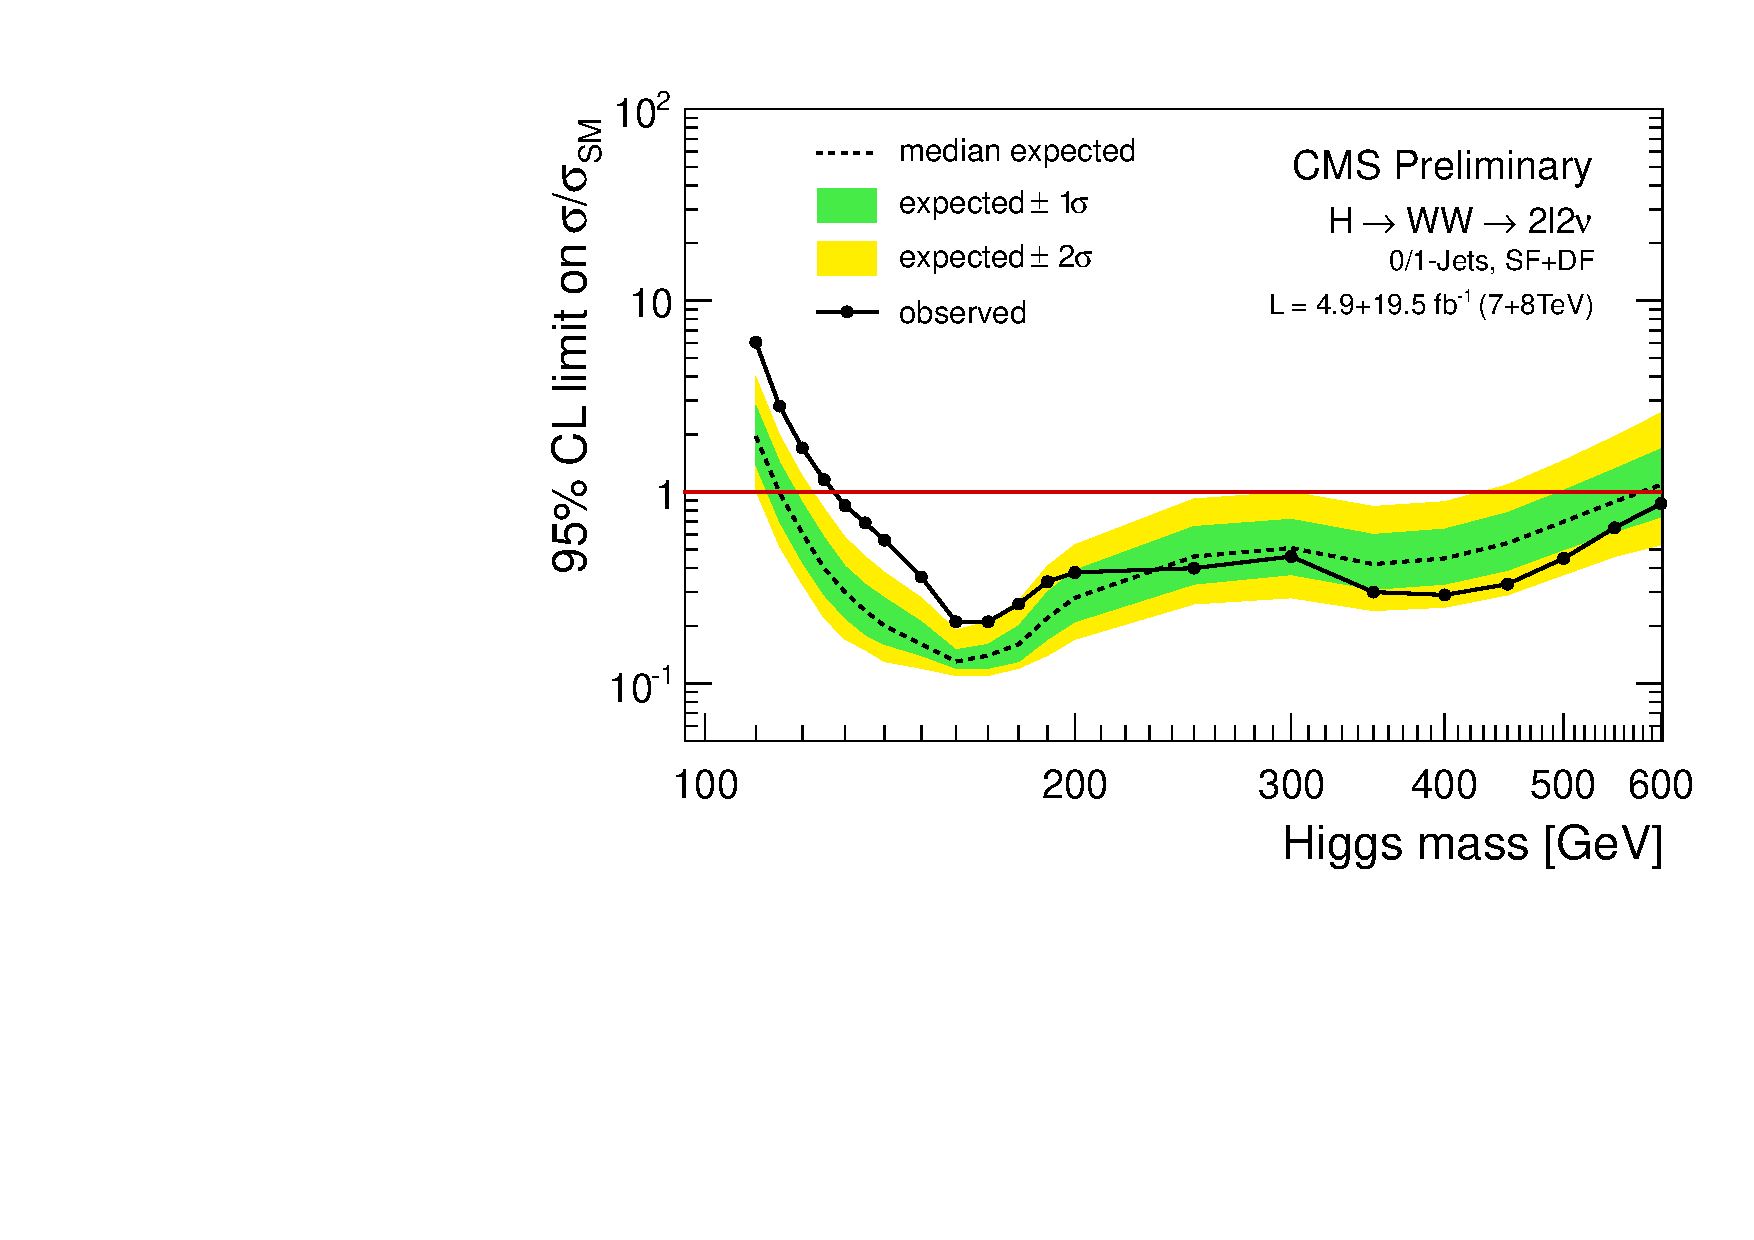
\includegraphics[width=.75\textwidth]{figures/table_limits_nj_78TeV_log.pdf}
\caption{Observed and expected upper limits for SM Higgs in $\intlumiSevenTeV$ at 7 TeV and $\intlumiEightTeV$ at 8 TeV 
in 0/1jet final state. 2D(cut-based) analysis is used in the DF(SF) final states.}  
\label{fig:uls_78tev}
\end{figure}
% table
\begin{table}[!htbp]
\begin{center}
\begin{tabular}{c c c c c}
\hline
\vspace{-3mm} && \\
Higgs Mass & Observed  & Median expected & Expected range for 68\% & Expected range for 95\%   \\
\hline
110 & 6.06 & 1.95 & [1.38, 2.82] & [1.02, 3.99] \\
115 & 2.81 & 0.99 & [0.70, 1.43] & [0.52, 1.98] \\
120 & 1.70 & 0.61 & [0.43, 0.88] & [0.33, 1.21] \\
125 & 1.16 & 0.40 & [0.29, 0.58] & [0.22, 0.82] \\
130 & 0.85 & 0.30 & [0.22, 0.41] & [0.17, 0.58] \\
135 & 0.69 & 0.24 & [0.18, 0.33] & [0.15, 0.46] \\
140 & 0.56 & 0.20 & [0.16, 0.28] & [0.13, 0.38] \\
150 & 0.36 & 0.16 & [0.14, 0.21] & [0.12, 0.28] \\
160 & 0.21 & 0.13 & [0.12, 0.15] & [0.11, 0.19] \\
170 & 0.21 & 0.14 & [0.12, 0.16] & [0.11, 0.21] \\
180 & 0.26 & 0.16 & [0.13, 0.20] & [0.12, 0.27] \\
190 & 0.34 & 0.22 & [0.17, 0.30] & [0.14, 0.41] \\
200 & 0.38 & 0.28 & [0.21, 0.39] & [0.17, 0.53] \\
250 & 0.40 & 0.46 & [0.33, 0.66] & [0.26, 0.92] \\
300 & 0.46 & 0.51 & [0.37, 0.72] & [0.28, 1.00] \\
350 & 0.30 & 0.42 & [0.31, 0.60] & [0.24, 0.84] \\
400 & 0.29 & 0.45 & [0.33, 0.64] & [0.25, 0.89] \\
450 & 0.33 & 0.54 & [0.39, 0.78] & [0.29, 1.09] \\
500 & 0.45 & 0.70 & [0.50, 1.02] & [0.37, 1.46] \\
550 & 0.65 & 0.89 & [0.62, 1.32] & [0.46, 1.95] \\
600 & 0.87 & 1.09 & [0.74, 1.68] & [0.53, 2.59] \\
\vspace{-3mm} && \\
\hline
\end{tabular}
\caption{Observed and expected upper limits for SM Higgs in $\intlumiSevenTeV$ at 7 TeV and $\intlumiEightTeV$ at 8 TeV 
in 0/1jet final state. 2D(cut-based) analysis is used in the DF(SF) final states.}  
\label{tab:uls_78tev}
\end{center}
\end{table}
%%%%%%%%%%



%%%%%%%%%%%%%%%%%  
% plot
\begin{figure}[!hbtp]
\centering
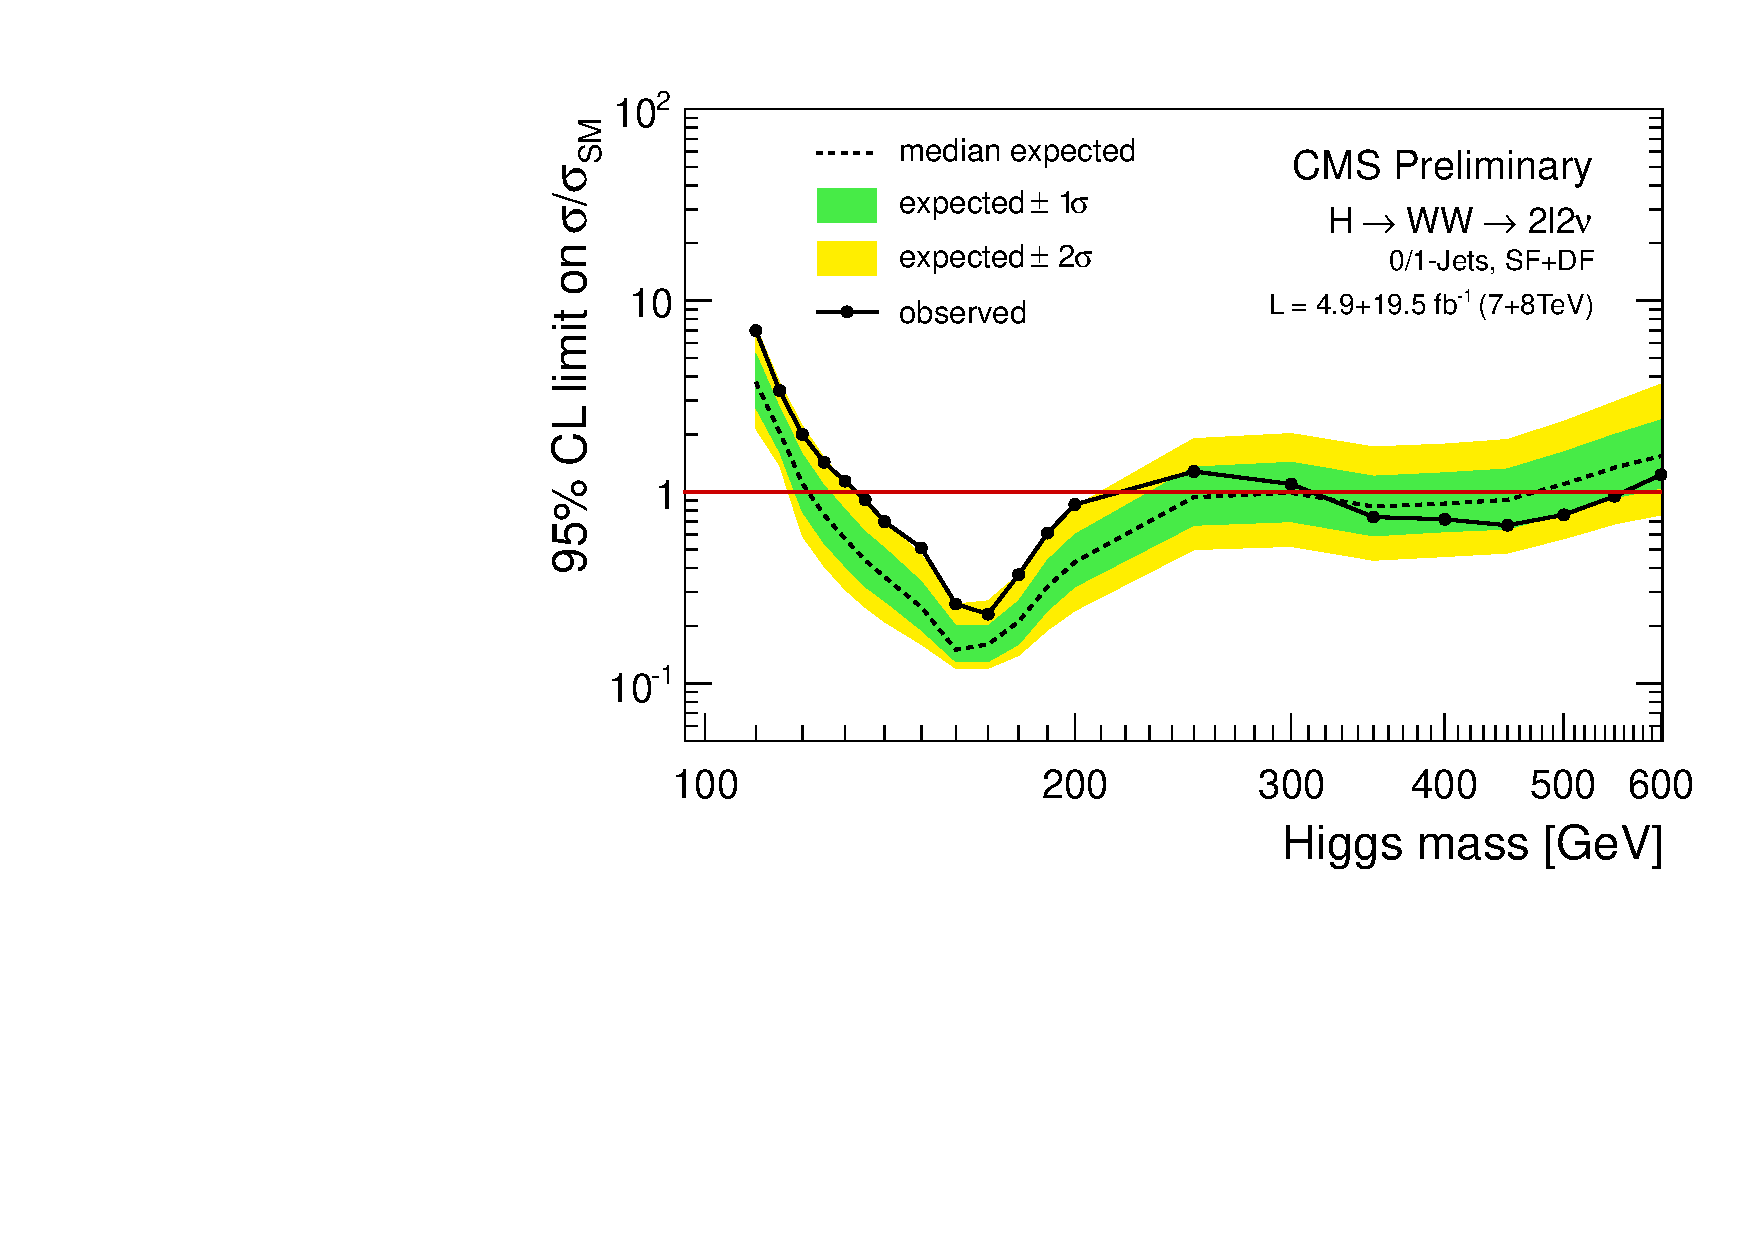
\includegraphics[width=.75\textwidth]{figures/table_limits_nj_cut_78TeV_log.pdf}
\caption{Observed and expected upper limits for SM Higgs in $\intlumiSevenTeV$ at 7 TeV and $\intlumiEightTeV$ at 8 TeV 
in 0/1jet final state. Cut-based analysis is used in the DF/SF final states.}  
\label{fig:uls_cut_78tev}
\end{figure}
% table
\begin{table}[!htbp]
\begin{center}
\begin{tabular}{c c c c c}
\hline
\vspace{-3mm} && \\
Higgs Mass & Observed  & Median expected & Expected range for 68\% & Expected range for 95\%   \\
\hline
110 & 6.97 & 3.75 & [2.75, 5.27] & [2.14, 7.32] \\
115 & 3.39 & 2.06 & [1.62, 2.76] & [1.38, 3.74] \\
120 & 2.00 & 1.11 & [0.79, 1.58] & [0.59, 2.22] \\
125 & 1.43 & 0.76 & [0.54, 1.08] & [0.41, 1.51] \\
130 & 1.14 & 0.57 & [0.41, 0.81] & [0.31, 1.12] \\
135 & 0.91 & 0.44 & [0.32, 0.62] & [0.25, 0.86] \\
140 & 0.70 & 0.36 & [0.27, 0.51] & [0.21, 0.70] \\
150 & 0.51 & 0.25 & [0.19, 0.34] & [0.16, 0.47] \\
160 & 0.26 & 0.15 & [0.13, 0.20] & [0.12, 0.26] \\
170 & 0.23 & 0.16 & [0.13, 0.20] & [0.12, 0.27] \\
180 & 0.37 & 0.21 & [0.16, 0.27] & [0.14, 0.37] \\
190 & 0.61 & 0.32 & [0.24, 0.44] & [0.19, 0.61] \\
200 & 0.86 & 0.43 & [0.32, 0.60] & [0.24, 0.84] \\
250 & 1.28 & 0.94 & [0.67, 1.35] & [0.50, 1.90] \\
300 & 1.10 & 0.99 & [0.70, 1.43] & [0.52, 2.02] \\
350 & 0.74 & 0.84 & [0.59, 1.21] & [0.44, 1.72] \\
400 & 0.72 & 0.87 & [0.62, 1.26] & [0.46, 1.78] \\
450 & 0.67 & 0.91 & [0.64, 1.32] & [0.48, 1.88] \\
500 & 0.76 & 1.10 & [0.77, 1.62] & [0.57, 2.34] \\
550 & 0.95 & 1.34 & [0.93, 2.00] & [0.68, 2.96] \\
600 & 1.23 & 1.54 & [1.05, 2.38] & [0.76, 3.66] \\
\vspace{-3mm} && \\
\hline
\end{tabular}
\caption{Observed and expected upper limits for SM Higgs in $\intlumiSevenTeV$ at 7 TeV and $\intlumiEightTeV$ at 8 TeV 
in 0/1jet final state. Cut-based analysis is used in the DF/SF final states.}  
\label{tab:uls_cut_78tev}
\end{center}
\end{table}
%%%%%%%%%%

%%%%%%%%%%%%%%%%%  
\begin{figure}[!hbtp]
\centering
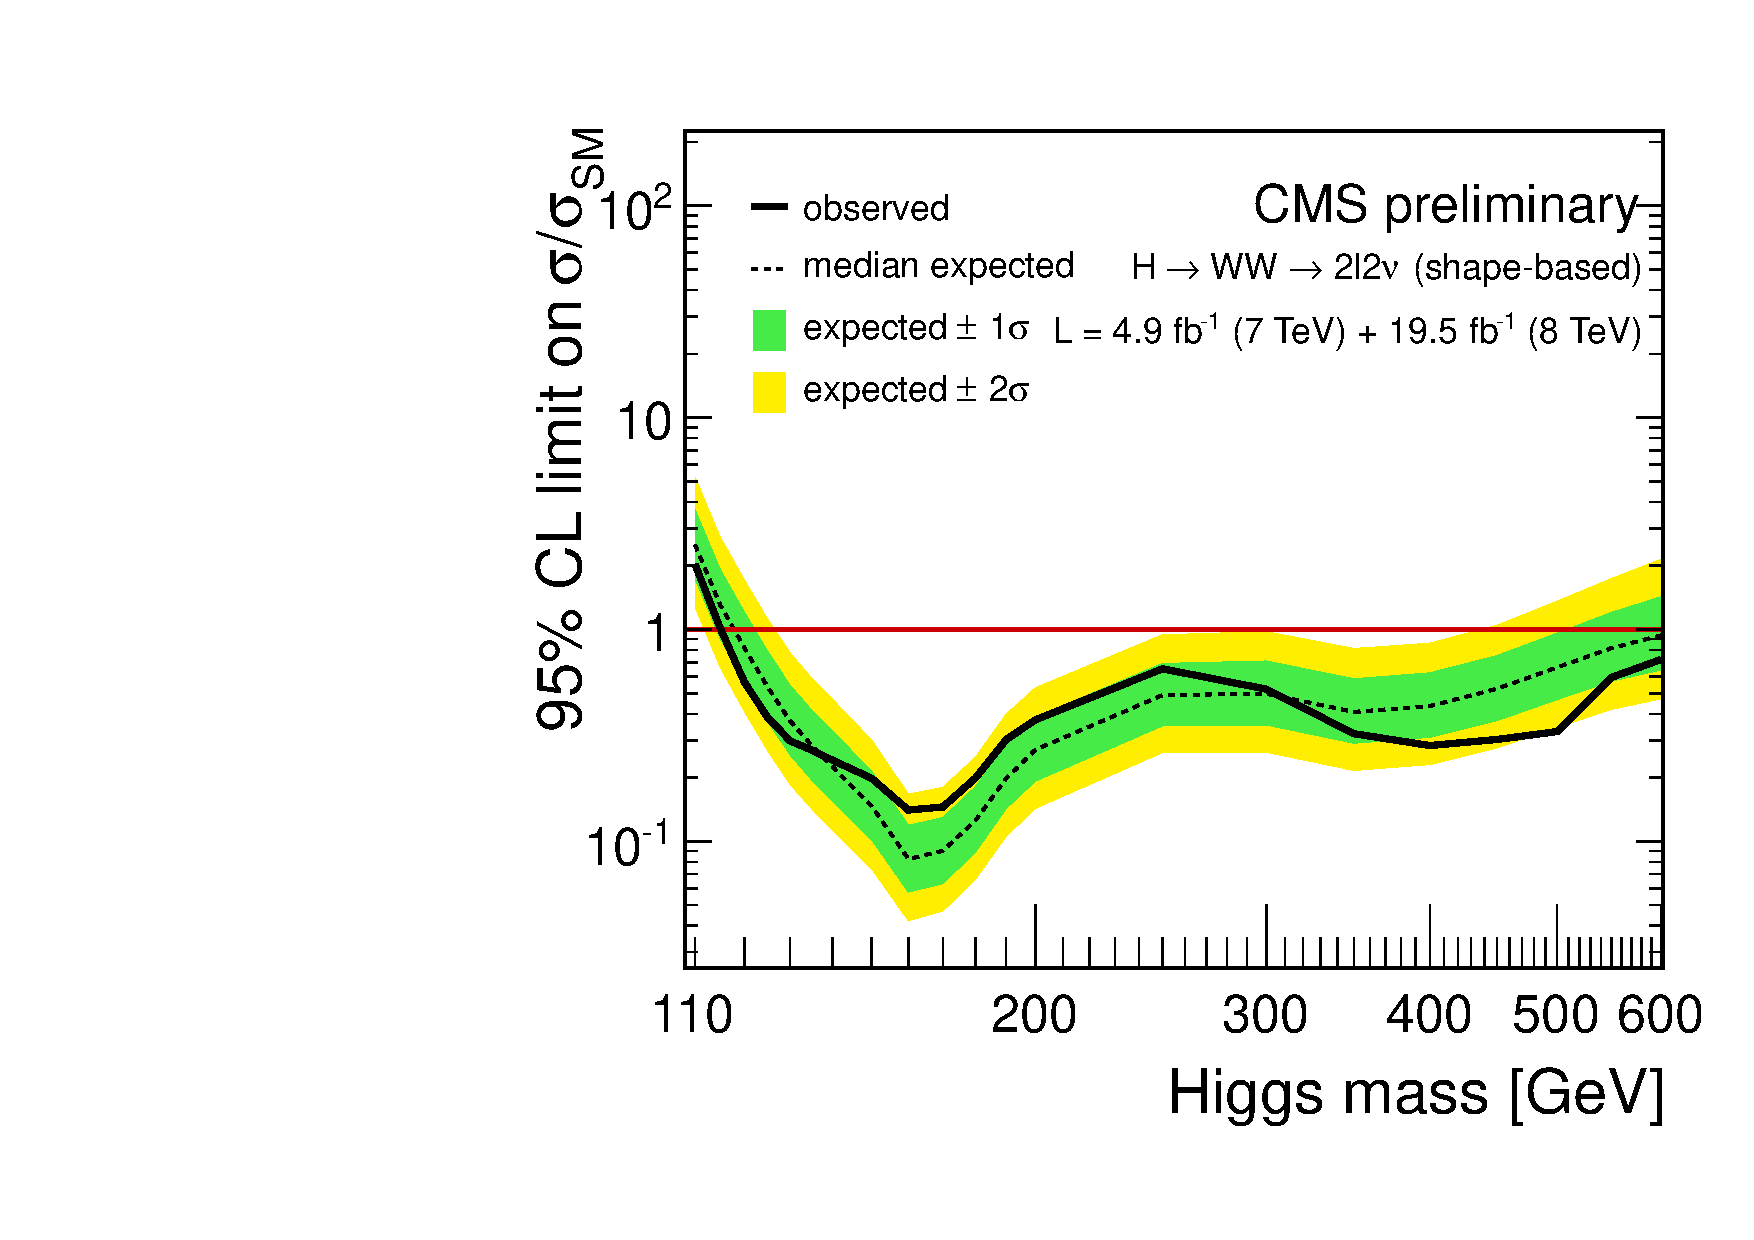
\includegraphics[width=.75\textwidth]{figures/ana_Moriond13_2D_SMH_7p8TeV_bdt_from110to600_logx1_logy1.pdf}
\caption{Observed and expected upper limits considering SM Higgs of \mHi=125\GeV as a background 
in $\intlumiSevenTeV$ at 7 TeV and $\intlumiEightTeV$ at 8 TeV in 0/1jet final state. 
2D analysis is used in the DF/SF final states.}  
\label{fig:uls_78tev_SMH}
\end{figure}

\begin{figure}[!hbtp]
\centering
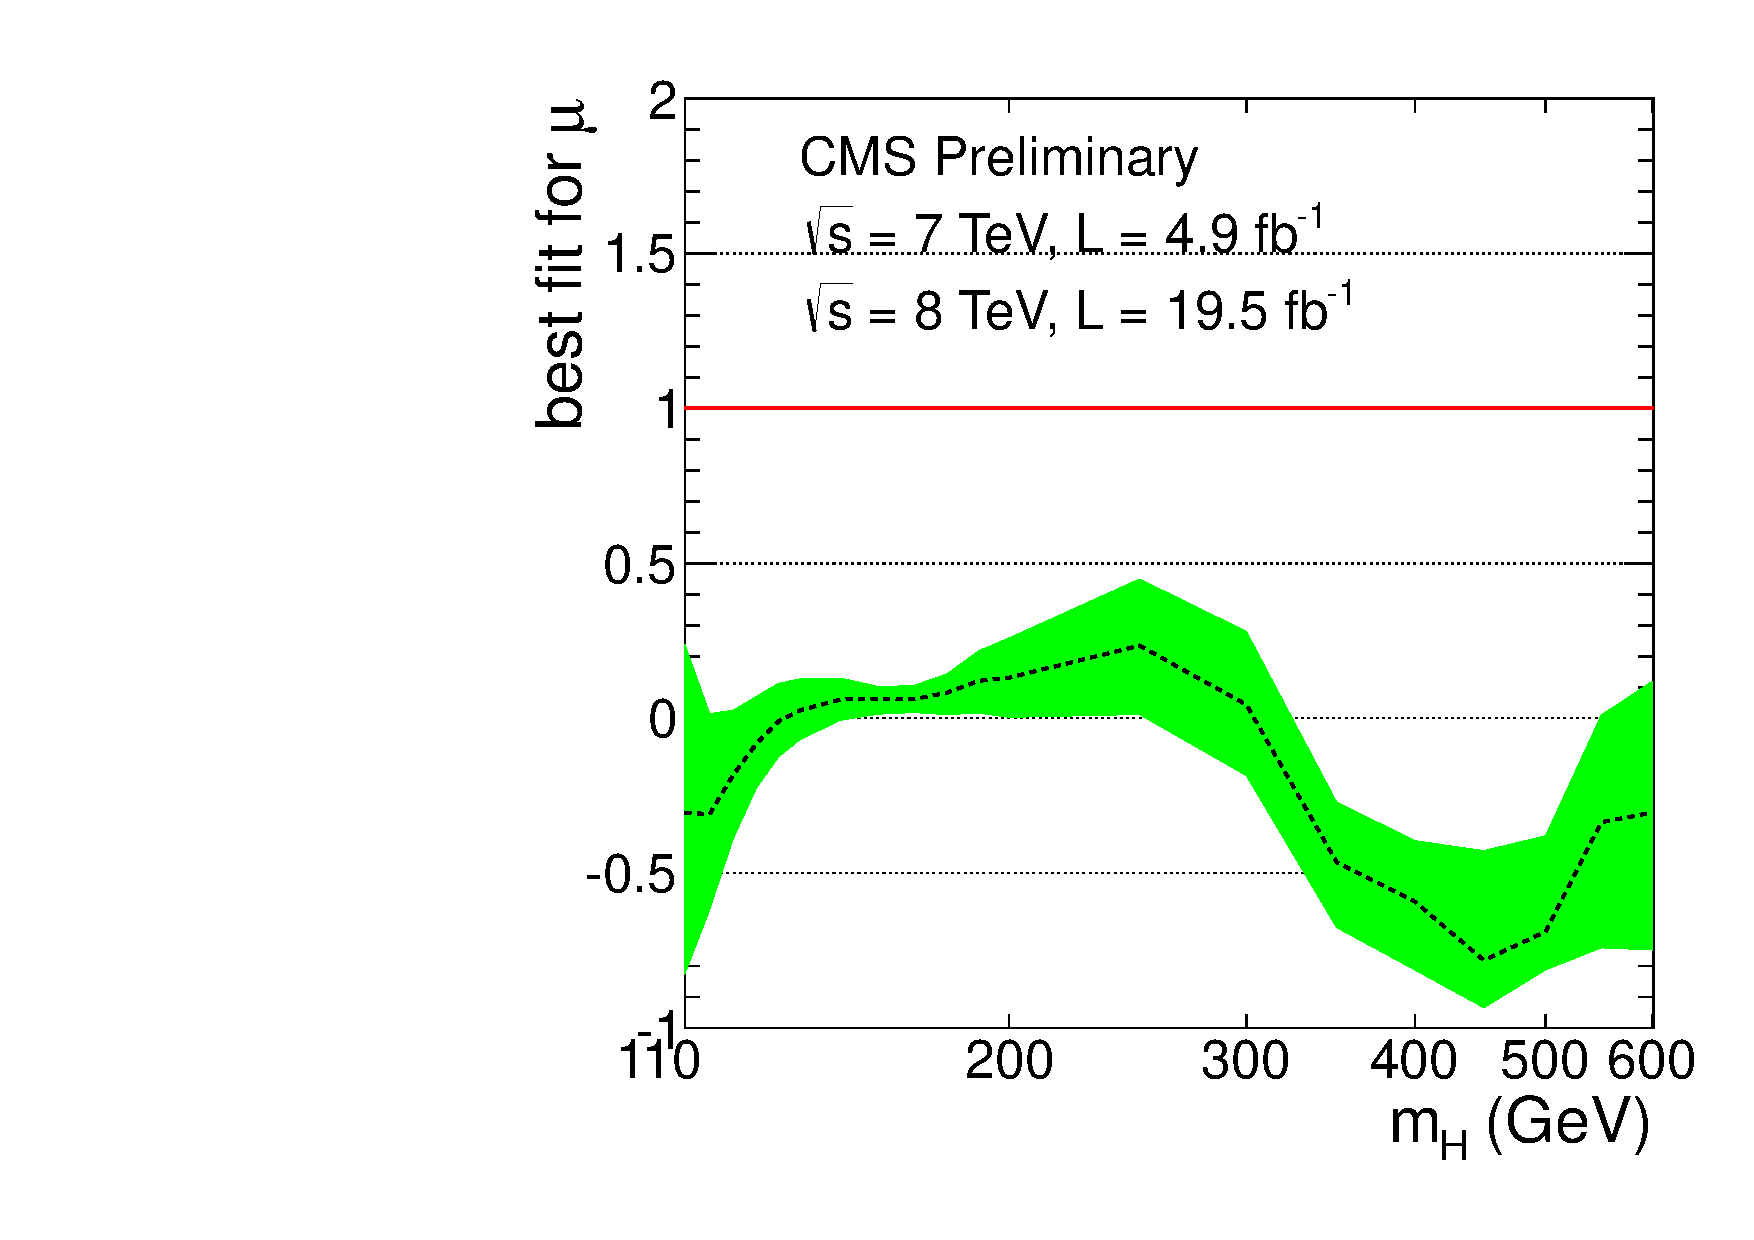
\includegraphics[width=.75\textwidth]{figures/mu_7p8TeV_SMH.pdf}
\caption{Best $\mu$ value considering SM Higgs of $\mHi$ = 125 $\GeV$ as a background.}  
\label{fig:mu_7p8TeV_SMH}
\end{figure}

%%%%%%%%
\begin{table}[!htbp]
\begin{center}
\begin{tabular}{c | c c | c c }
\hline \hline 
\vspace{-3mm} && \\ 
                 &  \multicolumn{2}{c}{2D} & \multicolumn{2}{c}{Cut-based} \\
\hline
Higgs Mass(\GeV) & Observed & Expected & Observed & Expected  \\
\hline \hline
110 & 3.65 & 1.05 & 2.05 & 0.60 \\
115 & 3.83 & 2.04 & 2.05 & 1.19 \\
120 & 3.80 & 3.34 & 1.86 & 1.83 \\
125 & 4.03 & 5.11 & 2.07 & 2.65 \\
130 & 4.25 & 7.15 & 2.34 & 3.46 \\
135 & 4.51 & 9.15 & 2.51 & 4.39 \\
140 & 4.58 & 11.16 & 2.35 & 5.20 \\
150 & 4.18 & 15.16 & 2.78 & 7.46 \\
160 & 4.00 & 22.04 & 2.80 & 11.63 \\
170 & 3.22 & 18.91 & 2.11 & 10.73 \\
180 & 2.65 & 13.12 & 2.36 & 8.42 \\
190 & 2.03 & 9.12 & 2.38 & 5.60 \\
200 & 1.31 & 7.22 & 2.48 & 4.31 \\
250 & 0.00 & 4.18 & 0.91 & 2.05 \\
300 & 0.00 & 3.78 & 0.19 & 1.95 \\
350 & 0.00 & 4.41 & 0.00 & 2.26 \\
400 & 0.00 & 4.10 & 0.00 & 2.16 \\
450 & 0.00 & 3.39 & 0.00 & 2.07 \\
500 & 0.00 & 2.69 & 0.00 & 1.77 \\
550 & 0.00 & 2.18 & 0.00 & 1.52 \\
600 & 0.00 & 1.99 & 0.00 & 1.39 \\
\hline \hline
\end{tabular}
\caption{Observed and expected significances SM Higgs in $\intlumiSevenTeV$ at 7 TeV and $\intlumiEightTeV$ at 8 TeV.  
Cut-based analysis is used in SF final states. Table shows result of all channels combined 
when 2D or cut-based analysis is used in DF 0/1 jet.} 
\label{tab:significance_78tev}
\end{center}
\end{table} 

%%%%%%%%%%%%%%%%%%%%%%%%%%%%%%
\begin{figure}[hbt]
\begin{center}
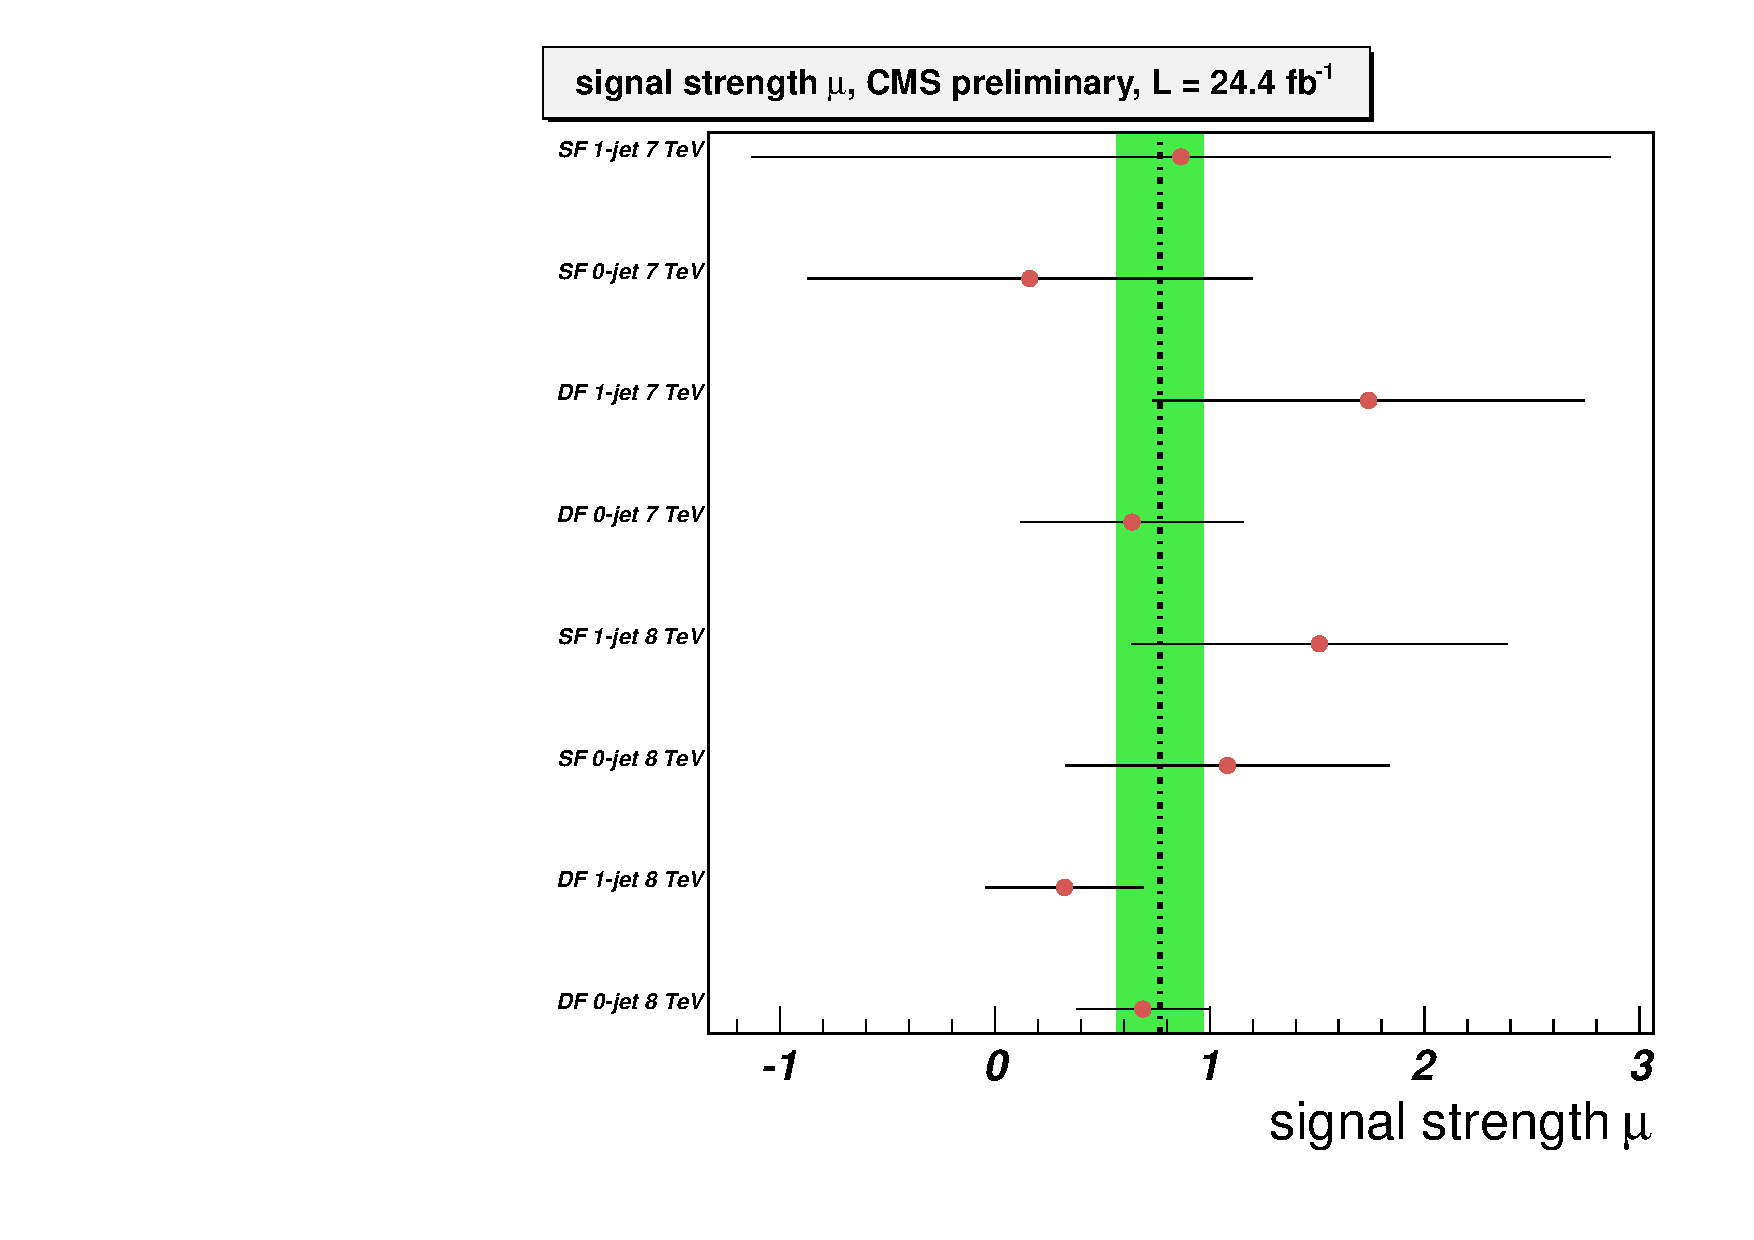
\includegraphics[width=0.85\textwidth]{figures/mu_allchannels.pdf}
\caption{\label{fig:mu_allchannels} Observed signal strength values for 
$\mHi = 125~\GeV$ for the different channels used in the shape-based 
analysis, together with the combined result.}
\end{center}
\end{figure}
%%%%%%%%%%%%%%%%%%%%%%%%%%%%%%
